\documentclass[12pt]{article}
\usepackage{setspace}
\usepackage[utf8]{inputenc}
\usepackage{graphicx}
\usepackage{titling}
\usepackage{tocloft}
\usepackage{titlesec}
\usepackage[letterpaper, left=3cm, right=2cm, top=2cm, bottom=2cm]{geometry}
\usepackage{datetime}
\usepackage{caption}
\usepackage{wrapfig}
\usepackage{microtype}
\usepackage{tabularx}
\usepackage{multirow}
\usepackage{tocloft}
\usepackage{amsmath}
\usepackage{gensymb}
\usepackage[utf8]{inputenc}
\usepackage{array}
\usepackage[table,xcdraw]{xcolor}
\usepackage{subfig}
\usepackage{tikz}
\usepackage{amssymb}
\usepackage[utf8]{inputenc}
\usepackage{colortbl}
\usepackage[table]{xcolor}
\usepackage{geometry}
\geometry{margin=1cm}
\usepackage{longtable}
\captionsetup[figure]{font=small, labelformat=empty}
\renewcommand{\contentsname}{Índice}
\renewcommand{\listfigurename}{Tabla de figuras}
\renewcommand{\tablename}{Tabla}

\usepackage{xurl} % Permite saltos de línea en cualquier parte de una URL
\usepackage[style=apa, backend=biber, natbib=true]{biblatex}
\addbibresource{fonts.bib} 
\setcounter{biburllcpenalty}{100}
\setcounter{biburlucpenalty}{100}
\setcounter{biburlnumpenalty}{100}
\appto{\bibsetup}{\sloppy}

\usepackage{xcolor}       % Para colores
\usepackage{listings}     % Para mostrar código

% Configuración de listings para JSON
\lstdefinestyle{json}{
    basicstyle=\ttfamily\footnotesize,
    commentstyle=\color{gray},
    numbers=left,
    numberstyle=\tiny\color{gray},
    stepnumber=1,
    numbersep=5pt,
    backgroundcolor=\color{white},
    showspaces=false,
    showstringspaces=false,
    showtabs=false,
    frame=single,
    rulecolor=\color{black},
    tabsize=2,
    breaklines=true,
    breakatwhitespace=true,
    stringstyle=\color{blue},
    keywordstyle=\color{red},
    identifierstyle=\color{black},
    literate=
        *{0}{{{\color{red}0}}}{1}
        {1}{{{\color{red}1}}}{1}
        {2}{{{\color{red}2}}}{1}
        {3}{{{\color{red}3}}}{1}
        {4}{{{\color{red}4}}}{1}
        {5}{{{\color{red}5}}}{1}
        {6}{{{\color{red}6}}}{1}
        {7}{{{\color{red}7}}}{1}
        {8}{{{\color{red}8}}}{1}
        {9}{{{\color{red}9}}}{1}
        {:}{{{\color{purple}{:}}}}{1}
        {,}{{{\color{purple}{,}}}}{1}
        {\{}{{{\color{black}{\{}}}}{1}
        {\}}{{{\color{black}{\}}}}}{1}
        {[}{{{\color{black}{[}}}}{1}
        {]}{{{\color{black}{]}}}}{1},
}

% Configuración de la página
\geometry{a4paper, margin=2.5cm}
\setlength{\parindent}{0cm}

% Configuración de los títulos
\titleformat{\section}[block]{\centering\bfseries\Large}{}{0em}{}
\titlespacing*{\section}{0cm}{2cm}{1cm}

\begin{document}
\begin{titlepage}
    \centering
    \includegraphics[width=3cm]{logo umayor.png}
    
    \vspace{2cm}
    
    \textbf{\LARGE Ingeniería Civil en Computación e Informática.}
    
    \vspace{1cm}
    \textbf{\Large Facultad de Ciencias, Ingeniería y Tecnología.}
    \vspace{1cm}
    \textbf{\\Proyecto de Ingeniería II}
    
    \vspace{1cm}
    \section*{\LARGE Solución tecnológica para la gestión, cruce de datos y análisis del entrenamiento concurrente y nutrición en deportistas aficionados.}
    
    \vspace{2cm}
    \begin{flushleft}
    \textbf{}\\
        \begin{tabular}{ll}
    \\
        \end{tabular}
    
    \vspace{0.5cm}
    \textbf{Por:} \\
    Diego Enrique Vilches Jiménez\\
    \vspace{1cm}
    \vspace{2cm}
    \end{flushleft}
    Octubre - 2026
\end{titlepage}
\tableofcontents
\newpage
\listoffigures
\newpage
\setstretch{1.5}
\newpage
\section{Introducción}
\subsection{Contexto General del Área}
El deporte ha evolucionado desde una necesidad básica de supervivencia hacia una práctica altamente especializada. Hoy en día, las metodologías de entrenamiento y optimización de recursos energéticos del ámbito profesional han sido adoptadas masivamente por deportistas aficionados. Esto se refleja en el uso extendido de tecnologías para medir el rendimiento, como smartwatches, bandas cardíacas y ciclocomputadores.
\\\\
En este escenario surge la figura del atleta híbrido: una persona enfocada en desarrollar simultáneamente dos áreas que suelen competir entre sí: la fuerza máxima (como el levantamiento de pesas) y la resistencia cardiovascular (como el ciclismo de ruta o el running). En el ámbito de la medicina, esta práctica se conoce como entrenamiento concurrente, definido como la combinación sistemática de entrenamiento de fuerza y entrenamiento de resistencia dentro de un mismo programa \citep{fisiologiadelejercicio}.
\\\\
Para estos deportistas, mantener una base nutricional sólida y evitar que los entrenamientos interfieran negativamente entre sí resulta crucial. Sin embargo, la gestión inadecuada de estas variables genera altos niveles de fatiga y un progreso nulo o limitado \citep{fisiologiadelejercicio}. Las aplicaciones actuales operan de forma aislada: proponen objetivos de levantamiento de pesas sin considerar si el atleta tiene planificado un fondo largo en bicicleta al día siguiente, o si cumplió con sus requerimientos de macronutrientes. Al no existir un cruce de datos, el usuario no puede medir la fatiga real acumulada ni optimizar su recuperación.
\newpage
\subsection{Motivación del proyecto}
La motivación principal de este proyecto surge de la necesidad de registrar y gestionar de manera efectiva el progreso en el entrenamiento concurrente, específicamente al combinar disciplinas de fuerza con deportes de resistencia como el ciclismo de ruta. Con frecuencia, la falta de cruce de datos provoca que las sesiones de resistencia se realicen con fatiga muscular acumulada de días anteriores, o que el rendimiento en el levantamiento de pesas disminuya tras un esfuerzo cardiovascular prolongado. Controlar estas variables se vuelve aún más crítico cuando el deportista busca mantener un déficit calórico.
\\\\
Actualmente, el uso de aplicaciones nutricionales convencionales permite estimar el gasto energético y contabilizar calorías con eficacia para objetivos aislados, como ganar masa muscular o perder grasa. Sin embargo, estas herramientas resultan insuficientes cuando se requiere cruzar las variables nutricionales con la carga de entrenamiento. Por otro lado, las alternativas de gestión manual, como el registro en papel apoyado por consultas a modelos de inteligencia artificial, ofrecen mayor flexibilidad, pero dependen enteramente de estimaciones subjetivas y sensaciones. Esto impide contar con métricas exactas para comparar el progreso real a lo largo del tiempo.
\\\\
Esta limitación refleja la realidad de múltiples aficionados al entrenamiento concurrente que buscan progresar de forma equitativa en ambas disciplinas. A pesar del sólido fundamento teórico existente sobre el manejo de cargas y fatiga, su aplicación práctica resulta compleja sin la intervención de un entrenador experimentado, lo que evidencia la necesidad de un sistema tecnológico capaz de unificar y analizar estas variables.
\newpage
\subsection{Descripción del Problema}
El problema central radica en la fragmentación y falta de integración de las herramientas tecnológicas disponibles para la gestión del entrenamiento concurrente. En la actualidad, los atletas que combinan disciplinas de fuerza y resistencia se ven obligados a utilizar múltiples aplicaciones de forma simultánea: una plataforma especializada para registrar el levantamiento de pesas, otra para monitorear las actividades cardiovasculares y una tercera para el control nutricional.
\\\\
Si bien existen algunas aplicaciones en el mercado orientadas al atleta híbrido, estas suelen ser deficientes o carecer del nivel de detalle necesario en áreas clave. Por ejemplo, es común encontrar herramientas que monitorean adecuadamente el esfuerzo cardiovascular, pero no permiten un registro preciso de la progresión de cargas en el gimnasio, o bien omiten por completo el seguimiento detallado de macronutrientes. Actualmente, no existe una implementación robusta que integre estas tres áreas ---fuerza, resistencia y nutrición--- de manera sencilla y unificada; no obstante, en la siguiente sección se analizarán con mayor detalle las alternativas existentes y se realizará un desglose de sus deficiencias.
\\\\
La principal consecuencia de contar con ecosistemas separados es que los datos operan de forma aislada. Al no existir un cruce de variables entre la dieta consumida, el volumen de fuerza y la intensidad del esfuerzo cardiovascular, se pierde la capacidad de medir la fatiga real acumulada. Esto imposibilita que los sistemas actuales ofrezcan recomendaciones proactivas sobre cómo ajustar la carga de entrenamiento del día siguiente, modificar la ingesta de alimentos para recuperar glucógeno o gestionar los tiempos de descanso, lo que facilita el sobreentrenamiento y frustra el progreso del usuario.
\\\\
La relevancia de este problema radica en el crecimiento sostenido de deportistas aficionados que buscan imitar metodologías de alto rendimiento. Al no contar con un equipo multidisciplinario de entrenadores, estos atletas dependen enteramente de herramientas tecnológicas para autogestionarse. La brecha tecnológica actual, donde la información de nutrición, fuerza y resistencia existe en silos aislados, representa una barrera significativa para la práctica segura y efectiva del entrenamiento concurrente.
\\\\
El impacto directo de esta fragmentación recae sobre la salud física y el rendimiento del deportista. La incapacidad de cruzar variables impide dimensionar la carga metabólica y neuromuscular real, lo que lleva frecuentemente a escenarios de sobreentrenamiento en los que el usuario acumula niveles críticos de fatiga cruzada sin advertirlo, hasta que experimenta estancamiento, dolor crónico o lesiones físicas.
\\\\
Además, a nivel psicológico y práctico, la fricción que genera intentar sincronizar manualmente múltiples aplicaciones y calcular empíricamente los requerimientos de recuperación produce un alto nivel de desgaste. Esta complejidad operativa es una de las principales causas de frustración y abandono, ya que el atleta percibe que equilibrar ambas disciplinas resulta insostenible a largo plazo sin sacrificar su bienestar general.
\newpage
\subsection{Revisión Preliminar de Soluciones Existentes}
Existen numerosas aplicaciones relacionadas con el mundo del deporte y la nutrición; entre ellas se destacan:
\begin{itemize}
    \item \textbf{Fitia:} Es una de las aplicaciones más reconocidas en el ámbito de la planificación nutricional. Su funcionalidad principal radica en la estimación del gasto energético y la distribución de macronutrientes, generando planes de alimentación automatizados para objetivos de recomposición corporal (pérdida de grasa o ganancia muscular).
    \\\\
    Sin embargo, frente a la problemática del entrenamiento concurrente, Fitia presenta limitaciones significativas. Su alcance se restringe casi exclusivamente al área dietética. Aunque permite registrar calorías quemadas durante el ejercicio, carece de herramientas para documentar la progresión de cargas en el entrenamiento de fuerza o el impacto fisiológico de las sesiones de resistencia cardiovascular. Al no integrar estas métricas, la aplicación no puede evaluar el desgaste físico real ni la fatiga cruzada, limitándose a ser una herramienta aislada que no optimiza la recuperación deportiva integral del usuario.

    \item \textbf{Threshold y Edge:} Son aplicaciones de reciente desarrollo diseñadas específicamente para el atleta híbrido. Su principal fortaleza es la gestión del entrenamiento concurrente, adaptando las rutinas diariamente; por ejemplo, alejando los días de sentadillas pesadas de los días de carrera larga para evitar la fatiga cruzada.
    \\\\
    A pesar de su eficacia en el ámbito físico, su solución es parcial. Al carecer de un módulo nutricional integrado, no ajustan de forma dinámica la ingesta calórica ni los macronutrientes con base en el desgaste real de las sesiones. Esto deja la recuperación nutricional a la estimación manual del usuario.
\newpage
    \item \textbf{Kenso:} Representa una alternativa analítica que utiliza inteligencia artificial para identificar patrones de estancamiento. Permite registrar rutinas de fuerza e importar datos cardiovasculares desde dispositivos externos (como Garmin o Apple Health), cruzando esta información para alertar sobre sobreentrenamiento.
    \\\\
    Su limitación radica en que sigue obligando al usuario a depender de ecosistemas de terceros para capturar la telemetría del esfuerzo cardiovascular. Además, al igual que las opciones anteriores, no resuelve la integración del seguimiento nutricional dentro del mismo ecosistema.

    \item \textbf{Hybrid:} Es la plataforma actual que más se acerca a una solución unificada. Calcula objetivos diarios de calorías y macronutrientes basándose en el calendario de entrenamiento, priorizando distintos sustratos energéticos según la disciplina del día.
    \\\\
    Aunque aborda la problemática de forma más completa, carece de herramientas orientadas a reducir la fricción diaria del usuario, como la telemetría directa (GPS nativo) o el escalado automático de porciones mediante un módulo social de recetas, características fundamentales para asegurar la adherencia a largo plazo.
\end{itemize}
\newpage
A modo de resumen, la siguiente tabla expone cómo las alternativas actuales abordan los distintos aspectos de la problemática en comparación con la solución integral propuesta en este proyecto:

\vspace{0.5cm}

% Tabla comparativa de soluciones
\begin{table}[h!]
    \centering
    \renewcommand{\arraystretch}{1.5}
    \begin{tabular}{|m{5cm}|c|c|c|c|}
        \hline
        \rowcolor[HTML]{EFEFEF}
        \textbf{Aspecto a resolver} & \textbf{Fitia} & \textbf{Threshold} & \textbf{Kenso} & \textbf{Hybrid} \\ \hline
        Registro de fuerza y cargas & $\times$ & \checkmark & \checkmark & \checkmark \\ \hline
        Seguimiento cardiovascular & $\times$ & \checkmark & Parcial & \checkmark \\ \hline
        Seguimiento nutricional & \checkmark & $\times$ & $\times$ & \checkmark \\ \hline
        Gestión de fatiga cruzada & $\times$ & \checkmark & \checkmark & \checkmark \\ \hline
        Nutrición dinámica por sesión & $\times$ & $\times$ & $\times$ & \checkmark \\ \hline
        Telemetría GPS integrada & $\times$ & $\times$ & $\times$ & $\times$ \\ \hline
        Comunidad y recetas adaptables & $\times$ & $\times$ & $\times$ & $\times$ \\ \hline
        \rowcolor[HTML]{EFEFEF}
        \textbf{Ecosistema 100\% unificado} & $\times$ & $\times$ & $\times$ & Parcial \\ \hline
    \end{tabular}
    \caption{Comparativa de soluciones existentes frente a la propuesta.}
\end{table}
\newpage
\subsection{Comentarios Generales del Capítulo}
En este capítulo se definió al atleta híbrido ---o practicante de entrenamiento concurrente--- como aquella persona cuyo objetivo es progresar tanto en el desarrollo de fuerza máxima como en la resistencia cardiovascular. Dentro de este marco, este tipo de deportistas debe gestionar una gran cantidad de variables. A diferencia de quien solo entrena fuerza, que puede notar entre sesiones cómo se ve afectado su progreso de una manera relativamente sencilla y sabrá que, al consumir una cantidad adecuada de proteínas, podrá progresar sin mayores complicaciones; o de quien se dedica exclusivamente al entrenamiento cardiovascular, que incluirá una mayor proporción de carbohidratos en su dieta para disponer de energía suficiente al momento de entrenar. En general, estos dos mundos por separado pueden llevarse de forma relativamente simple para alguien principiante o con pocos conocimientos teóricos; la complicación comienza cuando se combinan ambos.
\newpage
\section{Planteamiento del Problema}
\subsection{Introducción del Capítulo}
Tal como se expuso en el capítulo anterior, la figura del atleta híbrido presenta necesidades específicas para poder monitorear y evaluar de manera objetiva su progreso real. Dado que el entrenamiento concurrente involucra una compleja interacción de múltiples variables metabólicas y de rendimiento, el registro y control de estos factores resulta prácticamente inviable para una persona sin el apoyo de herramientas tecnológicas externas.
\\\\
Asimismo, se evidenció que, si bien el mercado actual ofrece diversas alternativas para llevar un registro deportivo y nutricional, el problema fundamental radica en su alta fragmentación. El deportista se ve obligado a depender de aplicaciones aisladas que operan en ecosistemas separados y cerrados, lo que confirma la inexistencia actual de una plataforma que ofrezca un entorno unificado capaz de cruzar y analizar todos los datos relevantes de forma integral.
\\\\
En consecuencia, el presente capítulo tiene como propósito profundizar en la problemática metodológica y tecnológica que enfrentan estos deportistas. A lo largo de las siguientes secciones se detallarán las limitaciones operativas derivadas de la falta de integración de datos, cómo esta deficiencia impide medir la fatiga cruzada y de qué manera la fricción provocada por el uso de múltiples herramientas impacta negativamente en el rendimiento, la salud y la motivación del usuario.
\newpage
\subsection{Descripción del Problema}

El problema central que aborda este proyecto es la \textbf{ausencia de un ecosistema tecnológico integrado y unificado para la gestión del entrenamiento concurrente}. En la actualidad, los atletas híbridos carecen de una plataforma capaz de centralizar, cruzar y analizar simultáneamente los datos provenientes del entrenamiento de fuerza, la resistencia cardiovascular y la planificación nutricional de manera automatizada. \\ Para comprender a fondo la naturaleza de esta problemática, resulta fundamental identificar las causas subyacentes que originan esta brecha tecnológica:

\begin{itemize} \item \textbf{Desarrollo de software en silos:} Las aplicaciones deportivas y nutricionales existentes en el mercado están diseñadas para nichos específicos. Existen plataformas robustas exclusivas para la telemetría cardiovascular (como Strava o Garmin Connect), otras para el registro del levantamiento de pesas y otras para el conteo calórico, pero carecen de la interoperabilidad necesaria para comunicarse entre sí.


\item \textbf{Complejidad algorítmica de la fatiga cruzada:} Existe una dificultad técnica inherente al intentar estandarizar en una sola métrica el desgaste neuromuscular (propio de la fuerza) y el estrés metabólico (propio de la resistencia). Al tratarse de sistemas de asimilación de energía distintos, su cuantificación conjunta supone un reto de software que las soluciones actuales no han logrado resolver.
  
  \item \textbf{Modelos nutricionales estáticos:} Las aplicaciones tradicionales de dieta calculan requerimientos fijos y no ajustan de forma dinámica la distribución de macronutrientes en función del desgaste fisiológico diario. Carecen de la capacidad lógica para distinguir si el deportista requiere una reposición agresiva de carbohidratos tras un fondo largo en bicicleta o priorizar proteínas tras una sesión de fuerza máxima.
  
  \item \textbf{Dependencia de la estimación manual:} Ante la falta de automatización y de bases de datos centralizadas, el usuario se ve forzado a actuar como el puente integrador entre sus distintas aplicaciones. Esto le obliga a depender de aproximaciones matemáticas manuales y sensaciones subjetivas para calcular su progreso y programar sus tiempos de recuperación.
\end{itemize}
\newpage
Como consecuencia directa de las causas mencionadas, los deportistas que practican el entrenamiento concurrente sin asistencia profesional directa experimentan una serie de efectos adversos que impactan en su rendimiento, bienestar y adherencia al programa:

\begin{itemize} \item \textbf{Riesgo crítico de sobreentrenamiento y lesiones:} Al no contar con un cruce de variables automatizado, el atleta acumula "fatiga cruzada" de manera silenciosa. La incapacidad de dimensionar la carga real conduce a trabajar sobre tejidos musculares no recuperados, incrementando drásticamente el riesgo de lesiones musculoesqueléticas.


\item \textbf{Estancamiento del rendimiento (Efecto de interferencia):} La mala gestión empírica de las sesiones provoca que entrenamientos de resistencia se realicen con fatiga muscular previa, o que la fuerza máxima se vea mermada tras ejercicios cardiovasculares prolongados. Esta interferencia a nivel fisiológico detiene el progreso equitativo en ambas disciplinas.
  
  \item \textbf{Déficit en la recuperación nutricional:} Al basarse en estimaciones aisladas, los usuarios suelen mantener ingestas que no logran suplir el gasto calórico total ni reparar el daño estructural generado por la concurrencia deportiva. Esto retrasa la adaptación fisiológica y perpetúa el estado de fatiga.
  
  \item \textbf{Alta fricción operativa y desgaste psicológico:} La necesidad constante de sincronizar datos manualmente, cuadrar números metabólicos y reajustar rutinas en múltiples ecosistemas inconexos genera un alto nivel de frustración. Este desgaste operativo es una de las principales causas por las cuales los atletas perciben el estilo de vida híbrido como insostenible y terminan abandonando su planificación a largo plazo.
\end{itemize}

En síntesis, esta relación de causas y efectos evidencia que el problema no reside en la falta de literatura deportiva teórica, sino en la marcada deficiencia de las herramientas tecnológicas actuales para procesar dicha información de manera centralizada y aplicable a la vida diaria del usuario.
\newpage
\subsubsection{Pregunta de Investigación}
En base a la problemática identificada en la sección anterior nos planteamos la siguiente pregunta de investigación:
\begin{center} \Large \textit{¿Cómo sería una propuesta tecnológica unificada para automatizar la gestión y el cruce de datos (fuerza, resistencia y nutrición) del entrenamiento concurrente de los deportistas aficionados en Chile durante el año 2026?} \end{center} \vspace{0.5cm}
\newpage
\subsection{Diagnóstico o contexto actual}
En la actualidad, la programación del entrenamiento deportivo y la preparación física a menudo exigen el desarrollo simultáneo de múltiples capacidades, como la fuerza muscular y la resistencia cardiovascular, una práctica conocida como entrenamiento concurrente. Tradicionalmente, la planificación de estos programas se ha visto obstaculizada por la preocupación en torno al denominado ``efecto de interferencia''. Este concepto sugiere que la combinación simultánea de entrenamiento de fuerza y resistencia aeróbica puede atenuar o inhibir mutuamente las adaptaciones fisiológicas, impactando negativamente sobre todo en el desarrollo de la fuerza, la potencia y la hipertrofia muscular.

Desde una perspectiva molecular, este fenómeno se explica porque el entrenamiento cardiovascular intenso activa rutas metabólicas como la AMPK, la cual puede llegar a inhibir la vía mTOR, principal encargada de la síntesis de proteínas y el crecimiento muscular \citep{aptavs2025concurrente}. Sin embargo, el análisis del entorno científico reciente ha transformado esta perspectiva limitante. La evidencia actual demuestra que el efecto de interferencia no es una barrera absoluta y que el entrenamiento concurrente es, de hecho, compatible con mejoras sustanciales tanto en la capacidad aeróbica como en la hipertrofia muscular para la gran mayoría de la población \citep{fisiologiadelejercicio}. El desafío central hoy en día no reside en una incompatibilidad inherente entre ambas modalidades, sino en la correcta gestión de la dosis de entrenamiento y los periodos de recuperación. 

Estudios exhaustivos han precisado que, cuando el efecto de interferencia se manifiesta, este impacta de manera mucho más pronunciada en las adaptaciones de potencia explosiva que en la fuerza máxima o el crecimiento muscular \citep{fisiologiadelejercicio}. Asimismo, los análisis del entorno advierten que el riesgo de interferencia aumenta considerablemente al realizar sesiones de resistencia prolongadas (superiores a 45-60 minutos) en los mismos días que el trabajo de fuerza \citep{aptavs2025concurrente}. 

Por consiguiente, la situación actual del problema se orienta hacia la optimización de las variables de programación. Para maximizar las adaptaciones y mitigar cualquier posible interferencia, las directrices actuales recomiendan estrategias específicas, como establecer una separación temporal de al menos 6 a 8 horas entre las sesiones \citep{aptavs2025concurrente, fisiologiadelejercicio} o, cuando, por motivos de tiempo, deban realizarse en la misma ventana, priorizar el entrenamiento de fuerza antes que el de resistencia cardiovascular \citep{aptavs2025concurrente}.
\newpage
\subsection{Justificación del Proyecto}

El desarrollo de este proyecto se fundamenta en los múltiples beneficios esperados y su impacto tanto a nivel deportivo como social, destacando dos pilares principales:
\\\\
\textbf{Accesibilidad y democratización del entrenamiento:}\\
Históricamente, el acceso a una gestión avanzada de datos deportivos y entrenamiento personalizado ha estado reservado, en gran medida, para atletas de élite. Sin embargo, este proyecto busca promover la accesibilidad a estas herramientas, permitiendo que más atletas aficionados o en vías de ser profesionales puedan llevar un mejor registro y gestión de sus datos de entrenamiento concurrente desde sus inicios. Al facilitar el acceso a información detallada y estructurada, los deportistas pueden optimizar su progreso sin depender económicamente, desde un principio, de un entrenador. Según la evidencia prospectiva, los avances tecnológicos en el deporte democratizarán el entrenamiento de alta calidad, proporcionando oportunidades de gran valor para atletas amateur que no pueden costear entrenadores presenciales, además de apoyar en la toma de decisiones basada en datos que mejoren el rendimiento deportivo de forma autónoma \citep{frevel2022impact}.
\\\\
\textbf{Recuperación y prevención de lesiones:}\\
Un segundo pilar fundamental del proyecto es minimizar los riesgos de lesiones provocadas por un mal manejo del entrenamiento concurrente (fuerza y resistencia), así como optimizar los procesos de adaptación y recuperación. El análisis automatizado y el cruce de datos posibilitarán alertar sobre posibles riesgos biomecánicos o de sobreentrenamiento, facilitando en su caso la implementación de estrategias o tratamientos fisioterapéuticos que acorten los tiempos de recuperación, permitiendo a los atletas volver a competir en el menor tiempo posible. Al respecto, la tecnificación de los instrumentos de valoración se ha consolidado como un recurso primordial en la gestión deportiva contemporánea. Distintos sistemas tecnológicos se aplican en la actualidad de forma exitosa en los ámbitos de la fisioterapia, acondicionamiento físico y rehabilitación. Diversos expertos de la industria deportiva coinciden en que la recolección y el procesamiento automatizado de datos serán claves en la próxima década para prolongar las carreras deportivas, prevenir lesiones y lograr ventajas competitivas significativas, reduciendo la extrema dependencia del monitoreo humano constante \citep{frevel2022impact}.

\subsection{Objetivos del Proyecto}
\subsubsection{Objetivo General}
Proponer una solución tecnológica unificada para automatizar la gestión y el cruce de datos de fuerza, resistencia y nutrición del entrenamiento concurrente de los deportistas aficionados en Chile durante el año 2026.
\subsubsection{Objetivos Específicos}

\begin{enumerate}
    \item Describir los métodos actuales de registro y control del entrenamiento de fuerza, resistencia y nutrición empleados por los deportistas aficionados en Chile.
    \item Analizar las soluciones tecnológicas orientadas al seguimiento deportivo que se han desarrollado, en términos de sus fortalezas y debilidades frente al entrenamiento concurrente.
    \item Determinar los requerimientos funcionales y no funcionales necesarios para la automatización y el cruce de los datos fisiológicos y nutricionales.
    \item Diseñar los diferentes componentes de la solución tecnológica unificada, con base en los aspectos encontrados a lo largo de la investigación.
    \item Implementar un Producto Mínimo Viable (MVP) de la solución tecnológica unificada, validando la integración de sus módulos y funcionalidades principales mediante pruebas técnicas.
\end{enumerate}
\newpage

\subsection{Alcance del Proyecto}
El alcance del presente proyecto contempla el diseño y conceptualización de los componentes de una solución tecnológica unificada (aplicación) centrada en el registro, seguimiento y análisis del entrenamiento concurrente y la nutrición de atletas aficionados. Las funcionalidades y características que se incluyen en la solución son las siguientes:

\begin{itemize}
    \item \textbf{Módulo de Entrenamiento de Fuerza:} Registro manual o asistido por Inteligencia Artificial (procesamiento de lenguaje natural mediante texto o voz) para capturar series, repeticiones y peso. Contará con una base de datos de ejercicios estandarizados y personalizados.
    \item \textbf{Módulo de Entrenamiento de Resistencia (Cardio):} Limitado exclusivamente a las disciplinas de running y ciclismo. Para favorecer la escalabilidad técnica y reducir la carga operativa, no se desarrollará un sistema de grabación de GPS nativo. En su lugar, el módulo se centrará en el consumo de APIs y la sincronización pasiva con plataformas de terceros (como Apple Health, Google Health Connect, Garmin o Polar) y \textit{wearables} (smartwatches, bandas de frecuencia cardíaca, ciclocomputadores) para delegar la captura de telemetría pesada (rutas, elevación, zonas de ritmo, potencia).
    \item \textbf{Módulo de Nutrición:} Funcionalidad de registro de comidas mediante procesamiento de imágenes (fotos) o descripciones en lenguaje natural. Permitirá la edición de macronutrientes, guardado de recetas y seguimiento alimenticio.
    \item \textbf{Cruce de Datos y Analítica Predictiva:} Consolidación de la información en una línea de tiempo (diaria y mensual). Un modelo computacional interno analizará el impacto cruzado entre nutrición, fuerza y resistencia para extraer conclusiones de rendimiento y ofrecer sugerencias basadas en la planificación deportiva.
    \item \textbf{Registro de Sensaciones Subjetivas (RPE y bienestar):} Un apartado opcional basado en lenguaje natural donde el usuario podrá vincular sus percepciones físicas y gastrointestinales a entrenamientos o alimentos específicos.
\end{itemize}

\subsubsection*{Exclusiones y Límites del Proyecto}
Para acotar la investigación y el desarrollo de la propuesta, se definen los siguientes límites que quedan fuera del alcance:
\begin{itemize}
    \item No se incluirá el soporte ni análisis de otras disciplinas de resistencia diferentes al running y ciclismo (por ejemplo, natación o remo).
    \item No se desarrollará hardware propio; la captura de datos fisiológicos dependerá exclusivamente de dispositivos de terceros ya existentes en el mercado.
    \item La solución no proporcionará diagnósticos médicos, tratamientos clínicos nutricionales ni de fisioterapia, limitándose a ser una herramienta de apoyo al rendimiento y la gestión deportiva.
    \item No se contempla el análisis biomecánico en tiempo real a través de visión computacional para corregir la técnica de los ejercicios de fuerza.
\end{itemize}

\subsection{Comentarios Generales del Capítulo}
En este capítulo se han establecido los cimientos estructurales y la justificación del proyecto. Se evidenció la problemática actual que enfrentan los deportistas aficionados al intentar gestionar su entrenamiento concurrente de fuerza y resistencia junto con su nutrición, lidiando con herramientas tecnológicas fragmentadas que operan en silos, lo cual dificulta prevenir lesiones y optimizar progresos.
\\\\
A partir de este diagnóstico, se trazó el objetivo fundamental de diseñar una solución tecnológica unificada, fijando objetivos específicos claros y delimitando sus alcances tanto funcionales (analítica predictiva, cruce de datos, integración con hardware de terceros) como sus límites (exclusión de diagnósticos médicos y de desarrollo de hardware propio). Las bases aquí planteadas servirán como directriz para el desarrollo metodológico del proyecto. En el próximo capítulo se abordará el Marco Teórico y Referencial, donde se profundizará en los conceptos biológicos del entrenamiento concurrente y se analizará el estado del arte de las tecnologías deportivas actuales, dotando de respaldo académico y técnico a la propuesta.
\section{Marco Teórico y referencial}
\subsection{Fundamentación Conceptual}
Para el desarrollo de este proyecto, es imperativo establecer las bases teóricas que sustentan la solución propuesta. A partir del contexto planteado en los capítulos anteriores, se definen a continuación los conceptos fundamentales sobre los cuales se articula el sistema:
\\\\
\textbf{El Deportista Híbrido:}\\
En el contexto actual del deporte aficionado, el deportista o atleta híbrido se define como aquella persona cuyo objetivo es desarrollar y progresar simultáneamente en dos áreas fisiológicas que tradicionalmente se han considerado contrapuestas: la fuerza máxima y/o hipertrofia (por ejemplo, a través del levantamiento de pesas) y la resistencia cardiovascular (como el ciclismo de ruta, el running o el triatlón). A diferencia del deportista especializado, el atleta híbrido busca un rendimiento físico integral, lo que le exige una gestión meticulosa de sus variables de entrenamiento para evitar que una disciplina merme el progreso de la otra.
\\\\
\textbf{Entrenamiento Concurrente y Efecto de Interferencia:}\\
Desde el ámbito de la fisiología del ejercicio, la práctica deportiva del atleta híbrido se enmarca en lo que se denomina \textit{entrenamiento concurrente}. Este concepto se define como la combinación sistemática de entrenamiento de fuerza y entrenamiento de resistencia aeróbica dentro de un mismo programa o ciclo de planificación deportiva \citep{fisiologiadelejercicio}.
\newpage
Un aspecto intrínseco del entrenamiento concurrente es el \textbf{efecto de interferencia}. Este fenómeno describe cómo la combinación simultánea de ambas modalidades puede atenuar o inhibir las adaptaciones fisiológicas correspondientes, impactando habitualmente el desarrollo de la fuerza, la potencia explosiva y la hipertrofia muscular. A nivel molecular, el entrenamiento de resistencia prolongado estimula vías metabólicas (como la AMPK) que pueden llegar a inhibir la vía mTOR, principal responsable de la síntesis de proteínas y el crecimiento muscular \citep{aptavs2025concurrente}. Mitigar este efecto mediante el distanciamiento temporal y orden de las sesiones es un pilar fundamental en la planificación de estos atletas.
\\\\
\textbf{Fatiga Cruzada y Sobreentrenamiento:\\}
Relacionado directamente con el punto anterior, la \textit{fatiga cruzada} ocurre cuando el desgaste (ya sea neuromuscular, estructural o metabólico) generado por una sesión de entrenamiento afecta negativamente el rendimiento en una sesión posterior de una disciplina distinta. Por ejemplo, realizar una sesión de sentadillas pesadas y al día siguiente un fondo largo en bicicleta con las fibras musculares aún dañadas y sin recuperar. Si esta fatiga cruzada no se cuantifica y gestiona, el deportista se expone a un riesgo crítico de \textit{sobreentrenamiento}, un estado crónico de disminución del rendimiento y estancamiento acompañado de un alto riesgo de lesiones musculoesqueléticas.
\\\\
\textbf{Nutrición Deportiva Dinámica: Fuerza y Resistencia:}\\
La alimentación deportiva para el atleta híbrido no puede regirse por modelos estáticos (como lo hacen aplicaciones tradicionales), ya que debe atender demandas fisiológicas diarias muy variadas. 
\\\\
Por un lado, para \textbf{rendir en fuerza y generar hipertrofia}, la nutrición debe asegurar un balance de nitrógeno positivo mediante una ingesta adecuada y sostenida de proteínas, junto a un superávit o mantenimiento calórico para favorecer la reparación del tejido muscular dañado durante los levantamientos. 
\newpage
Por otro lado, para optimizar el \textbf{rendimiento cardiovascular}, la nutrición debe enfocarse en la rápida disponibilidad de energía y la reposición de las reservas de glucógeno hepático y muscular, requiriendo una ingesta estratégica de carbohidratos (frecuentemente alta) antes, durante y después de sesiones prolongadas. Una nutrición dinámica y adaptativa, capaz de modificar la distribución de macronutrientes según la disciplina priorizada y el gasto energético del día, es un componente crítico que la herramienta tecnológica debe resolver.
\\\\
\textbf{Telemetría Deportiva y Wearables:}\\
En el ámbito tecnológico, los \textit{wearables} (dispositivos vestibles) son sensores electrónicos inteligentes diseñados para ser llevados en el cuerpo o integrados a la vestimenta del usuario. En el deporte, los más destacados incluyen smartwatches (relojes inteligentes), bandas de frecuencia cardíaca (monitores de pecho) y sensores externos como los potenciómetros o ciclocomputadores. 
\\\\
Estos dispositivos permiten capturar telemetría en tiempo real, registrando variables como la ubicación satelital (GPS), la altimetría, la velocidad, la potencia de pedaleo o ritmo de trote, y la frecuencia cardíaca. La integración y el procesamiento de estos datos en una sola plataforma resultan vitales para cuantificar de manera objetiva el esfuerzo real (carga externa e interna) de una sesión, permitiendo estimar el gasto energético, medir la fatiga acumulada y realizar un seguimiento empírico del progreso físico del deportista sin depender puramente de apreciaciones subjetivas.
\\\\
\textbf{Concentradores de Salud del Sistema Operativo (Health Brokers):}\\
Son interfaces de programación de aplicaciones (APIs) nativas de los sistemas operativos móviles que actúan como repositorios centralizados de datos de salud y fitness. Los principales exponentes son \textit{Apple HealthKit} (iOS) y \textit{Google Health Connect} (Android). Estos \textit{brokers} resuelven el problema de la fragmentación de hardware: en lugar de que una aplicación de software deba integrarse individualmente con cada marca de \textit{wearable} (Garmin, Polar, Suunto, etc.), el dispositivo sincroniza sus datos con el concentrador del sistema operativo, permitiendo que aplicaciones de terceros consuman la información de manera pasiva, estandarizada y bajo estrictos controles de privacidad.
\\\\
\textbf{Formato de Archivos .FIT (Flexible and Interoperable Data Transfer):}\\
Es un protocolo y formato de archivo binario desarrollado originalmente por Garmin (bajo el consorcio ANT+) que se ha convertido en el estándar de la industria para el almacenamiento y la transferencia de datos deportivos y de fitness. A diferencia de las integraciones por \textit{brokers} que suelen resumir la información, un archivo \texttt{.fit} conserva la máxima granularidad de un entrenamiento, almacenando puntos de telemetría (frecuencia cardíaca, potencia, cadencia, posición GPS) segundo a segundo. El procesamiento directo de estos archivos permite análisis metabólicos y biomecánicos de alta precisión.
\\\\
\textbf{Inteligencia Artificial: Procesamiento de Lenguaje Natural (PLN) y Visión Artificial:}\\
En el contexto del software deportivo, estas ramas de la inteligencia artificial son habilitadores clave para reducir la fricción en el ingreso de datos (registro):
\begin{itemize}
    \item \textit{Procesamiento de Lenguaje Natural (PLN):} Permite a los sistemas computacionales comprender, interpretar y estructurar el lenguaje humano. En la aplicación propuesta, el PLN se utiliza para transformar oraciones no estructuradas dictadas o escritas por el usuario (ej. ``desayuné 3 huevos y 2 panes'') en estructuras de datos con ingredientes y cantidades reconocibles por el motor nutricional.
    \item \textit{Visión Artificial (Computer Vision):} Permite a los sistemas extraer información significativa de imágenes digitales. Se aplica para estimar el contenido nutricional y las proporciones de los macronutrientes a partir de fotografías de los alimentos, reduciendo la dependencia del registro manual en bases de datos extensas.
\end{itemize}
\vspace{0.3cm}
\newpage
\textbf{Bases de Datos Híbridas y Estructuras JSONB:}\\
Las bases de datos relacionales tradicionales organizan la información en tablas estrictas. Sin embargo, los registros deportivos son altamente variables (una sesión de fuerza puede tener 3 ejercicios con 4 series, y otra puede tener 7 ejercicios con series asimétricas y notas de texto). Para abordar esto, motores como \textit{PostgreSQL} han implementado campos \texttt{JSONB} (JavaScript Object Notation en formato Binario). Esta tecnología permite combinar la solidez e integridad de una base relacional para la gestión de usuarios, con la flexibilidad de las bases NoSQL para almacenar y consultar de manera eficiente documentos complejos y semiestructurados correspondientes a las sesiones y dietas.
\newpage
\subsection{Revisión del Estado del Arte}
En esta sección se analizarán las soluciones y tecnologías existentes en el mercado que buscan abordar, en mayor o menor medida, la gestión de datos deportivos y nutricionales. Si bien en el Capítulo 1 se presentó una revisión preliminar de las alternativas, a continuación se realizará un análisis exhaustivo enfocado en comprender cómo operan actualmente estas herramientas, sus arquitecturas de integración y, sobre todo, las brechas tecnológicas que justifican el desarrollo de la solución propuesta en este proyecto.

\subsubsection{Análisis de Fitia: Gestión Nutricional y Energética}
Fitia se posiciona como una de las aplicaciones más utilizadas y reconocidas para la gestión de la alimentación y el recuento calórico. Desde la perspectiva de un usuario cuyo objetivo principal es la recomposición corporal (pérdida de peso o ganancia muscular) a través de actividades básicas como el recuento de pasos diarios y rutinas de fuerza convencionales, Fitia ofrece una experiencia sumamente efectiva. Su principal ventaja radica en su extensa base de datos de alimentos registrados y en la baja fricción que presenta para llevar el registro diario.
\\\\
No obstante, cuando se evalúa esta herramienta bajo el prisma del entrenamiento concurrente y la optimización del rendimiento deportivo en atletas híbridos, surgen limitaciones operativas significativas. La principal deficiencia de Fitia es la dificultad para cruzar de manera efectiva los datos del gasto calórico con las particularidades del ejercicio realizado. Aunque la aplicación permite cierta sincronización con plataformas deportivas como Strava, su análisis se reduce a un modelo bidimensional de ``calorías de entrada versus calorías de salida'', ignorando las vías metabólicas involucradas y la fatiga neuromuscular.
\\\\
\textbf{Posibilidades y Arquitectura de Integración}

De acuerdo con la documentación y soporte oficial de la aplicación, la integración de Fitia con aplicaciones y dispositivos de terceros (tales como Strava, Garmin o smartwatches) no se realiza de manera directa. Por el contrario, utiliza una arquitectura indirecta a través de los concentradores (hubs) del sistema operativo: Apple Health en iOS y Google Health Connect en Android \citep{fitia_sync_health, fitia_import_apple}. A continuación, se detallan las características de esta integración:

\begin{itemize}
    \item \textbf{Arquitectura de integración por puente (Hub-and-Spoke):} Fitia carece de una API directa o conexión nativa punto a punto con plataformas como Strava. Para vincular los ecosistemas, Strava (o dispositivos como Garmin y Wahoo) debe volcar la telemetría de sus sesiones en Apple Health o Health Connect. Posteriormente, Fitia lee los registros físicos desde estos concentradores.
    \item \textbf{Ajuste dinámico de presupuesto calórico:} La aplicación permite importar dos tipos de gasto energético desde los concentradores de salud:
    \begin{enumerate}
        \item \textit{Calorías de ejercicio:} Gasto derivado de entrenamientos específicos (por ejemplo, ciclismo registrado en Strava, running o sesiones de gimnasio).
        \item \textit{Calorías de NEAT (Termogénesis por actividad sin ejercicio):} Gasto calórico asociado a los pasos y al movimiento diario no estructurado.
    \end{enumerate}
    Con esta información, Fitia recalcula la meta calórica del día para evitar que el usuario caiga en un déficit energético no planificado tras un entrenamiento intenso.
    \item \textbf{Sincronización bidireccional básica:} El sistema importa el peso corporal, los pasos y las sesiones de ejercicio hacia Fitia, mientras que exporta a Apple Health los datos de la energía consumida y los macronutrientes del plan nutricional.
\end{itemize}

\textbf{Brechas Tecnológicas y Relación con la Problemática}

Como se ha definido en la problemática de este proyecto, los desafíos centrales para el atleta híbrido son la fragmentación de herramientas en silos, la falta de cruce de datos cualitativos entre fuerza, resistencia y nutrición, y la imposibilidad de predecir la fatiga cruzada o el efecto de interferencia. La Tabla \ref{tab:analisis_fitia} desglosa cómo la propuesta actual de Fitia se relaciona con estas dimensiones y expone la oportunidad de mejora que aborda esta tesis.
\newpage
\begin{table}[h!]
    \centering
    \renewcommand{\arraystretch}{1.5}
    \begin{tabular}{|m{4cm}|m{5cm}|m{6cm}|}
        \hline
        \rowcolor[HTML]{EFEFEF}
        \textbf{Dimensión del problema} & \textbf{Enfoque actual (Fitia)} & \textbf{Brecha / Oportunidad (Solución Propuesta)} \\ \hline
        \textbf{Cruce de datos y fatiga cruzada} & Solo suma un valor escalar de "calorías quemadas" a la meta diaria. Ignora si el gasto fue por pedaleo aeróbico en Zona 2 o levantamiento pesado de piernas. & Propone un modelo que diferencia la fatiga neuromuscular (fuerza) del estrés metabólico (resistencia), prediciendo interferencias y sugiriendo descansos. \\ \hline
        \textbf{Distribución de macronutrientes} & Aumenta calorías totales o permite ajustes fijos manuales. No adapta el ratio de sustratos energéticos según la disciplina del día. & Introduce nutrición dinámica según el sustrato (ej. aumentar drásticamente carbohidratos tras un fondo largo de ciclismo para reponer glucógeno). \\ \hline
        \textbf{Fricción operativa e interoperabilidad} & Depende de Apple Health / Health Connect como intermediario obligatorio. No procesa series, repeticiones ni telemetría avanzada (potencia, pulso). & Integra el consumo pasivo de APIs de telemetría de cardio combinada con registro asistido por IA para fuerza en una base unificada. \\ \hline
    \end{tabular}
    \caption{Análisis comparativo entre el enfoque actual de Fitia y la solución tecnológica propuesta.}
    \label{tab:analisis_fitia}
\end{table}

\textbf{Conclusión para el Estado del Arte}

El análisis de Fitia demuestra que la industria del software deportivo y nutricional ya ha validado la necesidad de sincronizar el gasto físico con la ingesta alimentaria para evitar desfases calóricos. Sin embargo, su enfoque sigue siendo puramente energético, dietético y unidimensional (calorías de entrada vs. salida). Al no analizar la calidad del esfuerzo, la fatiga neuromuscular acumulada ni considerar las vías moleculares contrapuestas en el entrenamiento concurrente (como la activación de AMPK frente a mTOR), se consolida la justificación técnica de este proyecto: existe una necesidad latente de transformar datos hoy dispersos en una gestión fisiológica integral y unificada.
\newpage

\subsubsection{Análisis de Kenso: Planificación de Fuerza Asistida por IA}
De acuerdo con la documentación oficial de Kenso y su registro en la plataforma de distribución de aplicaciones \citep{kenso_official, kenso_appstore}, esta herramienta opera principalmente como un planificador de entrenamiento de fuerza y registro de gimnasio. Su principal propuesta de valor radica en un motor de inteligencia artificial que asiste en las progresiones de sobrecarga y razona sobre las señales de recuperación del deportista.
\\\\
\textbf{Gestión de Integraciones y Esfuerzo Físico}

Al examinar su documentación, se identifican las siguientes características en cuanto a la integración de datos y la evaluación del esfuerzo:

\begin{itemize}
    \item \textbf{Integración exclusiva a través de Apple Health (HealthKit):} Kenso utiliza Apple Health como su única fuente de datos externos (limitada al ecosistema iOS). No dispone de integraciones directas a través de APIs con ecosistemas deportivos como Garmin, Polar ni Strava. Por lo tanto, para que Kenso reciba métricas cardiovasculares o provenientes de hardware específico (como pulsómetros o ciclocomputadores), estas herramientas deben volcar los datos previamente en Apple Health, y Kenso se limita a leer los tipos de datos que HealthKit expone.
    \item \textbf{Métricas importadas para el análisis de fatiga:} Para calcular un puntaje de disposición o \textit{Readiness Score}, Kenso importa variables fisiológicas desde HealthKit, tales como la variabilidad de la frecuencia cardíaca (HRV), la frecuencia cardíaca en reposo y los registros generales de sueño. Con este indicador, el sistema sugiere cuándo incrementar las cargas de entrenamiento o cuándo aplicar una semana de descarga (\textit{deload}).
    \item \textbf{Ausencia de módulo nutricional y telemetría propia:} El alcance de la plataforma no abarca el seguimiento nutricional ni el cálculo de macronutrientes. Asimismo, carece de un sistema propio para el registro de telemetría cardiovascular directa, como rutas mediante GPS nativo.
\end{itemize}
\newpage
\textbf{Brechas Tecnológicas y Relación con la Problemática}

En la presente tesis, el problema central se define como la fragmentación tecnológica y la falta de un cruce bidireccional entre las áreas de fuerza, resistencia y nutrición. Esta fragmentación impide una gestión óptima de la fatiga cruzada y el efecto de interferencia, factores críticos en el entrenamiento concurrente debido al antagonismo de rutas moleculares como AMPK y mTOR. La Tabla \ref{tab:analisis_kenso} expone el contraste entre las capacidades de Kenso y la solución tecnológica propuesta.

\begin{table}[h!]
    \centering
    \renewcommand{\arraystretch}{1.5}
    \begin{tabular}{|m{3.5cm}|m{5.5cm}|m{5.5cm}|}
        \hline
        \rowcolor[HTML]{EFEFEF}
        \textbf{Dimensión de análisis} & \textbf{Enfoque actual (Kenso)} & \textbf{Oportunidad / Solución Propuesta} \\ \hline
        \textbf{Captura de telemetría de resistencia} & Pasiva y de terceros: No captura telemetría directa (carece de GPS o conexión directa a potenciómetros). Depende totalmente de que Apple Health actúe como concentrador intermedio. & Integración de telemetría pasiva: Delega la captura pesada a dispositivos de terceros consumiendo sus APIs, enfocando su valor en el cruce algorítmico y centralización de la información. \\ \hline
        \textbf{Cruce de fatiga y programación de sesiones} & Fuerza-céntrica: Su IA ajusta cargas de gimnasio según recuperación (HRV, sueño), pero no está diseñada para planificar un fondo de ciclismo ni reestructurar el calendario ante fatiga cruzada. & Planificación concurrente bidireccional: El calendario predictivo anticipa y cruza cargas de ambas disciplinas para evitar interferencias. \\ \hline
        \textbf{Integración nutricional} & Nula: Ignora completamente el balance calórico, la distribución de sustratos energéticos y la reposición de glucógeno. & Nutrición dinámica: Ajusta macronutrientes según el sustrato energético gastado (priorizando carbohidratos tras el cardio o proteínas tras la fuerza). \\ \hline
        \textbf{Ecosistema de datos} & Silo analítico en iOS: Obliga al usuario a fragmentar su flujo (una app para nutrición, otra para cardio, y Kenso para el gimnasio). & Ecosistema unificado: Centraliza fuerza (con IA), resistencia y nutrición en un solo tablero adaptativo. \\ \hline
    \end{tabular}
    \caption{Análisis comparativo entre el enfoque actual de Kenso y la solución tecnológica propuesta.}
    \label{tab:analisis_kenso}
\end{table}
\newpage
\textbf{Conclusión para el Estado del Arte}

El análisis de Kenso resulta especialmente relevante para esta investigación, ya que valida empíricamente el uso de motores de inteligencia artificial y biomarcadores (como HRV y RPE) para modular las cargas de entrenamiento y prevenir el sobreentrenamiento. No obstante, confirma la limitación estructural diagnosticada en esta tesis: Kenso constituye un sistema avanzado pero aislado, que optimiza el entrenamiento de fuerza de forma unidimensional. Al no contar con procesamiento de telemetría directa de resistencia ni integrarse con las demandas energéticas y nutricionales, perpetúa el modelo de silos y delega en el deportista híbrido la compleja tarea manual de coordinar su alimentación y desgaste cardiovascular.

\newpage
\subsubsection{Análisis de Hybrid: Ecosistema de Nutrición Dinámica y Telemetría Pasiva}
A partir del análisis de \textbf{Hybrid} (y sus versiones representativas en el mercado como "Hybrid Fit") \citep{hybrid_apple, hybrid_google}, es posible desglosar su funcionamiento y consolidar las ventajas competitivas de la solución tecnológica propuesta en este proyecto. A diferencia de herramientas unidimensionales, Hybrid representa un ecosistema que integra fuerza, resistencia y nutrición dinámica asistida por IA.

\textbf{Gestión de Fatiga y Nutrición en Hybrid}

\begin{itemize}
    \item \textbf{Enfoque Nutricional Dinámico:} Hybrid destaca en el mercado por calcular menús y macronutrientes en base al entrenamiento diario, utilizando un asistente de IA conversacional (chatbot) para que el usuario pueda solicitar el intercambio de alimentos.
    \item \textbf{Gestión de Fatiga Reactiva:} Su motor de progresión depende de \textit{check-ins} semanales o evaluaciones post-entrenamiento donde el usuario reporta manualmente métricas como dolor articular o percepción subjetiva del esfuerzo. Con base en esto, el sistema reajusta el volumen o las zonas de ritmo de forma reactiva, lo cual impide predecir y prevenir la fatiga cruzada de manera proactiva antes de que esta se manifieste.
\end{itemize}
\newpage
\textbf{Estándar de la Industria en Registro Cardiovascular (Cardio)}

La implementación técnica de Hybrid refleja el estándar actual en el desarrollo de aplicaciones para atletas híbridos:
\begin{itemize}
    \item \textbf{Abandono del GPS Nativo:} Las plataformas híbridas modernas evitan desarrollar grabadoras de GPS nativas en tiempo real debido a su alto costo computacional, el impacto en el consumo de batería del dispositivo móvil y la complejidad que conlleva la gestión de mapas.
    \item \textbf{Telemetría Pasiva vía APIs:} Aplicaciones como Hybrid consumen \textit{endpoints} y se sincronizan de manera pasiva a través de plataformas como Apple Health, Google Health Connect, Garmin Connect o Polar. El valor de la herramienta no reside en capturar la telemetría, sino en los cálculos posteriores (como las zonas de ritmo). 
    \item \textbf{Alineación Arquitectónica:} Esta evidencia justifica la arquitectura seleccionada para la presente propuesta tecnológica: al externalizar el trabajo pesado de la captura fisiológica a los smartwatches y ciclocomputadores mediante el consumo de APIs, se garantiza una mayor escalabilidad técnica y se reducen significativamente los costos operativos.
\end{itemize}

\textbf{Brechas Tecnológicas y Ventajas Competitivas}

Tomando a Hybrid como el principal referente del estado del arte, la Tabla \ref{tab:analisis_hybrid} destaca el efecto diferenciador y las características superiores que plantea este proyecto para reducir la fricción y mejorar la experiencia del usuario.
\\
\begin{table}[h!]
    \centering
    \renewcommand{\arraystretch}{1.5}
    \begin{tabular}{|m{3.5cm}|m{5.5cm}|m{5.5cm}|}
        \hline
        \rowcolor[HTML]{EFEFEF}
        \textbf{Característica} & \textbf{Enfoque actual (Hybrid)} & \textbf{Ventaja Competitiva (Propuesta)} \\ \hline
        \textbf{Gestión de la fatiga cruzada} & \textbf{Reactiva:} Depende de cuestionarios post-entrenamiento para ajustar las sesiones futuras tras la aparición de síntomas o dolor. & \textbf{Predictiva:} El algoritmo evalúa la carga acumulada y sugiere ajustes (ej. reducir volumen de fuerza) antes de sesiones aeróbicas exigentes para prevenir interferencias. \\ \hline
        \textbf{Asistencia Nutricional} & \textbf{Sustitución IA Conversacional:} Obliga al usuario a interactuar con un chatbot (\textit{Nutri AI}) para modificar ingredientes de dietas cerradas. & \textbf{Escalado Comunitario:} El motor extrae recetas de la comunidad y escala matemáticamente sus ingredientes para cubrir los sustratos gastados en el día, reduciendo la fricción. \\ \hline
        \textbf{Registro de entrenamiento de fuerza} & Navegación tradicional mediante formularios y selección manual de ejercicios. & \textbf{Asistente PLN (Lenguaje Natural):} Permite dictar o escribir las series de forma fluida (ej. "3x10 con 80kg"), estructurando la base de datos automáticamente. \\ \hline
        \textbf{Visualización de datos} & Calendario estático estándar para seguir la planificación y consumo. & \textbf{Dashboard Adaptativo:} El panel se reorganiza visualmente según el contexto, resaltando estancamientos o déficits nutricionales críticos en tiempo real. \\ \hline
    \end{tabular}
    \caption{Análisis comparativo de ventajas competitivas frente a la plataforma Hybrid.}
    \label{tab:analisis_hybrid}
\end{table}
\newpage
\textbf{Conclusión para el Estado del Arte:}
\\
El análisis de Hybrid, junto con Fitia y Kenso, confirma que si bien el mercado está transitando hacia soluciones más integrales que combinan IA y telemetría pasiva, el abordaje sigue presentando focos de fricción operativa. El estándar industrial delega correctamente la captura de datos a los \textit{wearables}, pero peca de reactividad en la gestión de la fatiga cruzada y de excesiva complejidad en las interfaces de usuario (como la dependencia de chatbots para nutrición). Estos hallazgos solidifican el marco de oportunidad para la solución planteada en esta tesis: una plataforma de naturaleza predictiva, sustentada en el procesamiento de lenguaje natural y en un motor matemático de escalado nutricional que minimiza el desgaste psicológico del atleta híbrido.
\newpage
\subsection{Comentarios Generales del Capítulo}

A partir de la revisión conceptual y del estado del arte abordada en este capítulo, es posible extraer conclusiones determinantes que guiarán el desarrollo arquitectónico y funcional de la solución propuesta.
\\\\
En primer lugar, se evidencia que el estándar de la industria para el registro cardiovascular se apoya firmemente en el uso de intermediarios o concentradores de datos (como Apple Health o Google Health Connect) en lugar de desarrollar módulos de GPS nativos. Esta decisión arquitectónica por parte de los competidores plantea un punto de inflexión que deberá ser evaluado a profundidad en el Estudio de Factibilidad Técnica de los próximos capítulos. Allí se deberá decidir si resulta más viable y escalable consumir pasivamente los datos a través de estos \textit{brokers} del sistema operativo, o si existe factibilidad para construir integraciones directas vía API con las marcas de \textit{wearables} más populares (Garmin, Polar, etc.). Adicionalmente, será imperativo investigar el ecosistema de los ciclocomputadores y sensores de potencia enfocados al ciclismo; dado que muchos de estos dispositivos operan mediante la importación y exportación abierta de rutas (formatos estándar), podrían ofrecer un entorno de integración más accesible y directo que el de los \textit{smartwatches} tradicionales.
\\\\
En segundo lugar, el análisis exhaustivo de alternativas como Fitia, Kenso y Hybrid confirma una carencia estructural en el mercado: ninguna de las soluciones estudiadas es capaz de gestionar la fatiga cruzada al nivel proactivo y bidireccional que exige el entrenamiento concurrente. Todas operan bajo un paradigma reactivo, ajustando parámetros únicamente después de que el usuario reporta síntomas de desgaste, o bien, se limitan a analizar el esfuerzo desde una perspectiva unidimensional (puramente calórica o puramente neuromuscular).
\newpage
Finalmente, esta revisión del estado del arte permite identificar las tecnologías habilitadoras de las que este proyecto debe nutrirse para construir su propuesta de valor. Se concluye que la implementación de Inteligencia Artificial ---específicamente modelos de Procesamiento de Lenguaje Natural (PLN) para la reducción de fricción en la entrada de datos--- y el uso de motores predictivos matemáticos para la gestión de cargas y nutrición dinámica, representan herramientas críticas que este proyecto aprovechará para superar las limitaciones del mercado actual.
\newpage
\section{Marco Metodológico}
\subsection{Introducción del Capítulo}

El presente capítulo tiene como objetivo establecer el marco metodológico y operativo sobre el cual se sustentará el desarrollo de la solución tecnológica propuesta. A lo largo de esta sección, se analizarán diversas alternativas metodológicas de la ingeniería de software, evaluando su nivel de adaptabilidad frente a la complejidad e incertidumbre técnica que exige un proyecto de integración de telemetría deportiva (wearables) y la aplicación de modelos algorítmicos. Posteriormente, se fundamentará la elección de un marco de trabajo ágil e híbrido, detallando las fases de su ciclo de vida para asegurar una gestión eficiente del equipo de desarrollo y la entrega de un producto centrado en reducir la fricción del usuario. Finalmente, sobre esta base de trabajo, se presentarán las alternativas de solución arquitectónica y se realizará un estudio integral de factibilidad ---técnica, económica y operativa--- que garantizará la viabilidad del proyecto antes de iniciar su construcción.
\subsection{Alternativa de Metodología}

La selección de la metodología de desarrollo de software es un factor crítico para el éxito del proyecto. Dada la naturaleza de esta propuesta ---la cual involucra la integración con dispositivos de terceros (wearables), la creación de algoritmos predictivos para la fatiga cruzada y el procesamiento de lenguaje natural--- el proyecto enfrenta un entorno de alta complejidad técnica y requerimientos que pueden evolucionar a medida que se validen los modelos con usuarios reales. Por este motivo, se evaluarán tres enfoques metodológicos representativos en la ingeniería de software: el modelo tradicional en Cascada (Waterfall), y los enfoques ágiles Scrum y Kanban \citep{sommerville2015}.

\newpage
\subsubsection{Desarrollo en Cascada (Waterfall)}
\textbf{Enfoque:} Es una metodología tradicional, predictiva y secuencial. Se basa en una planificación rigurosa desde el inicio, donde no se avanza a la siguiente fase hasta que la anterior esté completamente finalizada y documentada \citep{sommerville2015}.

\textbf{Fases o Etapas:}
\begin{enumerate}
    \item \textit{Análisis de Requisitos:} Documentación exhaustiva de las funcionalidades del sistema.
    \item \textit{Diseño del Sistema:} Definición de arquitectura, bases de datos e interfaces.
    \item \textit{Implementación:} Codificación del software según los diseños aprobados.
    \item \textit{Pruebas:} Validación del sistema.
    \item \textit{Despliegue y Mantenimiento:} Entrega al usuario final y corrección de errores.
\end{enumerate}

\textbf{Representación Gráfica:}
\vspace{0.5cm}
\begin{center}
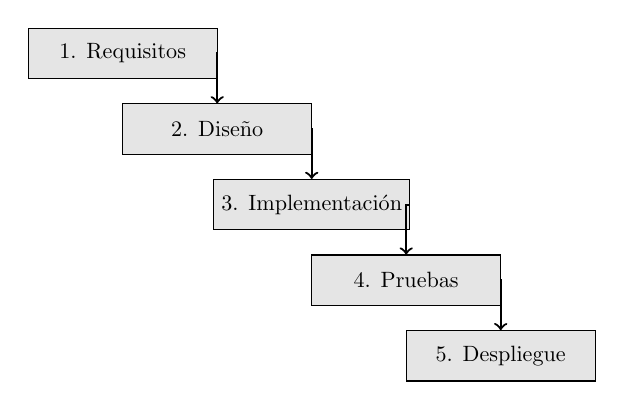
\begin{tikzpicture}[node distance=1.2cm, auto, scale=0.8, transform shape]
    \node (req) [draw, rectangle, minimum width=3cm, minimum height=0.8cm, fill=gray!20] {1. Requisitos};
    \node (dis) [draw, rectangle, minimum width=3cm, minimum height=0.8cm, fill=gray!20, below of=req, xshift=1.5cm] {2. Diseño};
    \node (imp) [draw, rectangle, minimum width=3cm, minimum height=0.8cm, fill=gray!20, below of=dis, xshift=1.5cm] {3. Implementación};
    \node (pru) [draw, rectangle, minimum width=3cm, minimum height=0.8cm, fill=gray!20, below of=imp, xshift=1.5cm] {4. Pruebas};
    \node (des) [draw, rectangle, minimum width=3cm, minimum height=0.8cm, fill=gray!20, below of=pru, xshift=1.5cm] {5. Despliegue};
    
    \draw[->, thick] (req.east) -| (dis.north);
    \draw[->, thick] (dis.east) -| (imp.north);
    \draw[->, thick] (imp.east) -| (pru.north);
    \draw[->, thick] (pru.east) -| (des.north);
\end{tikzpicture}
\captionof{figure}{Modelo de Desarrollo en Cascada}
\end{center}
\vspace{0.5cm}
\newpage
\subsubsection{Scrum}
\textbf{Enfoque:} Metodología ágil que se basa en el desarrollo iterativo e incremental. Opera bajo el empirismo, permitiendo una rápida adaptación a los cambios y promoviendo la entrega continua de valor. El trabajo se divide en iteraciones cortas y de tiempo fijo llamadas Sprints \citep{schwaber2020scrum}.

\textbf{Fases o Etapas:}
\begin{enumerate}
    \item \textit{Product Backlog:} Lista priorizada de todos los requisitos del proyecto.
    \item \textit{Sprint Planning:} Reunión para definir qué elementos se desarrollarán.
    \item \textit{Sprint (Ejecución):} Periodo de desarrollo con reuniones diarias (\textit{Daily Scrum}).
    \item \textit{Sprint Review:} Demostración del incremento de software desarrollado.
    \item \textit{Sprint Retrospective:} Análisis interno para mejora continua.
\end{enumerate}

\textbf{Representación Gráfica:}
\vspace{0.5cm}
\begin{center}
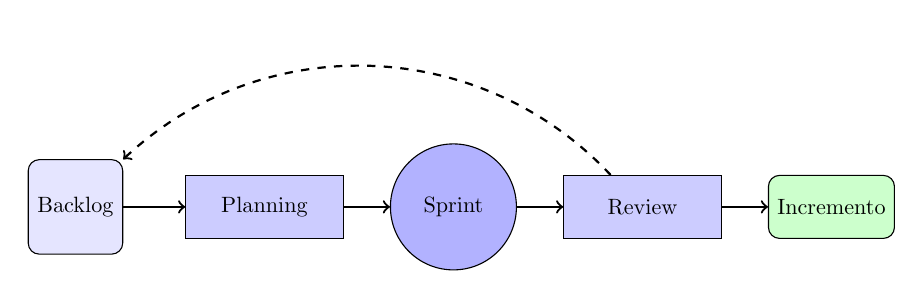
\begin{tikzpicture}[node distance=2.5cm, auto, scale=0.8, transform shape]
    \node (backlog) [draw, rectangle, rounded corners, minimum height=1.5cm, minimum width=1.5cm, fill=blue!10] {Backlog};
    \node (sprintplan) [draw, rectangle, minimum width=2.5cm, minimum height=1cm, fill=blue!20, right of=backlog, node distance=3cm] {Planning};
    \node (sprint) [draw, circle, minimum size=2cm, fill=blue!30, right of=sprintplan, node distance=3cm] {Sprint};
    \node (review) [draw, rectangle, minimum width=2.5cm, minimum height=1cm, fill=blue!20, right of=sprint, node distance=3cm] {Review};
    \node (inc) [draw, rectangle, rounded corners, minimum width=2cm, minimum height=1cm, fill=green!20, right of=review, node distance=3cm] {Incremento};
    
    \draw[->, thick] (backlog) -- (sprintplan);
    \draw[->, thick] (sprintplan) -- (sprint);
    \draw[->, thick] (sprint) -- (review);
    \draw[->, thick] (review) -- (inc);
    \draw[->, thick, dashed] (review) to[bend right=45] (backlog);
\end{tikzpicture}
\captionof{figure}{Ciclo de Vida de Scrum}
\end{center}
\vspace{0.5cm}
\newpage
\subsubsection{Kanban}
\textbf{Enfoque:} Basado en los principios Lean, es un marco ágil centrado en la visualización del flujo de trabajo y la entrega continua, regulando el ritmo mediante la limitación del Trabajo en Progreso (WIP) sin imponer Sprints de tiempo fijo \citep{anderson2010kanban}.

\textbf{Fases o Prácticas Principales:}
\begin{enumerate}
    \item \textit{Visualización del flujo:} Mapeo del proceso (ej. Por Hacer, En Desarrollo, Pruebas, Hecho).
    \item \textit{Límites de WIP (Work in Progress):} Restricción de tareas simultáneas por columna.
    \item \textit{Gestión del flujo:} Monitoreo para resolver bloqueos rápidamente.
    \item \textit{Mejora colaborativa:} Optimización continua del proceso.
\end{enumerate}

\textbf{Representación Gráfica:}
\vspace{0.5cm}
\begin{center}
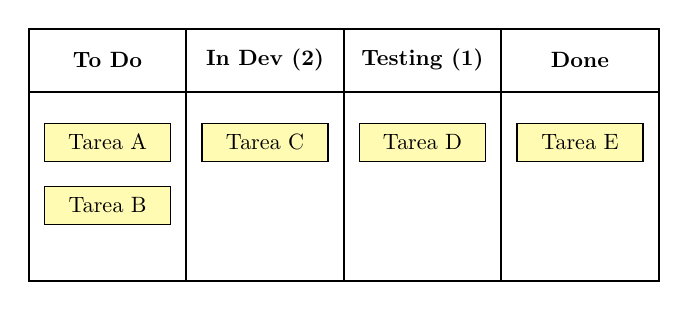
\begin{tikzpicture}[scale=0.8, transform shape]
    % Tablero
    \draw[thick] (0,0) rectangle (10,4);
    \draw[thick] (2.5,0) -- (2.5,4);
    \draw[thick] (5,0) -- (5,4);
    \draw[thick] (7.5,0) -- (7.5,4);
    
    % Cabeceras
    \node at (1.25, 3.5) {\textbf{To Do}};
    \node at (3.75, 3.5) {\textbf{In Dev (2)}};
    \node at (6.25, 3.5) {\textbf{Testing (1)}};
    \node at (8.75, 3.5) {\textbf{Done}};
    \draw[thick] (0,3) -- (10,3);
    
    % Tarjetas
    \node[draw, fill=yellow!30, minimum width=2cm, minimum height=0.6cm] at (1.25, 2.2) {Tarea A};
    \node[draw, fill=yellow!30, minimum width=2cm, minimum height=0.6cm] at (1.25, 1.2) {Tarea B};
    \node[draw, fill=yellow!30, minimum width=2cm, minimum height=0.6cm] at (3.75, 2.2) {Tarea C};
    \node[draw, fill=yellow!30, minimum width=2cm, minimum height=0.6cm] at (6.25, 2.2) {Tarea D};
    \node[draw, fill=yellow!30, minimum width=2cm, minimum height=0.6cm] at (8.75, 2.2) {Tarea E};
\end{tikzpicture}
\captionof{figure}{Tablero Kanban Básico}
\end{center}
\vspace{0.5cm}
\newpage
\subsection{Evaluación de Alternativas}
Para determinar qué metodología es más apta para el desarrollo de la aplicación descrita, se evaluaron los tres enfoques con base en los siguientes criterios de análisis:

\begin{itemize}
    \item \textbf{Aplicabilidad:} Idoneidad para proyectos con alto nivel de innovación tecnológica, integración de APIs y algoritmos predictivos.
    \item \textbf{Eficiencia:} Capacidad de generar entregables y prototipos funcionales de forma temprana.
    \item \textbf{Costo / Gestión de Riesgos:} Facilidad para mitigar riesgos o redirigir esfuerzos sin un alto impacto financiero.
    \item \textbf{Calidad:} Enfoque en la validación constante, pruebas con usuarios y retroalimentación oportuna.
    \item \textbf{Adaptabilidad:} Flexibilidad para incorporar cambios en los requisitos en etapas avanzadas.
\end{itemize}
\newpage
\subsection{Cuadro Comparativo}
A continuación, se presenta un resumen cualitativo comparando las metodologías estudiadas frente a los requerimientos y la naturaleza del proyecto.

\begin{table}[h!]
    \centering
    \renewcommand{\arraystretch}{1.5}
    \begin{tabular}{|m{2.7cm}|m{4cm}|m{4cm}|m{4cm}|}
        \hline
        \rowcolor[HTML]{EFEFEF}
        \textbf{Criterio} & \textbf{Cascada (Waterfall)} & \textbf{Scrum (Ágil)} & \textbf{Kanban (Lean/Ágil)} \\ \hline
        \textbf{Aplicabilidad} & Baja. No soporta bien la incertidumbre de integrar nuevos modelos de IA. & Alta. Permite probar y validar integraciones en iteraciones cortas. & Alta. El flujo continuo permite incorporar cambios día a día. \\ \hline
        \textbf{Eficiencia} & Baja. El software funcional se obtiene al final del ciclo. & Alta. Genera incrementos funcionales periódicos. & Media-Alta. Entrega continua enfocada en reducir cuellos de botella. \\ \hline
        \textbf{Costo / Riesgos} & Alto riesgo. Corregir fallos arquitectónicos tardíos es costoso. & Bajo riesgo. Los errores se detectan en iteraciones tempranas. & Bajo riesgo. Visualización inmediata de bloqueos. \\ \hline
        \textbf{Calidad} & Validaciones concentradas al final del ciclo. & Validaciones constantes en cada \textit{Sprint Review}. & Alta calidad por la restricción del trabajo en curso (WIP). \\ \hline
        \textbf{Adaptabilidad} & Muy baja. Resistente a cambios de requisitos. & Alta. Los requerimientos pueden ajustarse entre Sprints. & Muy Alta. Priorización dinámica y adaptación continua. \\ \hline
    \end{tabular}
    \caption{Cuadro comparativo de alternativas metodológicas.}
    \label{tab:comparativa_metodologias}
\end{table}
\newpage
\subsection{Justificación Metodología Seleccionada}

Tras evaluar las alternativas expuestas, se concluye que la adopción de una metodología "de libro" ---ya sea tradicional o ágil--- no se ajusta de manera óptima a la realidad de este proyecto de ingeniería. Por un lado, el desarrollo en Cascada es inviable debido a la incertidumbre técnica inherente a la integración de telemetría de dispositivos de terceros y al ajuste de modelos predictivos de fatiga cruzada. Por otro lado, la implementación de un marco de trabajo como \textit{Scrum} en su estado puro puede resultar excesivamente rígida para el equipo de desarrollo frente a las fases de investigación y desarrollo (I+D) que exige el proyecto. La integración de tecnologías emergentes, el consumo de APIs de terceros y el entrenamiento de algoritmos predictivos a menudo presentan bloqueos imprevistos que dificultan estimar con exactitud la capacidad de trabajo en un \textit{Sprint} cerrado. Forzar esta estructura estática puede derivar en una burocratización ineficiente de las ceremonias del equipo, restando foco a la resolución de problemas técnicos complejos.
\\\\
Por consiguiente, para este proyecto se ha seleccionado una \textbf{Metodología Ágil Híbrida Adaptada (Scrumban con enfoque Lean UX)}. Esta decisión se fundamenta en extraer las prácticas que mayor valor y agilidad aportan al desarrollo del sistema:
\begin{itemize}
    \item \textbf{De Scrum:} Se adoptará el trabajo mediante iteraciones cortas (ciclos o \textit{Sprints} de 2 a 3 semanas) y la ceremonia de revisión (\textit{Sprint Review}). Esto garantiza la generación progresiva de incrementos de software funcional, estableciendo hitos de control periódicos.
    \item \textbf{De Kanban:} Se utilizará la gestión visual del flujo de trabajo y la limitación estricta del Trabajo en Progreso (WIP). Al enfrentarse a desafíos técnicos complejos (como el consumo de APIs de salud o la implementación de Procesamiento de Lenguaje Natural), el enfoque de flujo continuo permite flexibilizar los tiempos de desarrollo de una tarea crítica sin la presión de "fracasar" un Sprint estático.
    \item \textbf{Del enfoque Lean / Design Thinking:} Considerando que el problema central identificado en el Capítulo 2 es la fricción operativa que sufren los atletas con las aplicaciones actuales, se integrará una capa de validación mediante prototipado rápido antes de la codificación.
\end{itemize}
\newpage
\subsection{Diseño del Plan Metodológico del Proyecto}

La Metodología Ágil Híbrida definida se estructurará a través de un ciclo de vida iterativo e incremental. El proceso de construcción de la plataforma constará de cinco fases principales, las cuales se repetirán hasta alcanzar el Producto Mínimo Viable (MVP) y sus versiones maduras:

\begin{enumerate}
    \item \textbf{Fase 1: Ideación y Prototipado Rápido (Enfoque Lean UX):}
    Previo a la codificación de módulos complejos (como el recomendador dinámico de nutrición o el \textit{dashboard} adaptativo), se diseñarán prototipos de alta fidelidad de las interfaces. Estos flujos de pantalla serán validados para garantizar que la lógica de prevención de interferencia en el entrenamiento concurrente se presenta de manera intuitiva y reduce la fricción de entrada de datos.
    
    \item \textbf{Fase 2: Planificación de la Iteración (Basado en Scrum):}
    Al inicio de cada iteración, se seleccionarán los requerimientos prioritarios desde la Pila del Producto (\textit{Product Backlog}) para conformar los objetivos técnicos del ciclo. En esta etapa se definirán arquitecturas preliminares de bases de datos o servicios requeridos para dichas características.
    
    \item \textbf{Fase 3: Desarrollo en Flujo Continuo (Basado en Kanban):}
    La codificación e implementación de la arquitectura se gestionará mediante un tablero Kanban (Por Hacer, En Desarrollo, Pruebas y Terminado). Se aplicará una limitación del WIP para asegurar que el equipo no aborde múltiples componentes pesados (por ejemplo, el módulo de telemetría cardiovascular y el motor de Procesamiento de Lenguaje Natural) de forma simultánea, optimizando el rendimiento colectivo, evitando cuellos de botella y aislando los errores con mayor rapidez.
    
    \item \textbf{Fase 4: Pruebas e Integración Técnica:}
    Fase técnica dedicada a someter a prueba la interoperabilidad del sistema. Se verificarán las integraciones y sincronización pasiva con los concentradores de datos externos (por ejemplo, simular el consumo de datos desde un \textit{wearable}), y se realizarán pruebas unitarias para asegurar que los algoritmos de nutrición dinámica escalen correctamente los macronutrientes frente al gasto energético recibido.
    
    \item \textbf{Fase 5: Revisión del Incremento y Ajuste:}
    Al finalizar el ciclo de iteración, se consolidará un entregable funcional que demuestre una nueva característica operativa del sistema. A partir de la retroalimentación obtenida tras su evaluación, se actualizará el \textit{Product Backlog}, refinando los requerimientos técnicos y mitigando riesgos para el inicio de la siguiente iteración.
\end{enumerate}
\subsection{Comentarios Generales del Capítulo}

A modo de síntesis, la definición del marco metodológico representa un pilar fundamental para estructurar el trabajo y mitigar la incertidumbre inherente a este proyecto de ingeniería. Al descartar modelos tradicionales rígidos en favor de un Enfoque Ágil Híbrido (Scrumban + Lean UX), se ha dotado al equipo de desarrollo de la flexibilidad necesaria para afrontar con éxito las fases de investigación y desarrollo (I+D), tales como la integración pasiva de telemetría de \textit{wearables} y la formulación de algoritmos de nutrición dinámica. Esta estructura no solo garantiza una gestión eficiente de los recursos y la prevención de cuellos de botella mediante la limitación del trabajo en progreso (WIP), sino que también asegura una alineación constante con las necesidades de los atletas híbridos gracias al prototipado temprano. Establecida esta base operativa de trabajo, en las siguientes secciones se abordarán las distintas alternativas arquitectónicas y los estudios de factibilidad técnica, económica y operativa que permitirán llevar esta propuesta metodológica a la práctica.
\newpage
\section{Alternativas de Solución}
\subsection{Introducción del Capítulo}
Establecida la base metodológica del proyecto, la presente sección tiene como objetivo desglosar las distintas alternativas arquitectónicas y funcionales evaluadas para materializar la solución tecnológica propuesta. Cada alternativa representa un nivel de complejidad integral diferente, abarcando no solo la captura de datos cardiovasculares ---que constituye el componente de mayor variabilidad técnica--- sino también el alcance de las funcionalidades de registro nutricional, asistencia por inteligencia artificial y la profundidad del motor de cruce de datos.
\\\\
Es importante destacar que las tres alternativas comparten una base tecnológica común y un motor de cruce de datos fundamentado en la misma lógica temporal. Lo que varía entre ellas es el volumen y la calidad de los datos de entrada que alimentan dicho motor, impactando directamente en la precisión de las predicciones de fatiga cruzada.
\subsection{Descripción de Alternativas}
\subsubsection{Base Tecnológica Común}

Independientemente de la alternativa seleccionada, la solución se construirá sobre el siguiente \textit{stack} tecnológico compartido:

\begin{itemize}
    \item \textbf{Frontend Móvil:} Flutter (Dart), framework multiplataforma que permite generar aplicaciones nativas para Android e iOS desde una única base de código, reduciendo los tiempos de desarrollo y mantenimiento.
    \item \textbf{Backend / API:} NestJS (Node.js con TypeScript), framework progresivo para la construcción de aplicaciones del lado del servidor. Su arquitectura modular facilita la escalabilidad y la separación de responsabilidades entre los distintos módulos del sistema (nutrición, fuerza, cardio, analítica).
    \item \textbf{Base de Datos:} PostgreSQL con uso extensivo de campos \texttt{JSONB}. Esta elección permite combinar la robustez y consistencia transaccional de una base de datos relacional con la flexibilidad de almacenar documentos semiestructurados. Los registros de sesiones de entrenamiento, comidas y telemetría se almacenarán como documentos JSON dentro de columnas \texttt{JSONB}, lo que permite consultas indexadas sobre datos con estructuras heterogéneas (por ejemplo, una sesión de fuerza con 4 ejercicios versus otra con 7).
\end{itemize}

\textbf{Motor de Cruce de Datos Basado en Timestamps}
\\\\
El diferenciador central de la plataforma es su capacidad de cruzar los datos provenientes de los tres pilares (fuerza, resistencia y nutrición) para ofrecer analítica predictiva sobre la fatiga cruzada. Este motor opera bajo una lógica temporal unificada: cada evento registrado en el sistema (comida, sesión de fuerza, sesión de cardio, reporte de sensaciones) porta una marca temporal precisa (\textit{timestamp}). A partir de estas marcas, el motor calcula:

\begin{enumerate}
    \item \textbf{Ventanas de recuperación:} Tiempo transcurrido entre el fin de una sesión de fuerza y el inicio de la siguiente sesión de cardio (y viceversa). Compara estos intervalos contra los umbrales recomendados por la literatura (6 a 8 horas mínimas entre sesiones de distintas modalidades) para alertar sobre riesgo de interferencia.
    \item \textbf{Adherencia nutricional temporal:} Verifica si las comidas fueron consumidas dentro de las ventanas óptimas relativas al entrenamiento (por ejemplo, ingesta de carbohidratos 2-3 horas antes del cardio, proteínas dentro de las 2 horas posteriores a la fuerza, o si los alimentos se consumieron en el momento adecuado durante una ruta larga).
    \item \textbf{Fatiga acumulada semanal:} Suma progresiva del volumen de entrenamiento en ventanas móviles de 7 días. Para fuerza se calcula como $\sum(\text{series} \times \text{repeticiones} \times \text{peso})$; para cardio, la métrica depende de la alternativa (distancia $\times$ RPE en la más básica, o carga basada en zonas cardíacas y potencia en las más avanzadas).
    \item \textbf{Detección de patrones de interferencia:} Si días consecutivos muestran secuencias de fuerza $\rightarrow$ cardio (o viceversa) con recuperación insuficiente, el sistema emite una alerta y sugiere reestructurar el calendario.
\end{enumerate}

La lógica del motor es \textbf{idéntica} en las tres alternativas. Lo que varía es la \textbf{calidad y granularidad de los datos de entrada}: con más capas de información (frecuencia cardíaca, potencia, cadencia), el motor produce predicciones más precisas.

\subsubsection{Alternativa 1: Solución Minimalista (MVP Lean)}

\textbf{Descripción General}
\\\\
Esta alternativa representa el nivel mínimo de funcionalidad viable para abordar la problemática del entrenamiento concurrente. Se orienta a minimizar los costos de desarrollo y el tiempo de entrega, sacrificando la automatización avanzada y la precisión de los biomarcadores en favor de la simplicidad operativa. La propuesta está diseñada para usuarios que no poseen \textit{wearables} y que están dispuestos a realizar un registro manual de su actividad.
\\\\
\textbf{Módulo de Nutrición}
\\\\
El registro de alimentos se realiza exclusivamente mediante formularios manuales. El usuario selecciona ingredientes desde una base de datos local alimentada por una API gratuita de alimentos (como OpenFoodFacts) e ingresa las cantidades consumidas. El sistema calcula automáticamente los macronutrientes y calorías de cada comida. No se incorpora inteligencia artificial para la estimación nutricional mediante fotografías ni procesamiento de lenguaje natural.
\\\\
\textbf{Módulo de Fuerza}
\\\\
El usuario crea rutinas base (plantillas de ejercicios) y registra cada sesión mediante formularios estructurados: selecciona el ejercicio, ingresa series, repeticiones y peso. Incluye un campo de texto libre para describir sensaciones subjetivas asociadas a cada ejercicio. No se implementa registro asistido por PLN.
\newpage
\textbf{Módulo de Cardio}
\\\\
El registro cardiovascular se limita al sensor GPS del teléfono móvil y a la percepción subjetiva del esfuerzo (RPE). La aplicación graba la ruta, velocidad, distancia y tiempo utilizando los servicios de ubicación del dispositivo. Al finalizar la sesión, el usuario registra su RPE en una escala estandarizada (1 a 10) y puede agregar notas de sensaciones. No existe integración con \textit{wearables}, \textit{Health Connect}, \textit{Apple Health} ni archivos \texttt{.fit}.
\\\\
\textbf{Motor de Cruce de Datos}
\\\\
El motor de cruce temporal opera con datos limitados. La fatiga cardiovascular se estima a partir de la distancia recorrida, el tiempo y el RPE reportado. Al carecer de datos de frecuencia cardíaca, el modelo no puede determinar las zonas de entrenamiento ni el gasto calórico real, por lo que las predicciones de fatiga cruzada constituyen aproximaciones basadas en el volumen declarado.
\\\\
\textbf{Módulo Social}
\\\\
Se implementa una funcionalidad básica de comunidad donde los usuarios pueden compartir rutas, rutinas de fuerza y recetas. No incluye escalado automático de porciones.
\\\\
\textbf{Arquitectura de la Solución}
\\\\
La arquitectura de esta alternativa es monolítica y sencilla. El cliente móvil (Flutter) consume directamente una API REST servida por NestJS, la cual gestiona toda la lógica de negocio y persiste los datos en PostgreSQL.

\vspace{0.5cm}
\begin{center}
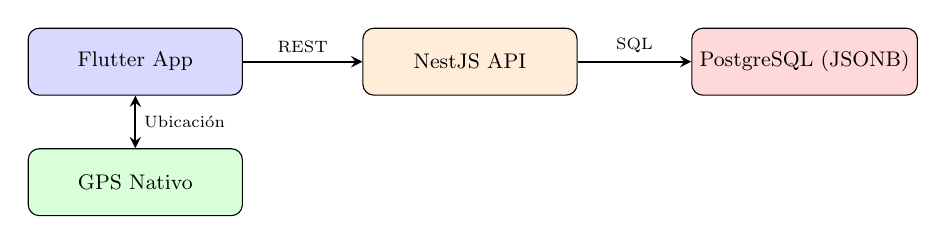
\begin{tikzpicture}[
    node distance=1.8cm,
    box/.style={draw, rectangle, rounded corners, minimum width=3.2cm, minimum height=1cm, fill=#1, text centered, font=\small},
    arrow/.style={->, thick, >=stealth},
    scale=0.85, transform shape
]
    % Frontend
    \node (app) [box=blue!15] {Flutter App};
    \node (gps) [box=green!15, below of=app] {GPS Nativo};

    % Backend
    \node (api) [box=orange!15, right of=app, node distance=5cm] {NestJS API};

    % Database
    \node (db) [box=red!15, right of=api, node distance=5cm] {PostgreSQL (JSONB)};

    % Arrows
    \draw[arrow] (app) -- node[above, font=\scriptsize] {REST} (api);
    \draw[arrow] (api) -- node[above, font=\scriptsize] {SQL} (db);
    \draw[arrow, <->] (app) -- node[right, font=\scriptsize] {Ubicación} (gps);

\end{tikzpicture}
\captionof{figure}{Arquitectura de la Alternativa 1: Solución Minimalista.}
\end{center}
\vspace{0.5cm}

\textbf{Estimación de Costos y Tiempos}
\\\\
La siguiente tabla presenta la estimación de costos para el desarrollo e implementación de esta alternativa, considerando un único desarrollador y tarifas de referencia del mercado chileno para perfiles junior-medio.

\begin{table}[h!]
    \centering
    \renewcommand{\arraystretch}{1.4}
    \begin{tabular}{|m{4cm}|m{5.5cm}|r|}
        \hline
        \rowcolor[HTML]{EFEFEF}
        \textbf{Ítem} & \textbf{Detalle} & \textbf{Costo (CLP)} \\ \hline
        Desarrollo Frontend & Formularios, GPS, UI básica (~200h $\times$ \$15.000/h) & \$3.000.000 \\ \hline
        Desarrollo Backend & API REST, autenticación, CRUD (~150h $\times$ \$15.000/h) & \$2.250.000 \\ \hline
        Base de Datos y DevOps & Schema, migraciones, despliegue (~50h $\times$ \$15.000/h) & \$750.000 \\ \hline
        Testing y QA & Pruebas unitarias e integración (~100h $\times$ \$15.000/h) & \$1.500.000 \\ \hline
        Infraestructura Cloud & VPS + PostgreSQL gestionado (12 meses $\times$ \$30.000/mes) & \$360.000 \\ \hline
        Publicación & Google Play (\$25 USD) + Apple Developer (\$99 USD/año) & \$120.000 \\ \hline
        \rowcolor[HTML]{E8F5E9}
        \textbf{Total Estimado} & \textbf{~500 horas de desarrollo | 3-4 meses} & \textbf{\$7.980.000} \\ \hline
    \end{tabular}
    \caption{Estimación de costos de la Alternativa 1: Solución Minimalista.}
    \label{tab:costos_alt1}
\end{table}

\newpage
\subsubsection{Alternativa 2: Solución Integrada con Brokers del Sistema Operativo}

\textbf{Descripción General}
\\\\
Esta alternativa representa el estándar adoptado por la industria actual de aplicaciones deportivas. Delega la captura de telemetría pesada a los dispositivos \textit{wearables} del usuario y consume los datos de forma pasiva a través de los concentradores nativos del sistema operativo: \textbf{Health Connect} en Android y \textbf{Apple Health (HealthKit)} en iOS. Además, incorpora inteligencia artificial para reducir la fricción en el registro de alimentos y rutinas de fuerza.
\\\\
\textbf{Módulo de Nutrición}
\\\\
El registro de alimentos se realiza mediante dos vías asistidas por inteligencia artificial:
\begin{itemize}
    \item \textbf{Procesamiento de Lenguaje Natural (PLN):} El usuario describe su comida en lenguaje cotidiano (por ejemplo, ``desayuné 3 huevos con avena y yogurt'') y el sistema estructura automáticamente los ingredientes y estima los macronutrientes.
    \item \textbf{Visión Artificial:} El usuario puede fotografiar su plato y un modelo de ML estima los alimentos presentes y sus cantidades aproximadas, permitiendo la edición posterior.
\end{itemize}
Ambas funcionalidades consumen una API de inferencia en la nube (como Gemini API o un modelo equivalente). Se mantiene la base de datos de alimentos para validación y corrección.
\\\\
\textbf{Módulo de Fuerza}
\\\\
Además del formulario estructurado, se incorpora el registro asistido por PLN: el usuario puede dictar o escribir su rutina en lenguaje natural (por ejemplo, ``hice 3 series de 10 sentadillas con 80 kilos'') y el sistema extrae automáticamente el ejercicio, series, repeticiones y peso, estructurando la información en la base de datos. Se mantiene el registro de sensaciones subjetivas vinculado a cada ejercicio.
\\\\
\textbf{Módulo de Cardio}
\\\\
El sistema consume pasivamente los datos centralizados por \textit{Health Connect} (Android) y \textit{Apple Health} (iOS). Cuando el usuario finaliza una sesión de cardio registrada en cualquier \textit{wearable} compatible (Garmin, Polar, Apple Watch, Samsung Galaxy Watch, entre otros), los datos se sincronizan automáticamente al concentrador del SO, y la aplicación los importa en segundo plano. Las métricas disponibles a través de los \textit{brokers} incluyen:

\begin{itemize}
    \item Frecuencia cardíaca promedio y máxima de la sesión.
    \item Calorías activas estimadas por el dispositivo.
    \item Distancia recorrida y duración.
    \item Ruta GPS (cuando el \textit{wearable} la registra).
    \item Zonas de ritmo cardíaco (calculadas por la aplicación a partir de la FC importada).
\end{itemize}

Adicionalmente, se mantiene el GPS nativo del teléfono como respaldo para usuarios sin \textit{wearable}, complementado con el RPE.
\\\\
\textbf{Motor de Cruce de Datos}
\\\\
Con la incorporación de la frecuencia cardíaca y las calorías activas reales, el motor de cruce temporal opera con mayor precisión. Puede determinar las zonas de entrenamiento cardiovascular (Zona 1 a Zona 5) y calcular el gasto calórico diferenciado, permitiendo al módulo de nutrición dinámica ajustar los macronutrientes con base en el sustrato energético predominante (carbohidratos en zonas altas, grasas en zonas bajas). Las predicciones de fatiga cruzada ganan en confiabilidad al incorporar la carga interna (estrés cardíaco) además de la carga externa (volumen y distancia).
\\\\
\textbf{Módulo Social}
\\\\
Se implementa la comunidad con la capacidad de compartir rutas, rutinas y recetas. Se incorpora el escalado automático de porciones: el motor toma una receta de la comunidad y ajusta matemáticamente las cantidades de ingredientes para cubrir los macronutrientes objetivo del usuario según el desgaste del día.
\\\\
\textbf{Arquitectura de la Solución}
\\\\
La arquitectura incorpora la capa de integración con los SDKs nativos de \textit{Health Connect} y \textit{HealthKit}, además de un servicio de inferencia de IA en la nube para el procesamiento de lenguaje natural y visión artificial.

\vspace{0.5cm}
\begin{center}
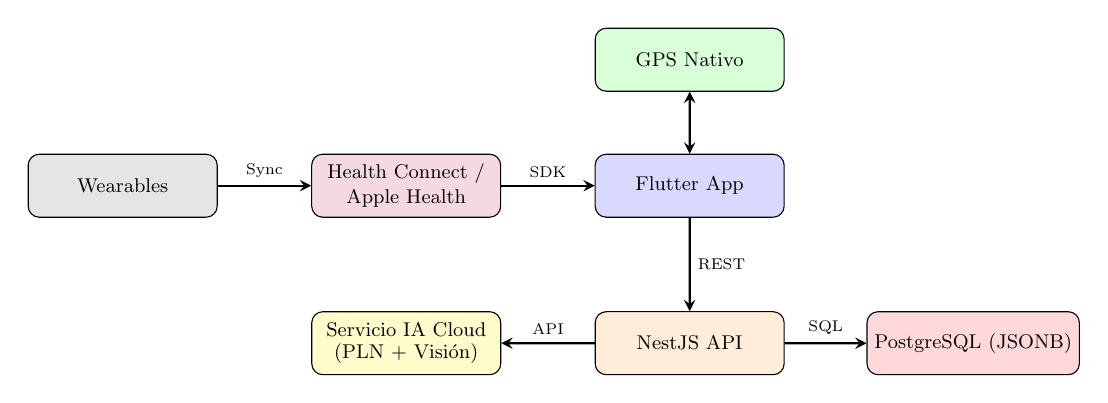
\begin{tikzpicture}[
    node distance=2cm,
    box/.style={draw, rectangle, rounded corners, minimum width=3cm, minimum height=1cm, fill=#1, text centered, font=\small},
    arrow/.style={->, thick, >=stealth},
    darrow/.style={<->, thick, >=stealth},
    scale=0.8, transform shape
]
    % External devices
    \node (wear) [box=gray!20] {Wearables};
    \node (hc) [box=purple!15, right of=wear, node distance=4.5cm] {\shortstack{Health Connect /\\Apple Health}};

    % Frontend
    \node (app) [box=blue!15, right of=hc, node distance=4.5cm] {Flutter App};

    % Backend
    \node (api) [box=orange!15, below of=app, node distance=2.5cm] {NestJS API};

    % AI Service
    \node (ai) [box=yellow!20, left of=api, node distance=4.5cm] {\shortstack{Servicio IA Cloud\\(PLN + Visión)}};

    % Database
    \node (db) [box=red!15, right of=api, node distance=4.5cm] {PostgreSQL (JSONB)};

    % GPS
    \node (gps) [box=green!15, above of=app, node distance=2cm] {GPS Nativo};

    % Arrows
    \draw[arrow] (wear) -- node[above, font=\scriptsize] {Sync} (hc);
    \draw[arrow] (hc) -- node[above, font=\scriptsize] {SDK} (app);
    \draw[arrow] (app) -- node[right, font=\scriptsize] {REST} (api);
    \draw[arrow] (api) -- node[above, font=\scriptsize] {SQL} (db);
    \draw[arrow] (api) -- node[above, font=\scriptsize] {API} (ai);
    \draw[darrow] (gps) -- node[right, font=\scriptsize] {} (app);

\end{tikzpicture}
\captionof{figure}{Arquitectura de la Alternativa 2: Solución Integrada con Brokers del SO.}
\end{center}
\vspace{0.5cm}
\newpage
\textbf{Estimación de Costos y Tiempos}

\begin{table}[h!]
    \centering
    \renewcommand{\arraystretch}{1.4}
    \begin{tabular}{|m{4cm}|m{5.5cm}|r|}
        \hline
        \rowcolor[HTML]{EFEFEF}
        \textbf{Ítem} & \textbf{Detalle} & \textbf{Costo (CLP)} \\ \hline
        Desarrollo Frontend & UI completa, PLN, cámara, SDK Health (~350h $\times$ \$15.000/h) & \$5.250.000 \\ \hline
        Desarrollo Backend & API REST, módulos IA, motor nutrición (~280h $\times$ \$15.000/h) & \$4.200.000 \\ \hline
        Integración Brokers & Health Connect + HealthKit, testing cross-platform (~120h $\times$ \$15.000/h) & \$1.800.000 \\ \hline
        Base de Datos y DevOps & Schema, migraciones, CI/CD (~80h $\times$ \$15.000/h) & \$1.200.000 \\ \hline
        Testing y QA & Pruebas unitarias, integración, dispositivos (~120h $\times$ \$15.000/h) & \$1.800.000 \\ \hline
        Infraestructura Cloud & VPS + PostgreSQL (12 meses $\times$ \$50.000/mes) & \$600.000 \\ \hline
        APIs de IA & Gemini / OpenAI (12 meses $\times$ \$30.000/mes) & \$360.000 \\ \hline
        Publicación & Google Play + Apple Developer & \$120.000 \\ \hline
        \rowcolor[HTML]{E8F5E9}
        \textbf{Total Estimado} & \textbf{~950 horas de desarrollo | 6-7 meses} & \textbf{\$15.330.000} \\ \hline
    \end{tabular}
    \caption{Estimación de costos de la Alternativa 2: Solución Integrada con Brokers.}
    \label{tab:costos_alt2}
\end{table}

\textbf{Limitación crítica:} Los concentradores del sistema operativo tienden a resumir y filtrar la información proveniente de los \textit{wearables}. Variables técnicas avanzadas del ciclismo, como la potencia real del pedal (vatios), la cadencia de pedaleo o los datos segundo a segundo, habitualmente no se exponen a través de \textit{Health Connect} ni \textit{Apple Health}. Esto limita la precisión del análisis para ciclistas que entrenan con potenciómetros o ciclocomputadores avanzados.

\newpage
\subsubsection{Alternativa 3: Solución por Capas (Ecosistema Flexible)}

\textbf{Descripción General}
\\\\
Esta alternativa unifica las anteriores en un ecosistema flexible que consume distintas fuentes de datos según el nivel de equipamiento del deportista. El sistema procesa la información de forma jerárquica mediante tres capas, garantizando que el motor de cruce siempre disponga de un piso mínimo de datos (GPS + RPE) para estimar la fatiga, pero permitiendo escalar hacia un análisis de alta precisión cuando el usuario proporciona datos desde su ciclocomputador o \textit{smartwatch}.
\\\\
\textbf{Módulo de Nutrición}
\\\\
Incorpora todas las funcionalidades de la Alternativa 2 (PLN + visión artificial) y añade el módulo comunitario con escalado automático de recetas. El motor de escalado analiza los macronutrientes objetivo del usuario (calculados dinámicamente según la sesión del día) y ajusta las cantidades de cada ingrediente de una receta compartida para cubrir exactamente los requerimientos.
\\\\
\textbf{Módulo de Fuerza}
\\\\
Idéntico a la Alternativa 2: formulario estructurado + PLN (voz/texto) + registro de sensaciones subjetivas vinculadas a cada ejercicio y serie.
\newpage
\textbf{Módulo de Cardio: Sistema de Tres Capas}

\begin{itemize}
    \item \textbf{Capa Base (Sin hardware externo):} La aplicación captura la ruta mediante el GPS del teléfono y exige un reporte de RPE y sensaciones subjetivas al finalizar la sesión. El motor de cruce opera con métricas de volumen externo (distancia, velocidad, tiempo) y percepción.
    \item \textbf{Capa Intermedia (Automatización pasiva):} Si el usuario vincula un \textit{smartwatch}, el sistema extrae la frecuencia cardíaca, las calorías activas y los registros de sueño desde los \textit{brokers} del SO (\textit{Health Connect} / \textit{Apple Health}) de manera transparente. El motor de cruce incorpora las zonas cardíacas y el gasto calórico real, mejorando la precisión de las predicciones.
    \item \textbf{Capa Avanzada (Máxima granularidad):} Para el ciclista que utiliza un ciclocomputador, la aplicación ofrece un apartado de importación de archivos \texttt{.fit}. El \textit{backend} procesa estos archivos mediante un servicio de \textit{parsing} dedicado, extrayendo la potencia real del pedal (vatios), cadencia, frecuencia cardíaca segundo a segundo, altimetría detallada y todas las métricas avanzadas que el dispositivo haya registrado. Cuando datos de la capa avanzada están disponibles, el sistema les da \textbf{prioridad}, sobrescribiendo los datos resumidos provenientes de las capas inferiores para ese mismo evento.
\end{itemize}

\textbf{Motor de Cruce de Datos}
\\\\
El motor de cruce opera de forma adaptativa. Mantiene un indicador de \textbf{confianza} para cada sesión de cardio, el cual refleja la capa de datos con la que fue registrada:
\begin{itemize}
    \item \textit{Confianza baja:} Solo GPS + RPE. Fatiga estimada por volumen externo.
    \item \textit{Confianza media:} GPS + FC (desde \textit{broker}). Fatiga calculada por zonas cardíacas.
    \item \textit{Confianza alta:} Archivo \texttt{.fit} procesado. Fatiga calculada con potencia real, carga TSS (\textit{Training Stress Score}) y análisis metabólico detallado.
\end{itemize}
Este esquema permite que el algoritmo pondere sus predicciones de interferencia y fatiga cruzada según la calidad de la información disponible, evitando falsos positivos en escenarios de datos limitados.
\\\\
\textbf{Módulo Social}
\\\\
Funcionalidad completa: comunidad con publicación de rutas, rutinas y recetas, escalado automático de porciones y visualización de datos compartidos (con consentimiento del usuario).
\\\\
\textbf{Arquitectura de la Solución}
\\\\
La arquitectura se modulariza para soportar las múltiples fuentes de datos. El \textit{backend} NestJS se organiza en módulos especializados que pueden evolucionar de forma independiente: un módulo de \textit{parsing} para archivos \texttt{.fit}, un módulo de nutrición con motor de escalado, y un módulo de analítica de fatiga.

\vspace{0.5cm}
\begin{center}
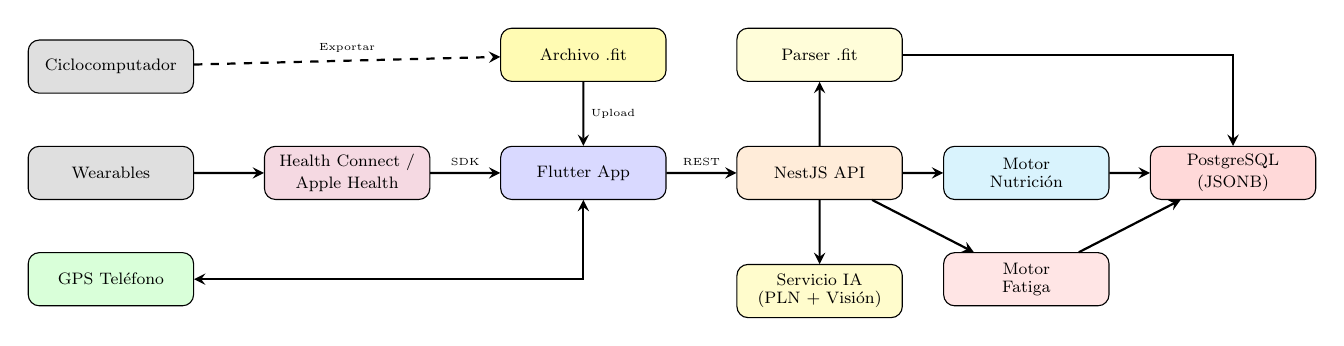
\begin{tikzpicture}[
    node distance=2cm,
    box/.style={draw, rectangle, rounded corners, minimum width=2.8cm, minimum height=0.9cm, fill=#1, text centered, font=\footnotesize},
    arrow/.style={->, thick, >=stealth},
    darrow/.style={<->, thick, >=stealth},
    dashed_arrow/.style={->, dashed, thick, >=stealth},
    scale=0.75, transform shape
]
    % External Layer - Left
    \node (ciclo) [box=gray!25] {Ciclocomputador};
    \node (wear) [box=gray!25, below of=ciclo, node distance=1.8cm] {Wearables};
    \node (gps) [box=green!15, below of=wear, node distance=1.8cm] {GPS Teléfono};

    % Broker Layer
    \node (hc) [box=purple!15, right of=wear, node distance=4cm] {\shortstack{Health Connect /\\Apple Health}};

    % App
    \node (app) [box=blue!15, right of=hc, node distance=4cm] {Flutter App};

    % File upload path
    \node (fit) [box=yellow!30, above of=app, node distance=2cm] {Archivo .fit};

    % Backend
    \node (api) [box=orange!15, right of=app, node distance=4cm] {NestJS API};

    % Backend modules
    \node (parser) [box=yellow!15, above of=api, node distance=2cm] {Parser .fit};
    \node (nutri) [box=cyan!15, right of=api, node distance=3.5cm] {\shortstack{Motor\\Nutrición}};
    \node (fatiga) [box=red!10, below of=nutri, node distance=1.8cm] {\shortstack{Motor\\Fatiga}};

    % AI
    \node (ai) [box=yellow!20, below of=api, node distance=2cm] {\shortstack{Servicio IA\\(PLN + Visión)}};

    % Database
    \node (db) [box=red!15, right of=nutri, node distance=3.5cm] {\shortstack{PostgreSQL\\(JSONB)}};

    % Arrows
    \draw[arrow] (wear) -- (hc);
    \draw[arrow] (hc) -- node[above, font=\tiny] {SDK} (app);
    \draw[darrow] (gps) -| (app);
    \draw[dashed_arrow] (ciclo) -- node[above, font=\tiny] {Exportar} (fit);
    \draw[arrow] (fit) -- node[right, font=\tiny] {Upload} (app);
    \draw[arrow] (app) -- node[above, font=\tiny] {REST} (api);
    \draw[arrow] (api) -- (parser);
    \draw[arrow] (api) -- (nutri);
    \draw[arrow] (api) -- (fatiga);
    \draw[arrow] (api) -- (ai);
    \draw[arrow] (nutri) -- (db);
    \draw[arrow] (fatiga) -- (db);
    \draw[arrow] (parser) -| (db);

\end{tikzpicture}
\captionof{figure}{Arquitectura de la Alternativa 3: Solución por Capas.}
\end{center}
\vspace{0.5cm}
\newpage
\textbf{Estimación de Costos y Tiempos}

\begin{table}[h!]
    \centering
    \renewcommand{\arraystretch}{1.4}
    \begin{tabular}{|m{4cm}|m{5.5cm}|r|}
        \hline
        \rowcolor[HTML]{EFEFEF}
        \textbf{Ítem} & \textbf{Detalle} & \textbf{Costo (CLP)} \\ \hline
        Desarrollo Frontend & UI completa, PLN, cámara, SDK Health, upload .fit (~400h $\times$ \$15.000/h) & \$6.000.000 \\ \hline
        Desarrollo Backend & API modular, motor nutrición, motor fatiga (~350h $\times$ \$15.000/h) & \$5.250.000 \\ \hline
        Parser de archivos .fit & Desarrollo y testing del servicio de parsing (~120h $\times$ \$15.000/h) & \$1.800.000 \\ \hline
        Integración Brokers & Health Connect + HealthKit (~120h $\times$ \$15.000/h) & \$1.800.000 \\ \hline
        Motor de Escalado Social & Recetas + escalado de porciones (~80h $\times$ \$15.000/h) & \$1.200.000 \\ \hline
        Base de Datos y DevOps & Schema flexible, normalización, CI/CD (~100h $\times$ \$15.000/h) & \$1.500.000 \\ \hline
        Testing y QA & Pruebas multi-capa, dispositivos, .fit (~150h $\times$ \$15.000/h) & \$2.250.000 \\ \hline
        Infraestructura Cloud & VPS robusta + PostgreSQL (12 meses $\times$ \$80.000/mes) & \$960.000 \\ \hline
        APIs de IA & Gemini / OpenAI (12 meses $\times$ \$40.000/mes) & \$480.000 \\ \hline
        Publicación & Google Play + Apple Developer & \$120.000 \\ \hline
        \rowcolor[HTML]{E8F5E9}
        \textbf{Total Estimado} & \textbf{~1.320 horas de desarrollo | 9-10 meses} & \textbf{\$21.360.000} \\ \hline
    \end{tabular}
    \caption{Estimación de costos de la Alternativa 3: Solución por Capas.}
    \label{tab:costos_alt3}
\end{table}

\textbf{Complejidad adicional:} Estandarizar registros de cardio provenientes de fuentes con niveles de calidad asimétricos (GPS crudo vs. archivo \texttt{.fit} con miles de puntos por segundo) exige diseñar un esquema de base de datos flexible y un motor de normalización capaz de unificar estos datos heterogéneos en una estructura consultable por el motor de fatiga.
\newpage
\subsubsection{Cuadro Comparativo de Alternativas}
La siguiente tabla sintetiza las diferencias funcionales, técnicas y económicas entre las tres alternativas evaluadas, facilitando la selección fundamentada en el estudio de factibilidad posterior.

\begin{table}[h!]
    \centering
    \renewcommand{\arraystretch}{1.4}
    \begin{tabular}{|m{3.8cm}|m{3.5cm}|m{3.5cm}|m{3.8cm}|}
        \hline
        \rowcolor[HTML]{EFEFEF}
        \textbf{Dimensión} & \textbf{Alt. 1: Minimalista} & \textbf{Alt. 2: Brokers SO} & \textbf{Alt. 3: Por Capas} \\ \hline
        \textbf{Registro Nutricional} & Formulario manual & PLN + Visión IA & PLN + Visión IA + Escalado comunitario \\ \hline
        \textbf{Registro de Fuerza} & Formulario manual & Formulario + PLN & Formulario + PLN \\ \hline
        \textbf{Registro de Cardio} & GPS teléfono + RPE & GPS + Health Connect / Apple Health & GPS + Brokers + Archivo .fit \\ \hline
        \textbf{Frecuencia Cardíaca} & No disponible & Sí (vía broker) & Sí (broker + .fit segundo a segundo) \\ \hline
        \textbf{Potencia (ciclismo)} & No disponible & No disponible & Sí (vía archivo .fit) \\ \hline
        \textbf{Precisión del motor de fatiga} & Baja (volumen + RPE) & Media-Alta (zonas FC + calorías) & Alta (potencia + FC + TSS) \\ \hline
        \textbf{Módulo Social} & Básico (compartir) & Completo (escalado) & Completo (escalado) \\ \hline
        \textbf{Uso de IA} & No & Sí (PLN + Visión) & Sí (PLN + Visión) \\ \hline
        \textbf{Tiempo de desarrollo} & 3-4 meses & 6-7 meses & 9-10 meses \\ \hline
        \textbf{Costo total estimado} & \$7.980.000 CLP & \$15.330.000 CLP & \$21.360.000 CLP \\ \hline
        \textbf{Complejidad técnica} & Baja & Media & Alta \\ \hline
        \textbf{Barrera de entrada usuario} & Ninguna (solo teléfono) & Baja (smartwatch opcional) & Ninguna (escala con hardware) \\ \hline
    \end{tabular}
    \caption{Cuadro comparativo de las alternativas de solución.}
    \label{tab:comparativa_alternativas}
\end{table}
\newpage
\subsection{Estudio de Factibilidad}
El estudio de factibilidad constituye una etapa crítica en la ingeniería de software, cuyo propósito es evaluar y garantizar que la solución propuesta pueda ser materializada de manera exitosa antes de incurrir en la asignación definitiva de recursos. Este análisis se desglosa en tres dimensiones fundamentales: técnica, económica y operativa. A través de esta evaluación sistemática, se busca identificar restricciones, mitigar riesgos tempranos y determinar si se cuenta con las capacidades tecnológicas, el presupuesto y la disposición procedimental para llevar a cabo la construcción del sistema, asegurando que la alternativa escogida (y las tecnologías que la componen) sean viables para el desarrollo del Producto Mínimo Viable (MVP).

\subsubsection{Factibilidad Técnica}
La factibilidad técnica evalúa si se dispone de la tecnología, la infraestructura y los conocimientos necesarios para desarrollar y mantener el sistema. Para este proyecto, considerando el nivel de complejidad requerido por la integración de múltiples fuentes de datos y el uso de inteligencia artificial, el análisis técnico se aborda desde las siguientes perspectivas:
\newpage
\textbf{1. Disponibilidad del Stack Tecnológico:}\\
El núcleo del sistema está diseñado sobre tecnologías maduras, de código abierto (open-source) y con un altísimo respaldo de la industria, lo que reduce la dependencia de proveedores cerrados y asegura escalabilidad a futuro.
\begin{itemize}
    \item \textit{Frontend:} Flutter (mantenido por Google) cuenta con una extensa documentación y un vasto ecosistema de paquetes de la comunidad (pub.dev) que facilitan el acceso nativo al GPS, cámara y almacenamiento local, requiriendo un único código base para iOS y Android.
    \item \textit{Backend:} NestJS, construido sobre Node.js y TypeScript, proporciona una arquitectura robusta orientada a módulos que soporta de forma nativa la creación de APIs REST y el manejo de servicios complejos (como el parsing y los cálculos matemáticos). La curva de aprendizaje y la disponibilidad de desarrolladores con conocimientos en TypeScript son altamente favorables en el mercado actual.
    \item \textbf{Base de Datos:} PostgreSQL es reconocido como uno de los motores relacionales más avanzados y estables. Su soporte nativo e indexado para campos \texttt{JSONB} elimina la necesidad de orquestar dos bases de datos distintas (una SQL y otra NoSQL), simplificando enormemente la topología de la infraestructura al tiempo que soporta la asimetría de los datos deportivos.
\end{itemize}

\textbf{2. Integración con Hardware y Concentradores (Brokers):}\\
La extracción pasiva de datos cardiovasculares provenientes de \textit{wearables} es técnicamente viable. Tanto Google (con \textit{Health Connect}) como Apple (con \textit{HealthKit}) proveen Kits de Desarrollo de Software (SDKs) bien documentados para que aplicaciones de terceros puedan solicitar permisos granulares de lectura a los usuarios y acceder a métricas de salud (frecuencia cardíaca, pasos, calorías). Además, el ecosistema de Flutter dispone de librerías-puente (plugins) mantenidas por la comunidad que estandarizan el consumo de ambas plataformas bajo una misma interfaz de código en Dart, reduciendo significativamente la complejidad técnica y el tiempo de integración.
\newpage
\textbf{3. Inteligencia Artificial (PLN y Visión Artificial):}\\
Desarrollar y entrenar modelos propios de Procesamiento de Lenguaje Natural o reconocimiento de imágenes de alimentos desde cero supondría un requerimiento de infraestructura computacional (GPUs) y perfiles especializados (Data Scientists) que inviabilizaría técnica y económicamente un MVP. 
\\\\
Sin embargo, la estrategia de consumir APIs comerciales en la nube (como OpenAI, Google Gemini API, o plataformas especializadas de análisis alimenticio como LogMeal) hace que esta característica sea completamente factible. Estas plataformas operan bajo el modelo "As a Service" (AIaaS). La aplicación solo necesita enviar solicitudes HTTP(S) y trasladar el alto costo de procesamiento a los servidores del proveedor, recibiendo de vuelta la información ya estructurada en un formato manejable (JSON).
\\\\
\textbf{4. Procesamiento de Archivos .FIT:}\\
La lectura y decodificación de archivos \texttt{.fit} procedentes de ciclocomputadores es factible gracias a que el consorcio ANT+ mantiene protocolos abiertos. Existen hoy en día múltiples paquetes de código abierto y utilidades (parsers) en lenguajes como JavaScript/TypeScript o Python que permiten tomar estos archivos binarios, leer sus firmas y convertirlos en arreglos de datos iterables para extraer métricas segundo a segundo (potencia, cadencia). Esto significa que no es necesario programar los traductores binarios desde cero.
\\\\
\textbf{Conclusión de Factibilidad Técnica:}\\
Se concluye que el proyecto es \textbf{técnicamente factible}. No exige la invención de nuevo hardware, ni requiere descubrimientos científicos, ni la creación de algoritmos o lenguajes desde cero. La solución propuesta se basa en la orquestación y el consumo inteligente de servicios en la nube, SDKs públicos y \textit{frameworks} que ya se encuentran probados, documentados y fácilmente disponibles para cualquier equipo de desarrollo de software estándar.
\newpage
\subsubsection{Factibilidad Económica}
La factibilidad económica evalúa si el proyecto puede generar un retorno financiero que justifique la inversión requerida. Para cada alternativa de solución, se construirá un flujo de caja proyectado a 5 años, a partir del cual se calcularán tres indicadores financieros fundamentales: el Valor Actual Neto (VAN), la Tasa Interna de Retorno (TIR) y el Periodo de Recuperación de la Inversión (\textit{Payback}).
\\\\
El objetivo del análisis es determinar, para cada alternativa, el \textbf{nivel mínimo de ingresos anuales} que permita alcanzar simultáneamente un VAN igual a cero, una TIR del 15\% y un \textit{Payback} dentro del cuarto año de operación.
\\\\
\textbf{Modelo de Ingresos}
\\\\
La plataforma operará bajo un modelo de suscripción \textit{freemium}. Se ofrece una versión gratuita con funcionalidades limitadas (registro manual básico), mientras que el acceso al ecosistema completo ---integración con \textit{wearables}, asistencia por IA, motor de cruce de datos y analítica predictiva--- requiere una suscripción mensual premium. Tomando como referencia el mercado chileno de aplicaciones deportivas (Fitia Premium: \$6.990 CLP/mes, Strava: \$7.600 CLP/mes, Freeletics: \$8.000 CLP/mes), se establece un precio de suscripción de \textbf{\$7.990 CLP/mes}, equivalente a \textbf{\$95.880 CLP/año} por usuario activo.
\\\\ 
\textbf{Breve Estudio Exploratorio de Mercado}
\\\\
Para un producto enfocado en entrenamiento concurrente (fuerza y resistencia) y nutrición dinámica, el tamaño del mercado en Chile se estructura de la siguiente manera \citep{mindep_habitos}:

\begin{itemize}
    \item \textbf{TAM (Mercado Total - Deportistas en Chile):} Según la Encuesta Nacional de Hábitos de Actividad Física y Deporte (MINDEP), cerca del 32\% al 35\% de la población mayor de 18 años realiza actividad física regular (aprox. 4,5 a 5 millones de personas).
    \item \textbf{SAM (Mercado Disponible - Deportistas de gimnasio, running y ciclismo):} Alrededor de 1,2 a 1,5 millones de personas practican musculación, running o ciclismo. De este grupo, los practicantes de entrenamiento concurrente que usan \textit{smartphones} y monitores de ritmo cardíaco o GPS representan un universo estimado de 180.000 a 250.000 personas.
    \item \textbf{SOM (Mercado Objetivo Inicial):} Captando entre el 1\% y el 2\% del SAM en una primera etapa, el piso de usuarios activos ronda entre 1.800 y 5.000 usuarios. Frente a la meta de equilibrio del proyecto, se estimará una base de usuarios de 1.500 para evaluar un escenario desfavorable. Esto requeriría una tasa de conversión de menos del 0,1\% del SAM, lo que valida la viabilidad del nicho.
\end{itemize}

\vspace{0.3cm}
\textbf{El fenómeno de Hyrox y el atleta híbrido}
\\\\
Las carreras de \textit{fitness} híbrido, que exigen combinar fuerza funcional y resistencia cardiovascular continua, son el mayor exponente actual de esta tendencia \citep{clarin_hyrox}.

\begin{itemize}
    \item La participación en Hyrox ha crecido de forma exponencial: pasó de registrar unos 650 competidores en su inicio en 2017 a más de 650.000 en 2024, con proyecciones de superar los 1,2 millones de atletas inscritos para la temporada 2025/2026 en todo el mundo.
    \item Un análisis evaluó a más de 275.000 atletas de esta modalidad, confirmando que la disciplina atrae masivamente tanto a deportistas recreativos como de élite. Destaca un fuerte involucramiento de personas mayores de 30 años y un crecimiento sostenido de la participación femenina, que ya ronda el 38\%.
    \item La necesidad de prepararse para estos eventos ha impulsado directamente la adopción masiva del entrenamiento concurrente en gimnasios convencionales, obligando a los usuarios a cruzar sus sesiones de levantamiento con trabajo aeróbico intenso.
\end{itemize}

\vspace{0.3cm}
Adicionalmente, el ACSM (American College of Sports Medicine), en su encuesta mundial de tendencias para 2026, mantiene al entrenamiento funcional y el uso de tecnología de datos (\textit{wearables}) sólidamente dentro de su Top 10. Los reportes indican que la demanda de los usuarios se aleja del enfoque puramente estético para priorizar la funcionalidad, la longevidad y el rendimiento integral \citep{acsm_trends}.
\\\\
Por su parte, el informe \textit{Year in Sport} de Strava evidenció un aumento significativo en la adopción de nuevas disciplinas cruzadas por parte de sus usuarios. El entrenamiento de fuerza fue la actividad de mayor crecimiento reciente entre las mujeres en la plataforma (con un aumento del 25\% en las cargas de actividades), conviviendo simultáneamente con un auge del 59\% en la participación en clubes de \textit{running} \citep{strava_yis}.
\\\\
Se concluye, por tanto, que la base de mercado objetivo inicial (SOM) de aproximadamente 1.500 posibles usuarios en Chile que realizan entrenamiento concurrente es sólida, y las fuentes indican que este número tiene una fuerte tendencia al alza.

\newpage
\textbf{Estimación de Costos por Ciclo de Vida del Desarrollo de Software}
\\\\
Para sustentar los costos de desarrollo declarados en las tablas de cada alternativa, se presenta a continuación una estimación detallada basada en el ciclo de vida del software. La metodología descompone el esfuerzo total de desarrollo en cinco etapas secuenciales. A diferencia de un enfoque simplificado, los recursos humanos (HH) se han valorizado utilizando tarifas diferenciadas extraídas de una investigación del mercado laboral chileno en 2026 (portales como Computrabajo, Indeed, ITWorkers, etc.). Estas tarifas varían desde \textbf{\$12.320 CLP/hora} para asesores en etapas de pruebas, hasta \textbf{\$73.917 CLP/hora} para Jefes de Proyecto Senior.

\begin{enumerate}
    \item \textbf{Análisis:} Levantamiento y especificación de requerimientos funcionales y no funcionales, definición del alcance y restricciones del sistema.
    \item \textbf{Diseño Lógico:} Diseño de la arquitectura de software, modelado conceptual de la base de datos, especificación de interfaces y API, diseño de la experiencia de usuario (\textit{wireframes}).
    \item \textbf{Diseño Físico:} Codificación e implementación de todos los componentes del sistema: \textit{frontend}, \textit{backend}, base de datos, integraciones y servicios auxiliares.
    \item \textbf{Pruebas QA:} Ejecución de pruebas unitarias, de integración, funcionales y de rendimiento para asegurar la calidad del producto.
    \item \textbf{Implementación:} Configuración de la infraestructura de producción, despliegue en la nube, publicación en tiendas de aplicaciones y puesta en marcha del sistema.
\end{enumerate}
\newpage
\textbf{Ciclo de Vida --- Alternativa 1: Solución Minimalista}

\begin{table}[h!]
    \centering
    \renewcommand{\arraystretch}{1.15}
    \footnotesize
    \begin{tabular}{|l|c|r|r|r|}
        \hline
        \rowcolor[HTML]{EFEFEF}
        \textbf{Cargo} & \textbf{Cant.} & \textbf{Horas} & \textbf{VH (CLP)} & \textbf{Total (CLP)} \\ \hline
        \multicolumn{5}{|l|}{\cellcolor[HTML]{E3F2FD}\textbf{Etapa 1: Análisis}} \\ \hline
        JP Senior & 1 & 8 & \$73.917 & \$591.336 \\ \hline
        JP Junior & 1 & 6 & \$32.852 & \$197.112 \\ \hline
        Nutricionista/Coach Dep. (Asesor) & 1 & 6 & \$20.533 & \$123.195 \\ \hline
        \rowcolor[HTML]{F3F3F3}
        \multicolumn{4}{|r|}{\textbf{Subtotal Análisis}} & \textbf{\$911.643} \\ \hline
        \multicolumn{5}{|l|}{\cellcolor[HTML]{E3F2FD}\textbf{Etapa 2: Diseño Lógico}} \\ \hline
        JP Senior & 1 & 8 & \$73.917 & \$591.336 \\ \hline
        JP Junior & 1 & 14 & \$32.852 & \$459.928 \\ \hline
        Arquitecto Web & 1 & 24 & \$32.852 & \$788.448 \\ \hline
        Desarrollador UX/UI & 1 & 6 & \$28.746 & \$172.473 \\ \hline
        Nutricionista/Coach Dep. (Asesor) & 1 & 10 & \$12.320 & \$123.195 \\ \hline
        \rowcolor[HTML]{F3F3F3}
        \multicolumn{4}{|r|}{\textbf{Subtotal Diseño Lógico}} & \textbf{\$2.135.380} \\ \hline
        \multicolumn{5}{|l|}{\cellcolor[HTML]{E3F2FD}\textbf{Etapa 3: Diseño Físico}} \\ \hline
        JP Senior & 1 & 10 & \$73.917 & \$739.170 \\ \hline
        JP Junior & 1 & 10 & \$32.852 & \$328.520 \\ \hline
        Desarrollador UX/UI & 1 & 50 & \$28.746 & \$1.437.275 \\ \hline
        Desarrollador Backend & 1 & 50 & \$28.746 & \$1.437.275 \\ \hline
        Nutricionista/Coach Dep. (Asesor) & 1 & 6 & \$12.320 & \$73.917 \\ \hline
        \rowcolor[HTML]{F3F3F3}
        \multicolumn{4}{|r|}{\textbf{Subtotal Diseño Físico}} & \textbf{\$4.016.157} \\ \hline
        \multicolumn{5}{|l|}{\cellcolor[HTML]{E3F2FD}\textbf{Etapa 4: Pruebas QA}} \\ \hline
        JP Junior & 1 & 10 & \$32.852 & \$328.520 \\ \hline
        Ingeniero QA & 1 & 15 & \$24.639 & \$369.585 \\ \hline
        Nutricionista/Coach Dep. (Asesor) & 1 & 5 & \$12.320 & \$61.598 \\ \hline
        \rowcolor[HTML]{F3F3F3}
        \multicolumn{4}{|r|}{\textbf{Subtotal Pruebas QA}} & \textbf{\$759.703} \\ \hline
        \multicolumn{5}{|l|}{\cellcolor[HTML]{E3F2FD}\textbf{Etapa 5: Implementación}} \\ \hline
        JP Junior & 1 & 10 & \$32.852 & \$328.520 \\ \hline
        DevOps & 1 & 12 & \$32.852 & \$394.224 \\ \hline
        \rowcolor[HTML]{F3F3F3}
        \multicolumn{4}{|r|}{\textbf{Subtotal Implementación}} & \textbf{\$722.744} \\ \hline
        \rowcolor[HTML]{E8F5E9}
        \multicolumn{4}{|r|}{\textbf{TOTAL DESARROLLO PERSONAL}} & \textbf{\$8.545.627} \\ \hline
    \end{tabular}
    \caption{Desglose detallado de costos de personal por etapa --- Alternativa 1.}
    \label{tab:ciclovida_alt1}
\end{table}
\newpage
\textbf{Ciclo de Vida --- Alternativa 2: Solución Integrada con Brokers}

\begin{table}[h!]
    \centering
    \renewcommand{\arraystretch}{1.15}
    \footnotesize
    \begin{tabular}{|l|c|r|r|r|}
        \hline
        \rowcolor[HTML]{EFEFEF}
        \textbf{Cargo} & \textbf{Cant.} & \textbf{Horas} & \textbf{VH (CLP)} & \textbf{Total (CLP)} \\ \hline
        \multicolumn{5}{|l|}{\cellcolor[HTML]{E3F2FD}\textbf{Etapa 1: Análisis}} \\ \hline
        JP Senior & 1 & 8 & \$73.917 & \$591.336 \\ \hline
        JP Junior & 1 & 6 & \$32.852 & \$197.112 \\ \hline
        Nutricionista/Coach Dep. (Asesor) & 1 & 6 & \$20.533 & \$123.195 \\ \hline
        Científico de Datos / IA & 1 & 6 & \$28.746 & \$172.473 \\ \hline
        \rowcolor[HTML]{F3F3F3}
        \multicolumn{4}{|r|}{\textbf{Subtotal Análisis}} & \textbf{\$1.084.116} \\ \hline
        \multicolumn{5}{|l|}{\cellcolor[HTML]{E3F2FD}\textbf{Etapa 2: Diseño Lógico}} \\ \hline
        JP Senior & 1 & 8 & \$73.917 & \$591.336 \\ \hline
        JP Junior & 1 & 14 & \$32.852 & \$459.928 \\ \hline
        Arquitecto Web & 1 & 28 & \$32.852 & \$919.856 \\ \hline
        Desarrollador UX/UI & 1 & 6 & \$28.746 & \$172.473 \\ \hline
        Nutricionista/Coach Dep. (Asesor) & 1 & 14 & \$12.320 & \$172.473 \\ \hline
        Científico de Datos / IA & 1 & 8 & \$28.746 & \$229.964 \\ \hline
        \rowcolor[HTML]{F3F3F3}
        \multicolumn{4}{|r|}{\textbf{Subtotal Diseño Lógico}} & \textbf{\$2.546.030} \\ \hline
        \multicolumn{5}{|l|}{\cellcolor[HTML]{E3F2FD}\textbf{Etapa 3: Diseño Físico}} \\ \hline
        JP Senior & 1 & 10 & \$73.917 & \$739.170 \\ \hline
        JP Junior & 1 & 14 & \$32.852 & \$459.928 \\ \hline
        Desarrollador UX/UI & 1 & 60 & \$28.746 & \$1.724.730 \\ \hline
        Desarrollador Backend & 1 & 60 & \$28.746 & \$1.724.730 \\ \hline
        Nutricionista/Coach Dep. (Asesor) & 1 & 6 & \$12.320 & \$73.917 \\ \hline
        Científico de Datos / IA & 1 & 30 & \$28.746 & \$862.365 \\ \hline
        Desarrollador Mobile & 1 & 30 & \$28.746 & \$862.365 \\ \hline
        Ingeniero DB & 1 & 15 & \$28.746 & \$431.183 \\ \hline
        \rowcolor[HTML]{F3F3F3}
        \multicolumn{4}{|r|}{\textbf{Subtotal Diseño Físico}} & \textbf{\$6.878.388} \\ \hline
        \multicolumn{5}{|l|}{\cellcolor[HTML]{E3F2FD}\textbf{Etapa 4: Pruebas QA}} \\ \hline
        JP Junior & 1 & 10 & \$32.852 & \$328.520 \\ \hline
        Ingeniero QA & 1 & 15 & \$24.639 & \$369.585 \\ \hline
        Nutricionista/Coach Dep. (Asesor) & 1 & 5 & \$12.320 & \$61.598 \\ \hline
        \rowcolor[HTML]{F3F3F3}
        \multicolumn{4}{|r|}{\textbf{Subtotal Pruebas QA}} & \textbf{\$759.703} \\ \hline
        \multicolumn{5}{|l|}{\cellcolor[HTML]{E3F2FD}\textbf{Etapa 5: Implementación}} \\ \hline
        JP Junior & 1 & 12 & \$32.852 & \$394.224 \\ \hline
        DevOps & 1 & 14 & \$32.852 & \$459.928 \\ \hline
        \rowcolor[HTML]{F3F3F3}
        \multicolumn{4}{|r|}{\textbf{Subtotal Implementación}} & \textbf{\$854.152} \\ \hline
        \rowcolor[HTML]{E8F5E9}
        \multicolumn{4}{|r|}{\textbf{TOTAL DESARROLLO PERSONAL}} & \textbf{\$12.122.388} \\ \hline
    \end{tabular}
    \caption{Desglose detallado de costos de personal por etapa --- Alternativa 2.}
    \label{tab:ciclovida_alt2}
\end{table}

\newpage
\textbf{Ciclo de Vida --- Alternativa 3: Solución por Capas}

\begin{table}[h!]
    \centering
    \renewcommand{\arraystretch}{1.15}
    \footnotesize
    \begin{tabular}{|l|c|r|r|r|}
        \hline
        \rowcolor[HTML]{EFEFEF}
        \textbf{Cargo} & \textbf{Cant.} & \textbf{Horas} & \textbf{VH (CLP)} & \textbf{Total (CLP)} \\ \hline
        \multicolumn{5}{|l|}{\cellcolor[HTML]{E3F2FD}\textbf{Etapa 1: Análisis}} \\ \hline
        JP Senior & 1 & 14 & \$73.917 & \$1.034.838 \\ \hline
        JP Junior & 1 & 10 & \$32.852 & \$328.520 \\ \hline
        Nutricionista/Coach Dep. (Asesor) & 1 & 6 & \$20.533 & \$123.195 \\ \hline
        Científico de Datos / IA & 1 & 6 & \$28.746 & \$172.473 \\ \hline
        Esp. Telemetría Wearables & 1 & 6 & \$28.746 & \$172.473 \\ \hline
        \rowcolor[HTML]{F3F3F3}
        \multicolumn{4}{|r|}{\textbf{Subtotal Análisis}} & \textbf{\$1.831.499} \\ \hline
        \multicolumn{5}{|l|}{\cellcolor[HTML]{E3F2FD}\textbf{Etapa 2: Diseño Lógico}} \\ \hline
        JP Senior & 1 & 12 & \$73.917 & \$887.004 \\ \hline
        JP Junior & 1 & 20 & \$32.852 & \$657.040 \\ \hline
        Arquitecto Web & 1 & 32 & \$32.852 & \$1.051.264 \\ \hline
        Desarrollador UX/UI & 1 & 6 & \$28.746 & \$172.473 \\ \hline
        Nutricionista/Coach Dep. (Asesor) & 1 & 20 & \$12.320 & \$246.390 \\ \hline
        Científico de Datos / IA & 1 & 10 & \$28.746 & \$287.455 \\ \hline
        \rowcolor[HTML]{F3F3F3}
        \multicolumn{4}{|r|}{\textbf{Subtotal Diseño Lógico}} & \textbf{\$3.301.626} \\ \hline
        \multicolumn{5}{|l|}{\cellcolor[HTML]{E3F2FD}\textbf{Etapa 3: Diseño Físico}} \\ \hline
        JP Senior & 1 & 10 & \$73.917 & \$739.170 \\ \hline
        JP Junior & 1 & 20 & \$32.852 & \$657.040 \\ \hline
        Desarrollador UX/UI & 1 & 70 & \$28.746 & \$2.012.185 \\ \hline
        Desarrollador Backend & 1 & 70 & \$28.746 & \$2.012.185 \\ \hline
        Nutricionista/Coach Dep. (Asesor) & 1 & 6 & \$12.320 & \$73.917 \\ \hline
        Científico de Datos / IA & 1 & 40 & \$28.746 & \$1.149.820 \\ \hline
        Desarrollador Mobile & 1 & 35 & \$28.746 & \$1.006.093 \\ \hline
        Esp. Telemetría Wearables & 1 & 35 & \$28.746 & \$1.006.093 \\ \hline
        Ingeniero DB & 1 & 20 & \$28.746 & \$574.910 \\ \hline
        \rowcolor[HTML]{F3F3F3}
        \multicolumn{4}{|r|}{\textbf{Subtotal Diseño Físico}} & \textbf{\$9.231.412} \\ \hline
        \multicolumn{5}{|l|}{\cellcolor[HTML]{E3F2FD}\textbf{Etapa 4: Pruebas QA}} \\ \hline
        JP Junior & 1 & 10 & \$32.852 & \$328.520 \\ \hline
        Ingeniero QA & 1 & 15 & \$24.639 & \$369.585 \\ \hline
        Nutricionista/Coach Dep. (Asesor) & 1 & 5 & \$12.320 & \$61.598 \\ \hline
        \rowcolor[HTML]{F3F3F3}
        \multicolumn{4}{|r|}{\textbf{Subtotal Pruebas QA}} & \textbf{\$759.703} \\ \hline
        \multicolumn{5}{|l|}{\cellcolor[HTML]{E3F2FD}\textbf{Etapa 5: Implementación}} \\ \hline
        JP Junior & 1 & 14 & \$32.852 & \$459.928 \\ \hline
        DevOps & 1 & 16 & \$32.852 & \$525.632 \\ \hline
        \rowcolor[HTML]{F3F3F3}
        \multicolumn{4}{|r|}{\textbf{Subtotal Implementación}} & \textbf{\$985.560} \\ \hline
        \rowcolor[HTML]{E8F5E9}
        \multicolumn{4}{|r|}{\textbf{TOTAL DESARROLLO PERSONAL}} & \textbf{\$16.109.800} \\ \hline
    \end{tabular}
    \caption{Desglose detallado de costos de personal por etapa --- Alternativa 3.}
    \label{tab:ciclovida_alt3}
\end{table}

\newpage
\textbf{Resumen Comparativo de Costos por Ciclo de Vida}
\\\\
La siguiente tabla sintetiza la distribución del costo personal por etapa del ciclo de vida para las tres alternativas evaluadas.
\begin{table}[h!]
    \centering
    \renewcommand{\arraystretch}{1.4}
    \footnotesize
    \begin{tabular}{|m{2.8cm}|r|r|r|}
        \hline
        \rowcolor[HTML]{EFEFEF}
        \textbf{Etapa (miles CLP)} & \textbf{Alternativa 1} & \textbf{Alternativa 2} & \textbf{Alternativa 3} \\ \hline
        Análisis & \$912 & \$1.084& \$1.831 \\ \hline
        Diseño Lógico & \$2.135 & \$2.546 & \$3.302 \\ \hline
        Diseño Físico & \$4.016 & \$6.878 & \$9.231 \\ \hline
        Pruebas QA & \$760 & \$760 & \$760 \\ \hline
        Implementación & \$723 & \$854 & \$986 \\ \hline
        \rowcolor[HTML]{E8F5E9}
        \textbf{TOTAL} & \textbf{\$8.546} & \textbf{\$12.122} & \textbf{\$16.110} \\ \hline
    \end{tabular}
    \caption{Resumen comparativo de costos por ciclo de vida (valores en miles de CLP).}
    \label{tab:resumen_ciclovida}
\end{table}

\newpage
\textbf{Estructura de Costos: Inversión Inicial vs. Costos Operativos}
\\\\
Para construir el flujo de caja, se separan los costos en dos categorías: la \textbf{inversión inicial} (Año 0), que incluye el desarrollo de personal y el registro/publicación inicial en tiendas de aplicaciones, y los \textbf{costos operativos anuales} (Años 1 a 5). Estos últimos incluyen infraestructura detallada en AWS (Fargate, RDS, ALB, S3), consumos de APIs de IA (Gemini), la renovación del Apple Developer Program, y un porcentaje de mantenimiento (10\% del costo de desarrollo).

\begin{table}[h!]
    \centering
    \renewcommand{\arraystretch}{1.4}
    \begin{tabular}{|m{4.5cm}|r|r|r|}
        \hline
        \rowcolor[HTML]{EFEFEF}
        \textbf{Concepto} & \textbf{Alt. 1} & \textbf{Alt. 2} & \textbf{Alt. 3} \\ \hline
        \multicolumn{4}{|l|}{\cellcolor[HTML]{E3F2FD}\textbf{Inversión Inicial (Año 0)}} \\ \hline
        Desarrollo de software & \$8.545.627 & \$12.122.388 & \$16.109.800 \\ \hline
        Publicación inicial tiendas & \$120.602 & \$120.602 & \$120.602 \\ \hline
        \rowcolor[HTML]{E8F5E9}
        \textbf{Total Inversión ($I_0$)} & \textbf{\$8.666.229} & \textbf{\$12.242.990} & \textbf{\$16.230.402} \\ \hline
        \multicolumn{4}{|l|}{\cellcolor[HTML]{FFF3E0}\textbf{Costos Operativos Anuales (Años 1--5)}} \\ \hline
        Infraestructura Cloud (AWS) & \$641.916 & \$968.710 & \$1.517.256 \\ \hline
        APIs de IA (Gemini) & --- & \$466.848 & \$641.916 \\ \hline
        Mantenimiento (10\% dev) & \$854.563 & \$1.212.239 & \$1.610.980 \\ \hline
        Suscripción Apple (anual) & \$96.287 & \$96.287 & \$96.287 \\ \hline
        \rowcolor[HTML]{FFF3E0}
        \textbf{Total Operativo ($C_{op}$)} & \textbf{\$1.592.766} & \textbf{\$2.744.084} & \textbf{\$3.866.439} \\ \hline
    \end{tabular}
    \caption{Desglose de costos por categoría para cada alternativa (en CLP).}
    \label{tab:desglose_costos}
\end{table}
\newpage

\textbf{Formulación del Análisis Financiero}
\\\\
Las tres métricas utilizadas se definen formalmente a continuación:

\begin{itemize}
    \item \textbf{Valor Actual Neto (VAN):} Representa el valor presente de todos los flujos de caja futuros descontados a una tasa $r$, menos la inversión inicial. Un VAN $\geq 0$ indica que el proyecto genera valor.
    \begin{equation}
        VAN = -I_0 + \sum_{t=1}^{n} \frac{FC_t}{(1+r)^t}
    \end{equation}

    \item \textbf{Tasa Interna de Retorno (TIR):} Es la tasa de descuento $r^*$ que hace que el VAN sea exactamente igual a cero. Si la TIR supera la tasa mínima exigida por el inversionista, el proyecto es rentable.
    \begin{equation}
        0 = -I_0 + \sum_{t=1}^{n} \frac{FC_t}{(1+r^*)^t}
    \end{equation}

    \item \textbf{Periodo de Recuperación (\textit{Payback}):} Es el tiempo requerido para que la suma acumulada de los flujos netos iguale la inversión inicial.
    \begin{equation}
        Payback = t \text{ tal que } \sum_{k=1}^{t} FC_k \geq I_0
    \end{equation}
\end{itemize}

\textbf{Cálculo del Ingreso Mínimo Requerido}
\\\\
Para obtener el nivel de ingresos anuales ($R$) que satisfaga las condiciones establecidas (VAN = 0, TIR = 15\%, \textit{Payback} $\leq$ 4 años), se parte del flujo de caja neto constante ($FC$) definido como $FC = R - C_{op}$. Sustituyendo en la ecuación del VAN con $r = 0{,}15$ y un horizonte de $n = 4$ años, y despejando:
\begin{equation}
    FC = \frac{I_0}{\displaystyle\sum_{t=1}^{4} \frac{1}{(1{,}15)^t}} = \frac{I_0}{2{,}8550}
\end{equation}
El ingreso anual requerido resulta de sumar el flujo neto y los costos operativos: $R = FC + C_{op}$.

\newpage
\textbf{Flujo de Caja Proyectado: Alternativa 1 --- Solución Minimalista}
\\\\
$FC_1 = 8.666.229 \div 2{,}8550 = \$3.035.457$ CLP/año.\\
Ingreso anual requerido por suscripciones: 
\\$R_1 = 3.035.457 + 1.592.766 = \$4.628.223$ CLP/año.




\begin{table}[h!]
    \centering
    \renewcommand{\arraystretch}{1.3}
    \footnotesize
    \begin{tabular}{|m{3.2cm}|r|r|r|r|r|}
        \hline
        \rowcolor[HTML]{EFEFEF}
        \textbf{Concepto (CLP)} & \textbf{Año 0} & \textbf{Año 1} & \textbf{Año 2} & \textbf{Año 3} & \textbf{Año 4} \\ \hline
        
        \textbf{Ingresos } &&&&&\\ \hline
        Suscripciones & --- & 4.628.223 & 4.628.223 & 4.628.223 & 4.628.223 \\ \hline
        \rowcolor[HTML]{E8F5E9}
        \textbf{Total Ingresos} & --- & 4.628.223 & 4.628.223 & 4.628.223 & 4.628.223 \\ \hline
        & & & & & \\ \hline
        \textbf{Egresos} & & & & & \\ \hline
        AWS & --- & -641.916 & -641.916 & -641.916 & -641.916 \\ \hline
        APIs de IA & --- & --- & --- & --- & --- \\ \hline
        Mantenimiento & --- & -854.563 & -854.563 & -854.563 & -854.563 \\ \hline
        Apple Developer & --- & -96.287 & -96.287 & -96.287 & -96.287 \\ \hline
        \rowcolor[HTML]{F3E5F5}
        \textbf{Total Egresos} & --- & -1.592.766 & -1.592.766 & -1.592.766 & -1.592.766 \\ \hline
        & & & & & \\ \hline
        Valor Desarrollo & -8.545.627 & --- & --- & --- & --- \\ \hline
        Valor Publicación & -120.602 & --- & --- & --- & --- \\ \hline
        \rowcolor[HTML]{F3E5F5} 
        Inversión Inicial & -8.666.229 & --- & --- & --- & --- \\ \hline
        & & & & & \\ \hline
        \rowcolor[HTML]{E8F5E9}
        \textbf{Flujo Neto} & \textbf{-8.666.229} & \textbf{3.035.457} & \textbf{3.035.457} & \textbf{3.035.457} & \textbf{3.035.457} \\ \hline
        Flujo Acumulado & -8.666.229 & -5.630.772 & -2.595.315 & 439.142 & 3.474.609 \\ \hline
        \rowcolor[HTML]{F3E5F5}
        Factor $(1{,}15)^{-t}$ & 1,000 & 0,870 & 0,756 & 0,658 & 0,572 \\ \hline
        \rowcolor[HTML]{F3E5F5}
        Flujo Descontado & -8.666.229 & 2.640.189 & 2.294.489 & 1.997.189 & 1.736.289 \\ \hline
    \end{tabular}
    \caption{Flujo de caja a 4 años - Alternativa 1.}
    \label{tab:flujo_alt1}
\end{table}

\begin{center}
\begin{tabular}{lll}
    $VAN_{15\%}$ = \$0 CLP \quad & $TIR$ = \textbf{15,0\%} \quad & $Payback$ = \textbf{2,85 años}
\end{tabular}
\end{center}

Suscriptores pagos requeridos: $4.628.223 \div 95.880 \approx$ \textbf{48 usuarios premium/año}.
Esto representa un \textbf{3,2\%} de la base conservadora de 1.500 posibles usuarios (SOM).

\newpage
\textbf{Flujo de Caja Proyectado: Alternativa 2 --- Solución Integrada con Brokers}
\\\\
$FC_2 = 12.242.990 \div 2{,}8550 = \$4.288.263$ CLP/año.\\
Ingreso anual requerido por suscripciones:\\ $R_2 = 4.288.263 + 2.744.084 = \$7.032.347$ CLP/año.

\begin{table}[h!]
    \centering
    \renewcommand{\arraystretch}{1.3}
    \footnotesize
    \begin{tabular}{|m{3.2cm}|r|r|r|r|r|}
        \hline
        \rowcolor[HTML]{EFEFEF}
        \textbf{Concepto (CLP)} & \textbf{Año 0} & \textbf{Año 1} & \textbf{Año 2} & \textbf{Año 3} & \textbf{Año 4} \\ \hline
        
        \textbf{Ingresos } &&&&&\\ \hline
        Suscripciones & --- & 7.032.347 & 7.032.347 & 7.032.347 & 7.032.347 \\ \hline
        \rowcolor[HTML]{E8F5E9}
        \textbf{Total Ingresos} & --- & 7.032.347 & 7.032.347 & 7.032.347 & 7.032.347 \\ \hline
        & & & & & \\ \hline
        \textbf{Egresos} & & & & & \\ \hline
        AWS & --- & -968.710 & -968.710 & -968.710 & -968.710 \\ \hline
        APIs de IA & --- & -466.848 & -466.848 & -466.848 & -466.848 \\ \hline
        Mantenimiento & --- & -1.212.239 & -1.212.239 & -1.212.239 & -1.212.239 \\ \hline
        Apple Developer & --- & -96.287 & -96.287 & -96.287 & -96.287 \\ \hline
        \rowcolor[HTML]{F3E5F5}
        \textbf{Total Egresos} & --- & -2.744.084 & -2.744.084 & -2.744.084 & -2.744.084 \\ \hline
        & & & & & \\ \hline
        Valor Desarrollo & -12.122.388 & --- & --- & --- & --- \\ \hline
        Valor Publicación & -120.602 & --- & --- & --- & --- \\ \hline
        \rowcolor[HTML]{F3E5F5} 
        Inversión Inicial & -12.242.990 & --- & --- & --- & --- \\ \hline
        & & & & & \\ \hline
        \rowcolor[HTML]{E8F5E9}
        \textbf{Flujo Neto} & \textbf{-12.242.990} & \textbf{4.288.263} & \textbf{4.288.263} & \textbf{4.288.263} & \textbf{4.288.263} \\ \hline
        Flujo Acumulado & -12.242.990 & -7.954.727 & -3.666.464 & 621.799 & 4.910.062 \\ \hline
        \rowcolor[HTML]{F3E5F5}
        Factor $(1{,}15)^{-t}$ & 1,000 & 0,870 & 0,756 & 0,658 & 0,572 \\ \hline
        \rowcolor[HTML]{F3E5F5}
        Flujo Descontado & -12.242.990 & 3.728.924 & 3.242.543 & 2.819.602 & 2.451.828 \\ \hline
    \end{tabular}
    \caption{Flujo de caja a 4 años - Alternativa 2.}
    \label{tab:flujo_alt2}
\end{table}

\begin{center}
\begin{tabular}{lll}
    $VAN_{15\%}$ = \$0 CLP \quad & $TIR$ = \textbf{15,0\%} \quad & $Payback$ = \textbf{2,85 años}
\end{tabular}
\end{center}

Suscriptores pagos requeridos: $7.032.347 \div 95.880 \approx$ \textbf{73 usuarios premium/año}.
Esto representa un \textbf{4,87\%} de la base conservadora de 1.500 posibles usuarios (SOM).

\newpage
\textbf{Flujo de Caja Proyectado: Alternativa 3 --- Solución por Capas}
\\\\
$FC_3 = 16.230.402 \div 2{,}8550 = \$5.684.904$ CLP/año.\\
Ingreso anual requerido por suscripciones:\\ $R_3 = 5.684.904 + 3.866.439 = \$9.551.343$ CLP/año.

\begin{table}[h!]
    \centering
    \renewcommand{\arraystretch}{1.3}
    \footnotesize
    \begin{tabular}{|m{3.2cm}|r|r|r|r|r|}
        \hline
        \rowcolor[HTML]{EFEFEF}
        \textbf{Concepto (CLP)} & \textbf{Año 0} & \textbf{Año 1} & \textbf{Año 2} & \textbf{Año 3} & \textbf{Año 4} \\ \hline
        
        \textbf{Ingresos } &&&&&\\ \hline
        Suscripciones & --- & 9.551.343 & 9.551.343 & 9.551.343 & 9.551.343 \\ \hline
        \rowcolor[HTML]{E8F5E9}
        \textbf{Total Ingresos} & --- & 9.551.343 & 9.551.343 & 9.551.343 & 9.551.343 \\ \hline
        & & & & & \\ \hline
        \textbf{Egresos} & & & & & \\ \hline
        AWS & --- & -1.517.256 & -1.517.256 & -1.517.256 & -1.517.256 \\ \hline
        APIs de IA & --- & -641.916 & -641.916 & -641.916 & -641.916 \\ \hline
        Mantenimiento & --- & -1.610.980 & -1.610.980 & -1.610.980 & -1.610.980 \\ \hline
        Apple Developer & --- & -96.287 & -96.287 & -96.287 & -96.287 \\ \hline
        \rowcolor[HTML]{F3E5F5}
        \textbf{Total Egresos} & --- & -3.866.439 & -3.866.439 & -3.866.439 & -3.866.439 \\ \hline
        & & & & & \\ \hline
        Valor Desarrollo & -16.109.800 & --- & --- & --- & --- \\ \hline
        Valor Publicación & -120.602 & --- & --- & --- & --- \\ \hline
        \rowcolor[HTML]{F3E5F5} 
        Inversión Inicial & -16.230.402 & --- & --- & --- & --- \\ \hline
        & & & & & \\ \hline
        \rowcolor[HTML]{E8F5E9}
        \textbf{Flujo Neto} & \textbf{-16.230.402} & \textbf{5.684.904} & \textbf{5.684.904} & \textbf{5.684.904} & \textbf{5.684.904} \\ \hline
        Flujo Acumulado & -16.230.402 & -10.545.498 & -4.860.594 & 824.310 & 6.509.214 \\ \hline
        \rowcolor[HTML]{F3E5F5}
        Factor $(1{,}15)^{-t}$ & 1,000 & 0,870 & 0,756 & 0,658 & 0,572 \\ \hline
        \rowcolor[HTML]{F3E5F5}
        Flujo Descontado & -16.230.402 & 4.943.395 & 4.298.604 & 3.737.917 & 3.250.362 \\ \hline
    \end{tabular}
    \caption{Flujo de caja a 4 años - Alternativa 3.}
    \label{tab:flujo_alt3}
\end{table}

\begin{center}
\begin{tabular}{lll}
    $VAN_{15\%}$ = \$0 CLP \quad & $TIR$ = \textbf{15,0\%} \quad & $Payback$ = \textbf{2,85 años}
\end{tabular}
\end{center}

Suscriptores pagos requeridos: $9.551.343 \div 95.880 \approx$ \textbf{100 usuarios premium/año}.
Esto representa un \textbf{6,67\%} de la base conservadora de 1.500 posibles usuarios (SOM).

\newpage
\textbf{Resumen Comparativo de Indicadores Financieros (Horizonte 4 años)}

\begin{table}[h!]
    \centering
    \renewcommand{\arraystretch}{1.5}
    \begin{tabular}{|m{4.5cm}|r|r|r|}
        \hline
        \rowcolor[HTML]{EFEFEF}
        \textbf{Indicador} & \textbf{Alt. 1} & \textbf{Alt. 2} & \textbf{Alt. 3} \\ \hline
        Inversión Inicial (CLP) & \$8.666.229 & \$12.242.990 & \$16.230.402 \\ \hline
        Costos Operativos/año (CLP) & \$1.592.766 & \$2.744.084 & \$3.866.439 \\ \hline
        Ingreso mínimo/año (CLP) & \$4.628.223 & \$7.032.347 & \$9.551.343 \\ \hline
        Flujo Neto anual (CLP) & \$3.035.457 & \$4.288.263 & \$5.684.904 \\ \hline
        VAN (al 15\%) & $\approx$ \$0 & $\approx$ \$0 & $\approx$ \$0 \\ \hline
        TIR & 15,0\% & 15,0\% & 15,0\% \\ \hline
        \textit{Payback} (Flujo Acumulado) & 2,85 años & 2,85 años & 2,85 años \\ \hline
        \rowcolor[HTML]{E8F5E9}
        \textbf{Suscriptores requeridos} & \textbf{48} & \textbf{73} & \textbf{100} \\ \hline
        Mercado Objetivo Inicial (SOM) & 1.500 & 1.500 & 1.500 \\ \hline
        \rowcolor[HTML]{E8F5E9}
        \textbf{\% de conversión necesario} & \textbf{3,2\%} & \textbf{4,87\%} & \textbf{6,67\%} \\ \hline
    \end{tabular}
    \caption{Resumen de indicadores financieros por alternativa (Horizonte 4 años).}
    \label{tab:resumen_financiero}
\end{table}

\textbf{Conclusión de Factibilidad Económica}
\\\\
Las tres alternativas resultan \textbf{económicamente factibles} bajo el exigente horizonte de recuperación de 4 años, logrando una TIR del 15\% y un VAN en equilibrio. El análisis actualizado, basado en tarifas del mercado chileno, demuestra que la brecha de costos entre alternativas es menor a lo originalmente proyectado. La Alternativa 1 requiere consolidar 48 suscriptores premium para su viabilidad, la Alternativa 2 requiere 73, y la Alternativa 3 exige 100 suscriptores anuales. Como se evidenció en el estudio de mercado, con una base (SOM) estimada conservadoramente en 1.500 usuarios, alcanzar 100 suscriptores representa una tasa de conversión de apenas el 6,67\%, lo que resulta comercialmente muy viable. La Alternativa 3, al reducir la fricción con su modelo automático y métricas avanzadas (archivos \texttt{.fit}), ofrece el mayor valor agregado y la mejor retención a largo plazo.
\newpage
\newpage
\subsubsection{Factibilidad Operativa y Cumplimiento Normativo}
La factibilidad operativa evalúa si la solución tecnológica puede ser implementada, administrada y operada en el entorno real para el cual fue concebida, sin entrar en conflicto con los procedimientos, normativas y leyes vigentes. Dado que la plataforma recolecta, procesa y cruza información biológica y de comportamiento de los usuarios, su puesta en marcha en el contexto chileno está estrictamente condicionada por el marco legal y regulatorio. 
\\\\
A continuación, se detalla un análisis exhaustivo sobre cómo el proyecto se alinea operativamente con las leyes chilenos aplicables:

\textbf{1. Protección de Datos Personales y Datos Sensibles}\\
El pilar arquitectónico de la aplicación es el almacenamiento de telemetría (frecuencia cardíaca, ubicación GPS) y métricas antropométricas (peso corporal, ingesta de calorías). De acuerdo con la Ley N° 19.628 sobre Protección de la Vida Privada \citep{ley19628}, estos biomarcadores están tipificados explícitamente como \textit{datos sensibles}. 
\\\\
Operativamente, el sistema implementará:
\begin{itemize}
    \item \textit{Consentimiento explícito:} Un flujo de \textit{onboarding} que requiera autorización informada e inequívoca del usuario antes de activar los permisos de lectura de \textit{Health Connect} o \textit{Apple Health}.
    \item \textit{Derechos ARCO:} En la configuración de la cuenta, el usuario dispondrá de mecanismos automatizados para el Acceso, Rectificación, Cancelación y Oposición al tratamiento de sus datos, incluyendo un botón de "Eliminación absoluta de cuenta" que aplique borrado en cascada en la base de datos PostgreSQL.
    \item \textit{Principio de Finalidad:} Los términos de uso garantizarán que la recolección de telemetría se utiliza exclusivamente para el motor de cálculo de fatiga y recomendaciones internas, bloqueando operativamente la cesión o venta de perfiles fisiológicos a terceros.
\end{itemize}
\newpage
\textbf{2. Ciberseguridad y Gestión de Incidentes}\\
Al mantener comunicación constante entre el cliente móvil, la API NestJS y los servicios de IA en la nube, el sistema queda sujeto a la Ley N° 21.459 sobre Delitos Informáticos \citep{ley21459} y a los estándares dictados por la recién promulgada Ley Marco de Ciberseguridad (Ley N° 21.663) \citep{ley21663}.
\\\\
Para garantizar una operación resiliente, la plataforma forzará el uso de protocolos cifrados en tránsito (HTTPS/TLS) para toda comunicación. Adicionalmente, a nivel de base de datos, los campos que contengan credenciales o tokens de autorización hacia \textit{brokers} externos (como Garmin Connect o Apple) serán almacenados utilizando algoritmos de cifrado asimétrico en reposo, protegiendo al ecosistema de una posible interceptación de red o exfiltración de datos.
\\\\
\textbf{3. Delimitación Sanitaria y Responsabilidad Civil}\\
El motor de la aplicación cruza la fatiga para recomendar variaciones en la ingesta dinámica de macronutrientes y modular las cargas de entrenamiento. Sin embargo, en Chile, el Código Sanitario (DFL N° 725) \citep{dfl725} y la Ley N° 20.584 (Derechos y Deberes de los Pacientes) \citep{ley20584} reservan el diagnóstico clínico, la prescripción médica y la planificación dietoterapéutica exclusivamente a profesionales de la salud titulados.
\\\\
Para mitigar el riesgo operativo y legal de ejercicio ilegal de la profesión o negligencia, el software incorporará un \textit{disclaimer} legal obligatorio e insoslayable durante el registro. En este documento se explicitará que la plataforma es una herramienta tecnológica de "optimización deportiva para atletas aficionados sanos" y que ninguna recomendación algorítmica reemplaza el criterio prescriptivo de un médico o nutricionista clínico.
\newpage
\textbf{4. Comercio Electrónico y Modelo de Suscripción}\\
Debido a que el modelo de ingresos se fundamenta en una suscripción premium recurrente de \$7.990 CLP, la operación comercial se rige por la Ley N° 19.496 sobre Protección de los Derechos de los Consumidores \citep{ley19496} y el Reglamento de Comercio Electrónico (Decreto N° 6 del Ministerio de Economía).
\\\\
El requerimiento operativo impone total transparencia: la interfaz de usuario debe exhibir el precio final con impuestos incluidos y la periodicidad del cobro. Aún más crítico, la plataforma debe disponer de un mecanismo expedito ("botón de desuscripción" a un solo clic) que permita al usuario cancelar los cobros futuros sin trabas operativas ni requerir interacciones humanas prolongadas.
\\\\
\textbf{5. Propiedad Intelectual y Licenciamiento}\\
La aplicación (código fuente Flutter/NestJS) queda protegida bajo la Ley N° 17.336 sobre Propiedad Intelectual \citep{ley17336}. Además, el módulo \textit{Social} de la plataforma permite que los usuarios compartan sus recetas y rutinas. Los términos de servicio incluirán una cláusula de cesión de licencia de uso no exclusiva, permitiendo al sistema escalar y mostrar estas recetas al resto de la comunidad sin infringir derechos patrimoniales. Del mismo modo, operativamente se mantendrá un inventario de licencias \textit{open-source} (MIT, Apache 2.0) de los paquetes y dependencias (como el *parser* de archivos \texttt{.fit}) para asegurar el cumplimiento durante la compilación y distribución en las tiendas de aplicaciones.
\newpage
\begin{table}[h!]
    \centering
    \renewcommand{\arraystretch}{1.5}
    \begin{tabular}{|m{3.5cm}|m{4cm}|m{7cm}|}
        \hline
        \rowcolor[HTML]{EFEFEF}
        \textbf{Dominio} & \textbf{Norma Chilena} & \textbf{Requisito Operativo en el Sistema} \\ \hline
        \textbf{Privacidad de Salud} & Ley N° 19.628 & Consentimiento explícito para biomarcadores y borrado total de cuenta. \\ \hline
        \textbf{Seguridad de Datos} & Leyes N° 21.459 y 21.663 & Cifrado SSL/TLS y protección en reposo para credenciales. \\ \hline
        \textbf{Ámbito Médico} & DFL N° 725 y Ley 20.584 & \textit{Disclaimer} visible: la app no realiza prescripción clínica. \\ \hline
        \textbf{Monetización} & Ley N° 19.496 y Dcto. 6 & Transparencia de cobros y cancelación de suscripción en un clic. \\ \hline
        \textbf{Software y UGC} & Ley N° 17.336 & Términos de cesión para compartir recetas en la comunidad. \\ \hline
    \end{tabular}
    \caption{Resumen del marco normativo y requisitos operativos.}
    \label{tab:resumen_normativo}
\end{table}

\textbf{Conclusión de Factibilidad Operativa:}\\
La plataforma es \textbf{operativamente factible}. Si bien el nivel de riesgo de operar con datos sensibles en salud es alto, los requisitos normativos chilenos pueden abordarse satisfactoriamente mediante decisiones de diseño de software e ingeniería de requerimientos implementadas directamente en el Producto Mínimo Viable (cifrado, botón de desuscripción, \textit{disclaimers}, y gestión de consentimientos).
\newpage
\subsubsection{Resumen del Estudio de Factibilidad y Selección de Alternativa}
Habiendo evaluado exhaustivamente el proyecto bajo los tres pilares de viabilidad (técnico, económico y operativo), se determina de manera concluyente que la iniciativa se encuentra madura y apta para avanzar a la fase de diseño e implementación.
\\\\
Desde el punto de vista \textbf{técnico}, se dispone de un conjunto de herramientas \textit{open-source} consolidadas y plataformas de IA en la nube que eliminan la necesidad de invención o descubrimientos fundamentales. En la perspectiva \textbf{operativa}, se ratifica que es posible alinear los flujos de la plataforma al estricto marco legal chileno sobre protección de datos sensibles, ciberseguridad y consumo.
\\\\
En cuanto a la factibilidad \textbf{económica}, el análisis proyecta rentabilidad (VAN $\approx$ 0, TIR 15\%) con requerimientos modestos de usuarios de pago (hasta 109 suscriptores para la alternativa más compleja). No obstante, es imperativo establecer como conclusión que estos cálculos financieros excluyen el Costo de Adquisición de Clientes (CAC) y las campañas de marketing necesarias para lograr dicha penetración. Aún asumiendo que el presupuesto de marketing deberá financiarse independientemente del flujo operativo base, la baja barrera de retornos hace que la viabilidad comercial sea altamente favorable.
\\\\
\textbf{Decisión Arquitectónica:} En base a los resultados, se decide \textbf{seleccionar la Alternativa 3 (Solución por Capas)} como la arquitectura definitiva del proyecto. Si bien presenta el mayor costo de inversión inicial, requerir 109 usuarios premium en el nicho de entrenamiento híbrido en Chile es una cifra completamente alcanzable. Esta alternativa es la única capaz de resolver integralmente la problemática inicial al ofrecer un ecosistema verdaderamente automático, escalable y con asistencia de IA de vanguardia, lo cual asegura la competitividad y longevidad de la plataforma frente a soluciones convencionales.
\newpage
\subsection{Solución a Implementar}
La solución definitiva a implementar se basa en la \textbf{Alternativa 3 (Solución por Capas)}, elegida por su capacidad para unificar holísticamente el seguimiento del rendimiento físico y la nutrición en el entrenamiento concurrente, mediante la orquestación de telemetría avanzada e inteligencia artificial.
\\\\
A continuación, se detalla exhaustivamente la arquitectura técnica, los módulos funcionales, sus interacciones y el modelo de datos subyacente que gobernarán el Producto Mínimo Viable (MVP).
\newpage
\subsubsection{Visión General de la Arquitectura Lógica}
El sistema se diseña bajo un patrón arquitectónico \textit{Cliente-Servidor} basado en una API RESTful. Está compuesto por los siguientes componentes estructurales:
\begin{itemize}
    \item \textbf{Frontend (Cliente Móvil):} Aplicación desarrollada en \textbf{Flutter} (Dart), compilada de forma nativa para iOS y Android. Es la responsable de gestionar la interfaz de usuario (UI), capturar el ingreso manual de datos, interactuar con el hardware del dispositivo (cámara para fotos de comida, GPS para rutas) y solicitar permisos a nivel de sistema operativo para acceder a los datos de salud.
    \item \textbf{Backend (Servidor):} Desarrollado en \textbf{NestJS} (Node.js con TypeScript). Actúa como el orquestador central (BFF - \textit{Backend for Frontend}). Procesa la lógica de negocio, realiza los cálculos biomédicos de fatiga concurrente, gestiona la seguridad y sirve como puente unificado hacia bases de datos y servicios externos.
    \item \textbf{Base de Datos:} Se utilizará \textbf{PostgreSQL}, un motor relacional que destaca por su soporte robusto para columnas \texttt{JSONB}. Esto es crucial para manejar estructuras rígidas (perfiles, transacciones) junto a estructuras altamente dinámicas (series de tiempo biométricas provenientes de \textit{wearables}).
    \item \textbf{Servicios Externos (Integraciones):} APIs de IA Generativa (como Gemini 1.5 Pro u OpenAI) para procesamiento de lenguaje natural y visión artificial; infraestructura \textit{cloud} (como S3) para almacenamiento de medios; y los concentradores nativos del SO (Health Connect y Apple HealthKit).
\end{itemize}

\vspace{0.5cm}
\begin{center}
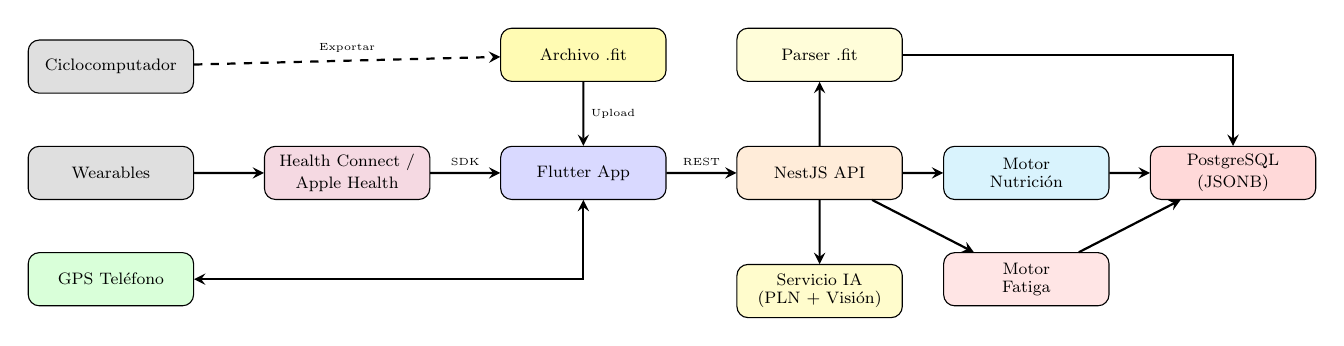
\begin{tikzpicture}[
    node distance=2cm,
    box/.style={draw, rectangle, rounded corners, minimum width=2.8cm, minimum height=0.9cm, fill=#1, text centered, font=\footnotesize},
    arrow/.style={->, thick, >=stealth},
    darrow/.style={<->, thick, >=stealth},
    dashed_arrow/.style={->, dashed, thick, >=stealth},
    scale=0.75, transform shape
]
    % External Layer - Left
    \node (ciclo) [box=gray!25] {Ciclocomputador};
    \node (wear) [box=gray!25, below of=ciclo, node distance=1.8cm] {Wearables};
    \node (gps) [box=green!15, below of=wear, node distance=1.8cm] {GPS Teléfono};

    % Broker Layer
    \node (hc) [box=purple!15, right of=wear, node distance=4cm] {\shortstack{Health Connect /\\Apple Health}};

    % App
    \node (app) [box=blue!15, right of=hc, node distance=4cm] {Flutter App};

    % File upload path
    \node (fit) [box=yellow!30, above of=app, node distance=2cm] {Archivo .fit};

    % Backend
    \node (api) [box=orange!15, right of=app, node distance=4cm] {NestJS API};

    % Backend modules
    \node (parser) [box=yellow!15, above of=api, node distance=2cm] {Parser .fit};
    \node (nutri) [box=cyan!15, right of=api, node distance=3.5cm] {\shortstack{Motor\\Nutrición}};
    \node (fatiga) [box=red!10, below of=nutri, node distance=1.8cm] {\shortstack{Motor\\Fatiga}};

    % AI
    \node (ai) [box=yellow!20, below of=api, node distance=2cm] {\shortstack{Servicio IA\\(PLN + Visión)}};

    % Database
    \node (db) [box=red!15, right of=nutri, node distance=3.5cm] {\shortstack{PostgreSQL\\(JSONB)}};

    % Arrows
    \draw[arrow] (wear) -- (hc);
    \draw[arrow] (hc) -- node[above, font=\tiny] {SDK} (app);
    \draw[darrow] (gps) -| (app);
    \draw[dashed_arrow] (ciclo) -- node[above, font=\tiny] {Exportar} (fit);
    \draw[arrow] (fit) -- node[right, font=\tiny] {Upload} (app);
    \draw[arrow] (app) -- node[above, font=\tiny] {REST} (api);
    \draw[arrow] (api) -- (parser);
    \draw[arrow] (api) -- (nutri);
    \draw[arrow] (api) -- (fatiga);
    \draw[arrow] (api) -- (ai);
    \draw[arrow] (nutri) -- (db);
    \draw[arrow] (fatiga) -- (db);
    \draw[arrow] (parser) -| (db);

\end{tikzpicture}
\captionof{figure}{Arquitectura técnica de la Solución (Alternativa 3).}
\label{fig:arquitectura_solucion}
\end{center}
\newpage
\subsubsection{Módulos Principales y Diagrama de Interacción}
La operación del ecosistema se divide en módulos funcionales que colaboran bidireccionalmente:

\textbf{1. Módulo de Ingesta de Telemetría (El Núcleo de Entrada)}\\
Se encarga de abstraer la fricción en la captura de datos del deportista mediante tres capas:
\begin{itemize}
    \item \textit{Capa Manual:} El usuario ingresa explícitamente sus rutinas (series, repeticiones, peso) o su RPE (Percepción Subjetiva del Esfuerzo).
    \item \textit{Capa de Brokers del SO:} La aplicación Flutter sincroniza asíncronamente en segundo plano con \textit{Health Connect} o \textit{Apple Health} para obtener métricas generales (pasos, calorías activas, frecuencia cardíaca basal).
    \item \textit{Capa Profunda (.fit):} Para deportistas que utilizan \textit{wearables} especializados (Garmin, Wahoo, Polar), la API recibe directamente archivos \texttt{.fit}. Un módulo especializado \textit{parser} en NestJS decodifica el archivo binario para extraer métricas precisas segundo a segundo (potencia en ciclismo, zonas cardíacas, altimetría).
\end{itemize}

\textbf{2. Motor de Fatiga y Planificación (La Lógica de Negocio Central)}\\
Este módulo cruza los datos fisiológicos provenientes del módulo de telemetría. Al final del día, o post-entrenamiento, el algoritmo evalúa la carga crónica (CTL) y aguda (ATL). Si el usuario registra una fatiga residual alta producto de una sesión de \textit{endurance} severa, pero tiene programada en su calendario una sesión de fuerza máxima al día siguiente, el motor emitirá una sugerencia activa (vía notificación *push*): recomendará disminuir el volumen de series o reducir la carga absoluta para evitar la interferencia concurrente y el sobreentrenamiento.

\textbf{3. Motor de Nutrición Asistida por IA}\\
Abandona los objetivos calóricos estáticos de la semana. Su interacción es totalmente dinámica y se acopla al motor de fatiga. Si se ejecutó un entrenamiento extenuante de alta duración, el módulo reajusta el \textit{Target} de carbohidratos diarios en la interfaz del usuario. Adicionalmente, el usuario interactúa enviando fotografías de sus comidas; NestJS remite la imagen junto a un \textit{prompt} sistémico a la API de Visión IA, obteniendo un cálculo aproximado de macronutrientes. Si el índice de confianza de la IA es bajo, exige validación del usuario, garantizando la integridad de los datos.

\textbf{4. Módulo Social y Comunidad}\\
Este módulo gestiona la gamificación y retención. Los usuarios pueden publicar sus entrenamientos y recetas. Lo que lo diferencia es su integración con el Motor de Nutrición: si un usuario ve la receta de "Panqueques Proteicos" de otro atleta, puede inyectarla en su propio diario. El backend escalará matemáticamente las porciones y los gramos de cada ingrediente para que cuadren matemáticamente con los requerimientos específicos del usuario que lo importa.

\vspace{0.5cm}
\begin{center}
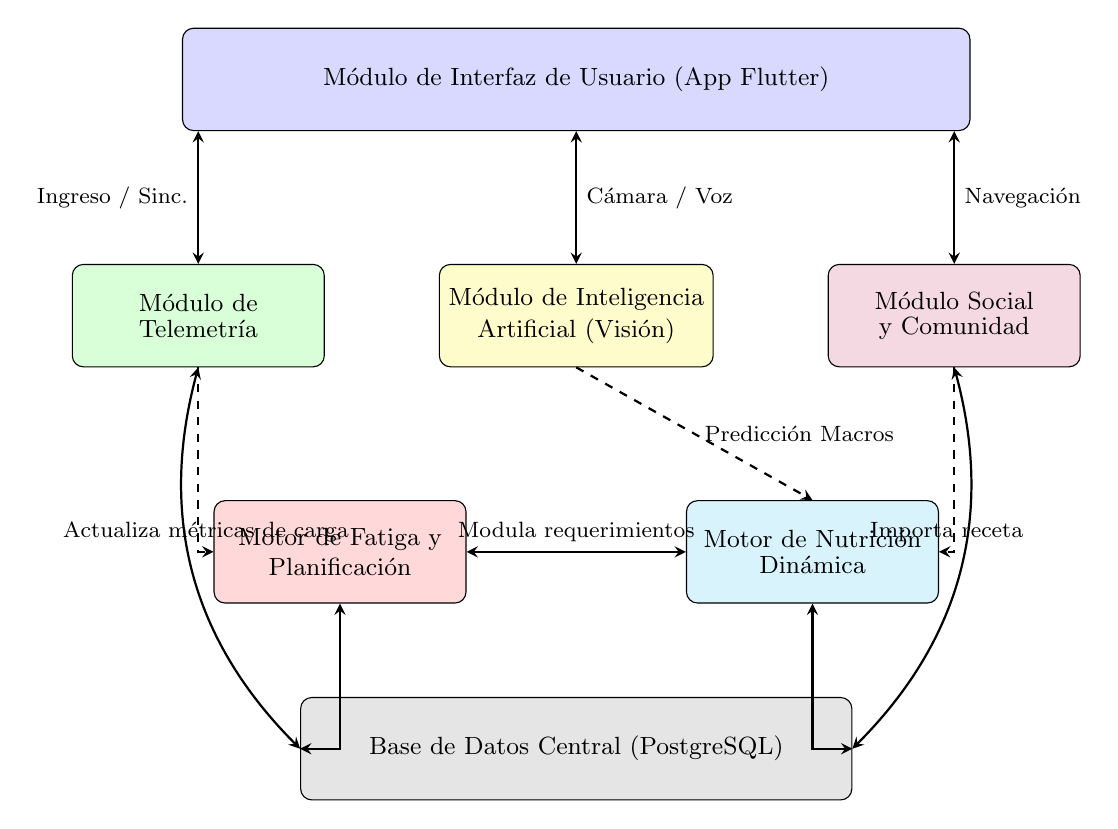
\begin{tikzpicture}[
    node distance=2.8cm,
    box/.style={draw, rectangle, rounded corners, minimum width=3.2cm, minimum height=1.3cm, fill=#1, text centered, font=\small},
    arrow/.style={->, thick, >=stealth},
    scale=1.0, transform shape
]
    % Central Hub
    \node (ui) [box=blue!15, minimum width=10cm] {Módulo de Interfaz de Usuario (App Flutter)};
    
    % Middle Layer
    \node (tel) [box=green!15, below of=ui, node distance=3cm, xshift=-4.8cm] {\shortstack{Módulo de\\Telemetría}};
    \node (ia) [box=yellow!20, below of=ui, node distance=3cm, xshift=0cm] {\shortstack{Módulo de Inteligencia\\Artificial (Visión)}};
    \node (soc) [box=purple!15, below of=ui, node distance=3cm, xshift=4.8cm] {\shortstack{Módulo Social\\y Comunidad}};
    
    % Core Layer
    \node (fat) [box=red!15, below of=tel, node distance=3cm, xshift=1.8cm] {\shortstack{Motor de Fatiga y\\Planificación}};
    \node (nut) [box=cyan!15, below of=soc, node distance=3cm, xshift=-1.8cm] {\shortstack{Motor de Nutrición\\Dinámica}};
    
    % DB Layer
    \node (db) [box=gray!20, below of=ia, node distance=5.5cm, minimum width=7cm] {Base de Datos Central (PostgreSQL)};

    % Arrows UI to Middle
    \draw[<->, thick, >=stealth] (ui.south -| tel.north) -- node[left, font=\footnotesize] {Ingreso / Sinc.} (tel.north);
    \draw[<->, thick, >=stealth] (ui.south) -- node[right, font=\footnotesize] {Cámara / Voz} (ia.north);
    \draw[<->, thick, >=stealth] (ui.south -| soc.north) -- node[right, font=\footnotesize] {Navegación} (soc.north);

    % Cross Interactions
    \draw[->, thick, >=stealth, dashed] (tel.south) |- node[above, font=\footnotesize, pos=0.75] {Actualiza métricas de carga} (fat.west);
    \draw[->, thick, >=stealth, dashed] (ia.south) -- node[right, font=\footnotesize] {Predicción Macros} (nut.north);
    
    % Fat and Nut Interaction
    \draw[<->, thick, >=stealth] (fat.east) -- node[above, font=\footnotesize] {Modula requerimientos} (nut.west);
    
    % Social to Nut/Fat
    \draw[->, thick, >=stealth, dashed] (soc.south) |- node[above, font=\footnotesize, pos=0.75] {Importa receta} (nut.east);

    % To DB
    \draw[<->, thick, >=stealth] (fat.south) |- (db.west);
    \draw[<->, thick, >=stealth] (nut.south) |- (db.east);
    \draw[<->, thick, >=stealth] (soc.south) to[bend left=30] (db.east);
    \draw[<->, thick, >=stealth] (tel.south) to[bend right=30] (db.west);

\end{tikzpicture}
\captionof{figure}{Diagrama de Interacción entre módulos funcionales.}
\label{fig:interaccion_modulos}
\end{center}
\newpage
\subsubsection{Modelo de Datos (Esquema Conceptual)}
Dada la naturaleza híbrida de los datos biológicos, el diseño de la base de datos PostgreSQL combinará esquemas relacionales estrictos con el almacenamiento de documentos. Las entidades principales serán:
\begin{itemize}
    \item \textbf{User (Usuario):} Almacena información biológica estática, metas (fuerza, resistencia, recomposición corporal), credenciales y \textit{tokens} de autorización hacia APIs de terceros.
    \item \textbf{DailyLog (Registro Diario):} Entidad transaccional vinculada a una fecha específica y a un usuario. Contiene los \textit{Targets} u objetivos calóricos del día generados de forma dinámica por el motor de fatiga.
    \item \textbf{Workout (Entrenamiento):} Relacionado al usuario, especifica si es una sesión cardiovascular o neuromuscular. En el caso de recibir telemetría compleja desde capas profundas, esta entidad contendrá un campo especializado \texttt{telemetry\_data} tipo \texttt{JSONB} que albergará vectores de potencia y pulsaciones sin desnormalizar la base de datos.
    \item \textbf{Meal (Comida):} Registro nutricional vinculado a un \textit{DailyLog}. Si la inserción provino del escáner de visión artificial, incluye un campo secundario llamado \texttt{ai\_confidence\_score} para trazabilidad.
\end{itemize}
\newpage
\subsubsection{Requerimientos de Infraestructura y Despliegue}
Para la puesta en marcha, la API de NestJS se orquestará utilizando contenedores \textbf{Docker}. Esto garantiza paridad entre el entorno de desarrollo y el de producción. La imagen compilada se desplegará en una plataforma de orquestación en la nube (como Google Cloud Run o AWS App Runner), la cual permite escalabilidad horizontal automática, absorbiendo picos de peticiones cuando los usuarios sincronicen sus dispositivos masivamente.
\\\\
La base de datos PostgreSQL se alojará en un servicio administrado (como Amazon RDS o Supabase) que garantice respaldos transaccionales automatizados (snapshots), recuperabilidad y encriptación de volúmenes, cumpliendo estrictamente con los mandatos de ciberseguridad delineados en la factibilidad operativa.
\newpage
\subsection{Beneficios del Proyecto}
La implementación de la plataforma tecnológica diseñada mediante la Alternativa 3 (Solución por Capas) plantea una serie de beneficios sustanciales, los cuales se pueden categorizar desde la perspectiva del usuario final (el atleta híbrido) y desde la perspectiva comercial del proyecto.

\textbf{Beneficios para el Usuario (Atleta Híbrido):}
\begin{itemize}
    \item \textbf{Centralización y Reducción de Fricción:} El atleta ya no requiere alternar entre tres aplicaciones distintas (registro de pesas, tracking GPS y contador de calorías). Todo su ecosistema deportivo converge en un único panel de control.
    \item \textbf{Prevención del Sobreentrenamiento (Fatiga Cruzada):} Al cruzar la métrica de carga aguda de resistencia con los entrenamientos de fuerza, el sistema protege la salud neuromuscular del usuario, alertando y reduciendo dinámicamente las cargas de gimnasio cuando el cuerpo no se encuentra recuperado, previniendo lesiones y estancamiento.
    \item \textbf{Nutrición de Precisión Adaptativa:} Al abandonar la ingesta calórica estática, el atleta asegura tener las reservas de glucógeno necesarias para los días de resistencia prolongada y las proteínas adecuadas para la reconstrucción muscular, maximizando la eficiencia biológica.
    \item \textbf{Interacción y Retención Comunitaria:} La capacidad de compartir rutinas y escalar recetas comunitarias automáticamente al perfil nutricional individual fomenta un sentido de pertenencia y motivación constante.
\end{itemize}
\newpage
\textbf{Beneficios Comerciales y Operativos:}
\begin{itemize}
    \item \textbf{Modelo SaaS Altamente Escalable:} Al basarse en infraestructura \textit{cloud} y procesamiento automatizado por IA, el costo marginal de integrar a un nuevo suscriptor a la plataforma es prácticamente nulo.
    \item \textbf{Alta Barrera de Salida (\textit{Lock-in} Tecnológico):} A medida que el usuario acumula telemetría histórica, el costo de cambiar a otra aplicación o volver al registro manual es inmenso, lo que asegura una altísima tasa de retención.
    \item \textbf{Monetización Directa:} El nicho de atletas híbridos posee una alta disposición a pagar por herramientas que mejoren su rendimiento, facilitando la captación de usuarios premium.
\end{itemize}
\newpage
\subsection{Análisis Costo - Beneficio}
El análisis de Costo-Beneficio contrasta los requerimientos financieros de capital necesarios para la puesta en marcha de la Solución por Capas frente a los retornos económicos y cualitativos proyectados en un horizonte temporal de 4 años.

\textbf{Estructura de Costos:}
\begin{itemize}
    \item \textbf{Inversión de Capital de Trabajo Inicial (CAPEX):} Como se determinó en la Factibilidad Económica, el desarrollo de la arquitectura completa (que integra IA, lectura de archivos \texttt{.fit}, \textit{backend} en NestJS y aplicación móvil en Flutter) exige una inversión inicial de \$19.220.000 CLP. Esta cifra engloba las horas de ingeniería de software.
    \item \textbf{Costos Operativos Anuales (OPEX):} El mantenimiento del ecosistema en la nube, consumo de APIs (IA) y licencias se estiman en \$2.883.000 CLP por año. A esto se le suma de manera indirecta el Costo de Adquisición de Clientes (CAC) y gastos de marketing.
\end{itemize}

\textbf{Estructura de Beneficios:}
\begin{itemize}
    \item \textbf{Ingresos Recurrentes Mensuales (MRR):} La plataforma monetizará a través de una suscripción premium fijada en \$7.990 CLP mensuales.
    \item \textbf{Punto de Equilibrio (Break-Even):} Los cálculos financieros demostraron que para absorber la alta inversión inicial y los costos operativos (logrando un VAN de 0 y una TIR del 15\%), el proyecto requiere fidelizar un promedio de \textbf{109 suscriptores anuales} constantes durante 4 años.
\end{itemize}

\textbf{Conclusión del Análisis:}\\
La relación Costo-Beneficio es ampliamente \textbf{favorable}. Si bien el proyecto requiere un esfuerzo de desarrollo significativo e incurre en los costos más altos dentro de las alternativas evaluadas, el retorno exigido de apenas 109 suscriptores es extremadamente bajo en relación con el tamaño del mercado. Los beneficios técnicos de centralizar la telemetría y la inteligencia artificial otorgan a la plataforma una ventaja competitiva abrumadora frente a soluciones aisladas, justificando económicamente el capital invertido y asegurando la sostenibilidad a largo plazo. Con esto, se da por finalizado el ciclo de análisis de factibilidad y definición arquitectónica.

\newpage
\section{Ingeniería de Requerimientos}
\subsection{Introducción del Capítulo}
En el presente capítulo se aborda la fase de Ingeniería de Requerimientos, un paso fundamental para traducir las necesidades de los atletas híbridos en especificaciones técnicas claras y medibles. A partir del análisis metodológico y de las alternativas evaluadas previamente, aquí se define el comportamiento esperado del sistema, la interacción de sus procesos principales y las restricciones bajo las cuales debe operar. En primer lugar, se presentará el Modelo de Negocios enfocado en los procesos operativos core de la plataforma, seguido por el modelo detallado de requerimientos funcionales y no funcionales, para finalmente establecer los Casos de Uso que guiarán la construcción de la arquitectura de software.

\subsection{Modelo de Negocios (Procesos Core)}
En el contexto de esta solución tecnológica, el modelo de negocios no hace referencia a un esquema financiero, sino que representa gráficamente el modelado de los macro-procesos operativos (\textit{Business Process Modeling}) que sustentan el valor de la aplicación. A continuación, se definen los flujos de trabajo principales mediante los cuales el sistema resuelve la problemática de fragmentación para el atleta híbrido.
\newpage
\subsubsection{Proceso de Sincronización y Cálculo de Fatiga Cruzada}
Este proceso describe cómo el ecosistema automatiza la captura de telemetría cardiovascular y modula la carga de entrenamiento concurrente. Su objetivo es identificar la fatiga residual antes de que el usuario incurra en sobreentrenamiento.

\begin{itemize}
    \item \textbf{Actores Involucrados:} Deportista Híbrido, Health Connect / Wearable, App Flutter (Cliente), API NestJS (Backend).
    \item \textbf{Descripción del Flujo:} El proceso inicia cuando el deportista finaliza su entrenamiento cardiovascular. El dispositivo físico (Wearable) sincroniza los datos (como archivos \texttt{.fit}) con el concentrador de salud del sistema operativo (Health Connect / Apple Health). La aplicación cliente detecta esta nueva telemetría y la transmite al servidor. En la nube, el Motor de Fatiga procesa las métricas de carga aguda. Si el sistema detecta que la fatiga residual es alta y existe un entrenamiento de fuerza programado para el día siguiente, se genera una alerta proactiva sugiriendo una reducción del volumen o intensidad. Finalmente, el nuevo estado fisiológico se almacena en la base de datos y se actualiza el panel de control del usuario.
\end{itemize}
\newpage
\textbf{Proceso de Sincronización y Cálculo de Fatiga Cruzada (BPMN)}
\begin{figure}[h!]
    \centering
    \includegraphics[width=1\textwidth]{bpmn_proceso1.png}
    \caption{BPMN: Sincronización de telemetría y cálculo de fatiga cruzada.}
    \label{fig:bpmn_fatiga}
\end{figure}
\newpage
\subsubsection{Proceso de Ajuste Nutricional Dinámico asistido por IA}
Este macro-proceso ilustra cómo la aplicación reduce la fricción del registro dietético y permite que la nutrición se adapte al gasto calórico del día, evitando el déficit de recuperación.

\begin{itemize}
    \item \textbf{Actores Involucrados:} Deportista Híbrido, App Flutter (Cliente), API NestJS (Backend), Servicio de IA (Visión).
    \item \textbf{Descripción del Flujo:} El usuario inicia el flujo capturando una fotografía de su alimento mediante la aplicación móvil. Esta imagen es enviada al servidor, el cual delega el análisis a un servicio de Inteligencia Artificial especializado en visión computacional. La IA estima los macronutrientes, porciones e ingredientes, devolviendo un índice de confianza. Si el índice de certeza es bajo, la aplicación exige que el usuario valide o corrija la lectura manualmente. Una vez confirmados los datos, el Motor de Nutrición descuenta el aporte calórico del objetivo dinámico diario y almacena la transacción en la base de datos, actualizando en tiempo real la barra de progreso nutricional en el dispositivo del atleta.
\end{itemize}
\newpage
\textbf{Proceso de Ajuste Nutricional Dinámico asistido por IA (BPMN)}
\begin{figure}[h!]
    \centering
    \includegraphics[width=1\textwidth]{bpmn_proceso2.png}
    \caption{BPMN: Registro de nutrición asistido por IA y ajuste dinámico.}
    \label{fig:bpmn_nutricion}
\end{figure}
\newpage
\subsubsection{Proceso de Importación y Escalado Dinámico de Recetas (Comunidad)}
Este proceso representa la gamificación y adherencia a través del módulo social, resolviendo el problema de adaptar preparaciones genéricas a los requerimientos altamente específicos de cada atleta.

\begin{itemize}
    \item \textbf{Actores Involucrados:} Deportista Híbrido, App Flutter (Cliente), API NestJS (Backend).
    \item \textbf{Descripción del Flujo:} El flujo comienza cuando el usuario navega por el feed de la comunidad y decide importar una receta compartida por otro atleta. Al solicitar la importación, la aplicación envía los datos de la receta y el estado actual del usuario al servidor. En el backend, el Motor Nutricional analiza la receta original y los macronutrientes que el usuario aún tiene pendientes por consumir en el día (los cuales ya fueron ajustados por el motor de fatiga). A través de un algoritmo de escalado, el sistema recalcula los gramos y porciones de cada ingrediente para que la comida encaje matemáticamente con el objetivo del usuario. Finalmente, la receta adaptada se guarda en el diario personal y se muestra en la interfaz para que el deportista proceda a cocinarla.
\end{itemize}
\newpage
\textbf{Proceso de Importación y Escalado Dinámico de Recetas (Comunidad) (BPMN)}
\begin{figure}[h!]
    \centering
    \includegraphics[width=1\textwidth]{bpmn_proceso3.png}
    \caption{BPMN: Importación y escalado dinámico de recetas comunitarias.}
    \label{fig:bpmn_recetas}
\end{figure}
\newpage
\subsubsection{Proceso de Registro de Fuerza mediante Lenguaje Natural (NLP)}
Este proceso busca reducir drásticamente la fricción al momento de registrar entrenamientos complejos de musculación, evitando los engorrosos formularios tradicionales manuales.

\begin{itemize}
    \item \textbf{Actores Involucrados:} Deportista Híbrido, App Flutter (Cliente), API NestJS (Backend), Servicio de IA (NLP).
    \item \textbf{Descripción del Flujo:} El usuario finaliza su sesión en el gimnasio y, en lugar de llenar celdas para cada ejercicio, dicta o escribe un párrafo en lenguaje natural (ej. "Hice 4 series de sentadillas con 100kg a 8 repeticiones"). La aplicación móvil envía este bloque de texto al servidor. El backend redirige el texto al servicio de Inteligencia Artificial (NLP), el cual procesa semánticamente la oración y estructura los datos en formato JSON, identificando el ejercicio, el peso, las repeticiones y la percepción subjetiva de esfuerzo (RPE) si se menciona. La API recibe los datos estructurados, valida las entidades contra la base de datos de ejercicios, guarda el registro de la sesión y, finalmente, dispara el cálculo de carga para actualizar el estado del atleta en la interfaz.
\end{itemize}
\newpage 
\textbf{Proceso de Registro de Fuerza mediante Lenguaje Natural (NLP) (BPMN)}
\begin{figure}[h!]
    \centering
    \includegraphics[width=1\textwidth]{bpmn_proceso4.png}
    \caption{BPMN: Registro de fuerza asistido por Procesamiento de Lenguaje Natural.}
    \label{fig:bpmn_nlp}
\end{figure}
\newpage
\subsection{Modelo de Requerimientos}
El Modelo de Requerimientos actúa como el puente formal entre las necesidades operativas del atleta híbrido y las especificaciones técnicas del software. A continuación, se presenta el diagrama de trazabilidad, el cual vincula explícitamente cada uno de los macro-procesos de negocio descritos en la sección anterior (Sincronización, IA Nutricional, Recetas y Registro NLP) con los requerimientos de sistema específicos que deben desarrollarse para hacerlos posibles. Este enfoque garantiza que ninguna funcionalidad del sistema se desarrolle aisladamente, sino que cada una contribuya directamente a la propuesta de valor del proyecto.

\begin{figure}[h!]
    \centering
    \includegraphics[width=0.9\textwidth]{diagrama_requerimientos.png}
    \caption{Diagrama de trazabilidad: Mapeo de Requerimientos a Procesos de Negocio.}
    \label{fig:diagrama_requerimientos}
\end{figure}
\newpage
\subsubsection{Requerimientos Funcionales}
Los requerimientos funcionales definen las capacidades operativas y de cálculo que el ecosistema tecnológico debe proveer. A continuación, se detallan en formato tabular los requerimientos clave extraídos del diagrama de trazabilidad.

\begin{table}[h!]
    \centering
    \renewcommand{\arraystretch}{1.3}
    \begin{tabular}{|p{3.5cm}|p{11.5cm}|}
        \hline
        \rowcolor[HTML]{EFEFEF} 
        \textbf{Identificador} & \textbf{RF-01} \\ \hline
        \textbf{Nombre} & Sincronización pasiva de telemetría cardiovascular \\ \hline
        \textbf{Descripción} & El sistema debe sincronizarse en segundo plano con las APIs de Health Connect (Android) y Apple HealthKit (iOS) para extraer datos biológicos básicos del usuario, incluyendo actividad diaria, frecuencia cardíaca basal y gasto calórico activo. \\ \hline
        \textbf{Prioridad} & Alta \\ \hline
        \textbf{Proceso Asociado} & Sincronización y Fatiga Cruzada \\ \hline
    \end{tabular}
\end{table}

\begin{table}[h!]
    \centering
    \renewcommand{\arraystretch}{1.3}
    \begin{tabular}{|p{3.5cm}|p{11.5cm}|}
        \hline
        \rowcolor[HTML]{EFEFEF} 
        \textbf{Identificador} & \textbf{RF-02} \\ \hline
        \textbf{Nombre} & Extracción y análisis de archivos de telemetría deportiva (.fit) \\ \hline
        \textbf{Descripción} & La API backend debe contar con un \textit{parser} capaz de decodificar archivos en formato \texttt{.fit} exportados desde ciclocomputadores y relojes Garmin/Polar, extrayendo los vectores de potencia, zonas cardíacas y estrés de entrenamiento (TSS). \\ \hline
        \textbf{Prioridad} & Alta \\ \hline
        \textbf{Proceso Asociado} & Sincronización y Fatiga Cruzada \\ \hline
    \end{tabular}
\end{table}

\begin{table}[h!]
    \centering
    \renewcommand{\arraystretch}{1.3}
    \begin{tabular}{|p{3.5cm}|p{11.5cm}|}
        \hline
        \rowcolor[HTML]{EFEFEF} 
        \textbf{Identificador} & \textbf{RF-03} \\ \hline
        \textbf{Nombre} & Motor de cálculo de fatiga cruzada y alertas proactivas \\ \hline
        \textbf{Descripción} & El sistema debe procesar la carga aguda (ATL) cardiovascular. Si la fatiga residual calculada supera el umbral de recuperación y el calendario del atleta indica una sesión de fuerza máxima al día siguiente, el sistema debe emitir una sugerencia para reducir el volumen de la sesión. \\ \hline
        \textbf{Prioridad} & Crítica \\ \hline
        \textbf{Proceso Asociado} & Sincronización y Fatiga Cruzada \\ \hline
    \end{tabular}
\end{table}
\newpage
\begin{table}[h!]
    \centering
    \renewcommand{\arraystretch}{1.3}
    \begin{tabular}{|p{3.5cm}|p{11.5cm}|}
        \hline
        \rowcolor[HTML]{EFEFEF} 
        \textbf{Identificador} & \textbf{RF-04} \\ \hline
        \textbf{Nombre} & Estimación nutricional mediante Visión Artificial \\ \hline
        \textbf{Descripción} & La aplicación móvil debe permitir capturar imágenes de platos de comida. El backend redirigirá la imagen a una API de Visión IA, la cual retornará un objeto JSON con los ingredientes detectados, porciones estimadas, macronutrientes e índice de confianza. \\ \hline
        \textbf{Prioridad} & Alta \\ \hline
        \textbf{Proceso Asociado} & Ajuste Nutricional con Inteligencia Artificial \\ \hline
    \end{tabular}
\end{table}

\begin{table}[h!]
    \centering
    \renewcommand{\arraystretch}{1.3}
    \begin{tabular}{|p{3.5cm}|p{11.5cm}|}
        \hline
        \rowcolor[HTML]{EFEFEF} 
        \textbf{Identificador} & \textbf{RF-05} \\ \hline
        \textbf{Nombre} & Algoritmo de escalado dinámico de recetas comunitarias \\ \hline
        \textbf{Descripción} & Al importar una receta desde el feed social, el sistema debe calcular la diferencia entre los requerimientos diarios totales del atleta y sus calorías ya consumidas, aplicando un multiplicador escalar a cada ingrediente de la receta original para que se ajuste exactamente al déficit actual. \\ \hline
        \textbf{Prioridad} & Media \\ \hline
        \textbf{Proceso Asociado} & Importación de Recetas (Social) \\ \hline
    \end{tabular}
\end{table}

\begin{table}[h!]
    \centering
    \renewcommand{\arraystretch}{1.3}
    \begin{tabular}{|p{3.5cm}|p{11.5cm}|}
        \hline
        \rowcolor[HTML]{EFEFEF} 
        \textbf{Identificador} & \textbf{RF-06} \\ \hline
        \textbf{Nombre} & Registro de fuerza estructurado mediante Lenguaje Natural (NLP) \\ \hline
        \textbf{Descripción} & El sistema debe proveer una interfaz de texto libre donde el usuario describa su sesión de pesas. El servidor debe enviar este texto a un modelo NLP y transformar la oración en una estructura de datos transaccional con ejercicio, series, repeticiones, peso y RPE. \\ \hline
        \textbf{Prioridad} & Alta \\ \hline
        \textbf{Proceso Asociado} & Registro de Fuerza (NLP) \\ \hline
    \end{tabular}
\end{table}

\begin{table}[h!]
    \centering
    \renewcommand{\arraystretch}{1.3}
    \begin{tabular}{|p{3.5cm}|p{11.5cm}|}
        \hline
        \rowcolor[HTML]{EFEFEF} 
        \textbf{Identificador} & \textbf{RF-07} \\ \hline
        \textbf{Nombre} & Registro manual de entrenamientos de fuerza \\ \hline
        \textbf{Descripción} & El sistema debe permitir a los usuarios buscar y seleccionar ejercicios desde un catálogo, e ingresar manualmente la cantidad de series, repeticiones, peso utilizado y esfuerzo percibido (RPE) para registrar una sesión estructurada. \\ \hline
        \textbf{Prioridad} & Alta \\ \hline
        \textbf{Proceso Asociado} & Registro y Seguimiento Core \\ \hline
    \end{tabular}
\end{table}

\begin{table}[h!]
    \centering
    \renewcommand{\arraystretch}{1.3}
    \begin{tabular}{|p{3.5cm}|p{11.5cm}|}
        \hline
        \rowcolor[HTML]{EFEFEF} 
        \textbf{Identificador} & \textbf{RF-08} \\ \hline
        \textbf{Nombre} & Registro manual de diario nutricional \\ \hline
        \textbf{Descripción} & El sistema debe proporcionar un buscador de alimentos por texto que permita a los usuarios ingresar gramos o porciones consumidas para añadirlas a su diario nutricional, descontando los valores de los macronutrientes objetivo diarios. \\ \hline
        \textbf{Prioridad} & Alta \\ \hline
        \textbf{Proceso Asociado} & Registro y Seguimiento Core \\ \hline
    \end{tabular}
\end{table}

\begin{table}[h!]
    \centering
    \renewcommand{\arraystretch}{1.3}
    \begin{tabular}{|p{3.5cm}|p{11.5cm}|}
        \hline
        \rowcolor[HTML]{EFEFEF} 
        \textbf{Identificador} & \textbf{RF-09} \\ \hline
        \textbf{Nombre} & Módulo de feed social y publicaciones \\ \hline
        \textbf{Descripción} & El sistema debe incluir un muro social interactivo donde los usuarios con perfil premium puedan publicar sus sesiones de entrenamiento finalizadas y recetas personalizadas para que sean visibles al resto de la comunidad. \\ \hline
        \textbf{Prioridad} & Media \\ \hline
        \textbf{Proceso Asociado} & Importación de Recetas (Social) \\ \hline
    \end{tabular}
\end{table}

\begin{table}[h!]
    \centering
    \renewcommand{\arraystretch}{1.3}
    \begin{tabular}{|p{3.5cm}|p{11.5cm}|}
        \hline
        \rowcolor[HTML]{EFEFEF} 
        \textbf{Identificador} & \textbf{RF-10} \\ \hline
        \textbf{Nombre} & Administración del catálogo de ejercicios \\ \hline
        \textbf{Descripción} & El sistema debe contar con un panel de administración (\textit{backoffice}) que permita al actor Administrador crear, leer, actualizar y eliminar (CRUD) registros de la base de datos maestra de ejercicios musculares. \\ \hline
        \textbf{Prioridad} & Alta \\ \hline
        \textbf{Proceso Asociado} & Administración de Plataforma \\ \hline
    \end{tabular}
\end{table}

\begin{table}[h!]
    \centering
    \renewcommand{\arraystretch}{1.3}
    \begin{tabular}{|p{3.5cm}|p{11.5cm}|}
        \hline
        \rowcolor[HTML]{EFEFEF} 
        \textbf{Identificador} & \textbf{RF-11} \\ \hline
        \textbf{Nombre} & Moderación de contenido comunitario \\ \hline
        \textbf{Descripción} & El sistema debe permitir al actor Administrador visualizar todo el contenido generado por los usuarios (UGC) en el feed social, y eliminar publicaciones o recetas que violen los lineamientos de la comunidad o presenten riesgos sanitarios. \\ \hline
        \textbf{Prioridad} & Media \\ \hline
        \textbf{Proceso Asociado} & Administración de Plataforma \\ \hline
    \end{tabular}
\end{table}
\newpage

\subsubsection{Características de los Usuarios del Sistema}
El sistema contempla tres perfiles de usuario con niveles de acceso diferenciados, diseñados para cubrir desde el deportista principiante hasta la administración técnica de la plataforma.

\begin{table}[h!]
    \centering
    \renewcommand{\arraystretch}{1.3}
    \begin{tabular}{|p{3cm}|p{4cm}|p{7.5cm}|}
        \hline
        \rowcolor[HTML]{EFEFEF}
        \textbf{Perfil} & \textbf{Nivel de Acceso} & \textbf{Descripción} \\ \hline
        Atleta Básico (Free) & Funcionalidades esenciales & Deportista aficionado que utiliza la plataforma para el registro manual de entrenamientos de fuerza y comidas. No requiere dispositivos externos. Su experiencia técnica es baja a media y su objetivo principal es llevar un seguimiento ordenado de su actividad. \\ \hline
        Atleta Híbrido (Premium) & Funcionalidades completas & Deportista que practica entrenamiento concurrente (fuerza + resistencia) y requiere el cruce de datos automatizado. Accede a la sincronización con \textit{wearables}, el escáner nutricional por IA, el registro por NLP, el motor de fatiga cruzada y el módulo social de recetas escalables. Posee experiencia media a alta con tecnología deportiva. \\ \hline
        Administrador & Panel de gestión interno & Perfil técnico responsable de la curación de la base de datos maestra de ejercicios, la moderación del contenido generado por la comunidad (recetas y publicaciones), y el monitoreo de métricas operativas del sistema (logs, rendimiento de la API, uso de cuotas de IA). \\ \hline
    \end{tabular}
    \caption{Perfiles de usuario del sistema.}
    \label{tab:perfiles_usuario}
\end{table}
\newpage
\subsubsection{Propósito del Sistema}
El propósito del sistema es centralizar la captura, el almacenamiento y el análisis cruzado de datos provenientes de tres dominios históricamente fragmentados: el entrenamiento de fuerza, la resistencia cardiovascular y la nutrición deportiva. A través de la integración de telemetría de \textit{wearables}, inteligencia artificial (visión computacional y procesamiento de lenguaje natural) y un motor algorítmico de fatiga concurrente, la plataforma busca:
\begin{enumerate}
    \item Automatizar el registro de sesiones deportivas y comidas, reduciendo la fricción operativa que genera el uso simultáneo de múltiples aplicaciones aisladas.
    \item Cuantificar objetivamente la fatiga cruzada entre disciplinas, permitiendo al atleta híbrido prevenir el sobreentrenamiento y el efecto de interferencia sin depender de estimaciones subjetivas.
    \item Adaptar dinámicamente los objetivos nutricionales diarios en función del desgaste fisiológico real, abandonando los modelos estáticos de calorías que no distinguen entre un día de descanso y un fondo largo en bicicleta.
    \item Fomentar la adherencia a largo plazo mediante un módulo social que permita compartir y escalar recetas comunitarias al perfil individual de cada usuario.
\end{enumerate}
\newpage
\subsubsection{Restricciones Generales}
Las siguientes restricciones condicionan el diseño, desarrollo y operación de la solución tecnológica:

\begin{itemize}
    \item \textbf{Dependencia de conectividad a Internet:} Los servicios de inteligencia artificial (visión y NLP) operan en la nube. El procesamiento de imágenes de alimentos y la interpretación de texto en lenguaje natural requieren una conexión activa a Internet. El registro manual de datos podrá funcionar con conectividad limitada mediante un sistema de cola local que sincronice al recuperar la conexión.
    \item \textbf{Restricción sanitaria y legal:} De acuerdo con el Código Sanitario (DFL N° 725) y la Ley N° 20.584, el sistema no emitirá diagnósticos médicos, prescripciones clínicas ni planes dietoterapéuticos. Todas las recomendaciones algorítmicas se presentarán como sugerencias de optimización deportiva, acompañadas de un \textit{disclaimer} legal permanente.
    \item \textbf{Protección de datos sensibles:} El tratamiento de biomarcadores (frecuencia cardíaca, peso corporal, ubicación GPS) debe cumplir íntegramente con la Ley N° 19.628 sobre Protección de la Vida Privada, implementando consentimiento explícito, derechos ARCO y cifrado obligatorio.
    \item \textbf{Dependencia de hardware de terceros:} La plataforma no desarrolla dispositivos propios. La captura de telemetría cardiovascular depende de la disponibilidad y compatibilidad de \textit{wearables} comerciales (Garmin, Polar, Apple Watch) y de los SDKs de Health Connect y Apple HealthKit.
    \item \textbf{Disciplinas deportivas acotadas:} El módulo de resistencia se limita exclusivamente a running y ciclismo. No se contempla soporte para natación, remo u otras disciplinas de resistencia.
    \item \textbf{Cuotas de API externas:} El consumo de servicios de IA generativa (OpenAI, Gemini) está sujeto a límites de uso (\textit{rate limits}) y costos por token. El diseño del backend debe implementar mecanismos de caché y control de gasto para evitar sobrecostos operativos.
\end{itemize}
\newpage
\subsubsection{Requisitos Específicos del Producto}
Los requisitos específicos detallan las capacidades particulares que cada módulo del producto debe ofrecer para satisfacer los requerimientos funcionales previamente definidos.

\begin{itemize}
    \item \textbf{Módulo de Fuerza:}
    \begin{itemize}
        \item El sistema debe mantener una base de datos maestra con al menos 200 ejercicios categorizados por grupo muscular, patrón de movimiento y equipamiento requerido.
        \item El usuario debe poder crear ejercicios personalizados que se almacenen en su perfil individual.
        \item Cada serie registrada debe contener como mínimo: ejercicio, peso (kg), repeticiones y, opcionalmente, RPE (escala 1--10).
        \item El registro por NLP debe soportar la entrada de múltiples ejercicios en un solo bloque de texto.
    \end{itemize}
    \item \textbf{Módulo de Resistencia (Cardio):}
    \begin{itemize}
        \item El sistema debe sincronizar automáticamente las sesiones de running y ciclismo registradas en Health Connect o Apple HealthKit.
        \item El \textit{parser} de archivos \texttt{.fit} debe extraer, como mínimo: duración, distancia, frecuencia cardíaca promedio y máxima, potencia promedio (si aplica), cadencia y Training Stress Score (TSS).
        \item La telemetría segundo a segundo debe almacenarse en campos \texttt{JSONB} dentro de la entidad \texttt{Workout}.
    \end{itemize}
    \item \textbf{Módulo de Nutrición:}
    \begin{itemize}
        \item El escáner de visión artificial debe retornar una estimación de calorías totales, proteínas (g), carbohidratos (g) y grasas (g) junto con un índice de confianza (0--100\%).
        \item Si el índice de confianza es inferior al 70\%, el sistema debe solicitar validación manual obligatoria al usuario antes de registrar la comida.
        \item El usuario debe poder guardar comidas frecuentes como plantillas reutilizables.
    \end{itemize}
    \item \textbf{Motor de Fatiga y Cruce de Datos:}
    \begin{itemize}
        \item El motor debe calcular diariamente la carga aguda (ATL) y crónica (CTL) del atleta, utilizando un modelo de media móvil exponencial ponderada.
        \item Las alertas de fatiga cruzada deben generarse cuando el ratio ATL/CTL supere un umbral configurable y exista una sesión de la disciplina opuesta programada en las próximas 24 horas.
    \end{itemize}
    \item \textbf{Módulo Social:}
    \begin{itemize}
        \item Los usuarios premium deben poder publicar entrenamientos y recetas en un feed comunitario.
        \item El algoritmo de escalado debe recalcular los gramos de cada ingrediente proporcionalmente, manteniendo las proporciones de la receta original y ajustando el total calórico al déficit o superávit restante del usuario importador.
    \end{itemize}
\end{itemize}
\newpage
\subsubsection{Requisitos No Funcionales}
Los requisitos no funcionales establecen los atributos de calidad bajo los cuales el sistema debe operar para garantizar una experiencia confiable, segura y escalable.

\begin{table}[h!]
    \centering
    \renewcommand{\arraystretch}{1.3}
    \begin{tabular}{|p{3.5cm}|p{11.5cm}|}
        \hline
        \rowcolor[HTML]{EFEFEF}
        \textbf{Identificador} & \textbf{RNF-01} \\ \hline
        \textbf{Categoría} & Rendimiento \\ \hline
        \textbf{Descripción} & El servicio de estimación nutricional por visión artificial debe retornar los resultados al cliente en un tiempo máximo de 5 segundos bajo condiciones normales de red. \\ \hline
    \end{tabular}
\end{table}

\begin{table}[h!]
    \centering
    \renewcommand{\arraystretch}{1.3}
    \begin{tabular}{|p{3.5cm}|p{11.5cm}|}
        \hline
        \rowcolor[HTML]{EFEFEF}
        \textbf{Identificador} & \textbf{RNF-02} \\ \hline
        \textbf{Categoría} & Rendimiento \\ \hline
        \textbf{Descripción} & El \textit{parser} de archivos \texttt{.fit} debe procesar archivos de hasta 10 MB (equivalente a aproximadamente 4 horas de telemetría continua) en menos de 3 segundos en el servidor. \\ \hline
    \end{tabular}
\end{table}

\begin{table}[h!]
    \centering
    \renewcommand{\arraystretch}{1.3}
    \begin{tabular}{|p{3.5cm}|p{11.5cm}|}
        \hline
        \rowcolor[HTML]{EFEFEF}
        \textbf{Identificador} & \textbf{RNF-03} \\ \hline
        \textbf{Categoría} & Seguridad \\ \hline
        \textbf{Descripción} & Toda comunicación entre el cliente móvil y la API NestJS debe realizarse mediante protocolo HTTPS con TLS 1.3. Los \textit{tokens} de autorización hacia \textit{brokers} de salud y las credenciales sensibles deben almacenarse cifrados en reposo (AES-256) en la base de datos PostgreSQL. \\ \hline
    \end{tabular}
\end{table}

\begin{table}[h!]
    \centering
    \renewcommand{\arraystretch}{1.3}
    \begin{tabular}{|p{3.5cm}|p{11.5cm}|}
        \hline
        \rowcolor[HTML]{EFEFEF}
        \textbf{Identificador} & \textbf{RNF-04} \\ \hline
        \textbf{Categoría} & Seguridad y Privacidad \\ \hline
        \textbf{Descripción} & El sistema debe implementar un flujo de consentimiento explícito durante el \textit{onboarding} antes de acceder a cualquier dato biométrico. Debe proveer mecanismos de derechos ARCO (Acceso, Rectificación, Cancelación y Oposición) y un botón de eliminación absoluta de cuenta con borrado en cascada, en cumplimiento de la Ley N° 19.628. \\ \hline
    \end{tabular}
\end{table}
\newpage
\begin{table}[h!]
    \centering
    \renewcommand{\arraystretch}{1.3}
    \begin{tabular}{|p{3.5cm}|p{11.5cm}|}
        \hline
        \rowcolor[HTML]{EFEFEF}
        \textbf{Identificador} & \textbf{RNF-05} \\ \hline
        \textbf{Categoría} & Escalabilidad \\ \hline
        \textbf{Descripción} & El backend NestJS debe desplegarse en contenedores Docker sobre una plataforma de orquestación en la nube (Google Cloud Run o AWS App Runner) que permita escalamiento horizontal automático para absorber picos de sincronización simultánea de \textit{wearables}. \\ \hline
    \end{tabular}
\end{table}

\begin{table}[h!]
    \centering
    \renewcommand{\arraystretch}{1.3}
    \begin{tabular}{|p{3.5cm}|p{11.5cm}|}
        \hline
        \rowcolor[HTML]{EFEFEF}
        \textbf{Identificador} & \textbf{RNF-06} \\ \hline
        \textbf{Categoría} & Disponibilidad \\ \hline
        \textbf{Descripción} & La base de datos PostgreSQL debe alojarse en un servicio administrado con respaldos transaccionales automatizados (\textit{snapshots}) diarios y capacidad de recuperación ante desastres (RPO $<$ 24 horas). \\ \hline
    \end{tabular}
\end{table}

\begin{table}[h!]
    \centering
    \renewcommand{\arraystretch}{1.3}
    \begin{tabular}{|p{3.5cm}|p{11.5cm}|}
        \hline
        \rowcolor[HTML]{EFEFEF}
        \textbf{Identificador} & \textbf{RNF-07} \\ \hline
        \textbf{Categoría} & Usabilidad \\ \hline
        \textbf{Descripción} & La aplicación móvil debe seguir las directrices de Material Design 3 (Android) y las guías de interfaz humana de Apple (iOS), garantizando una experiencia consistente y nativa en ambas plataformas mediante Flutter. \\ \hline
    \end{tabular}
\end{table}

\begin{table}[h!]
    \centering
    \renewcommand{\arraystretch}{1.3}
    \begin{tabular}{|p{3.5cm}|p{11.5cm}|}
        \hline
        \rowcolor[HTML]{EFEFEF}
        \textbf{Identificador} & \textbf{RNF-08} \\ \hline
        \textbf{Categoría} & Mantenibilidad \\ \hline
        \textbf{Descripción} & El código fuente del backend debe estructurarse en módulos desacoplados siguiendo el patrón de inyección de dependencias nativo de NestJS, facilitando la incorporación futura de nuevas disciplinas deportivas o servicios de IA sin modificar los módulos existentes. \\ \hline
    \end{tabular}
\end{table}
\newpage
\subsubsection{Requisitos de las Interfaces}
Los requisitos de interfaz especifican cómo el sistema se comunica con los usuarios, con otros sistemas de software y con los dispositivos de hardware externos.
\\\\
\textbf{Interfaces de Usuario (UI):}
\begin{itemize}
    \item La interfaz principal será una aplicación móvil multiplataforma desarrollada en Flutter (Dart), compilada de forma nativa para iOS y Android.
    \item El diseño visual debe seguir los principios de Material Design 3, priorizando la legibilidad de datos numéricos (macronutrientes, series, pesos) y la navegación rápida entre los módulos de fuerza, cardio y nutrición.
    \item La interfaz debe soportar el modo oscuro y adaptarse a diferentes tamaños de pantalla (desde 4.7 hasta 6.7 pulgadas).
    \item Los formularios de registro deben incluir validaciones en tiempo real y retroalimentación visual inmediata (colores de barra de progreso para macronutrientes cumplidos vs. pendientes).
\end{itemize}

\textbf{Interfaces de Software:}
\begin{itemize}
    \item \textbf{Health Connect (Android) y Apple HealthKit (iOS):} Integración mediante los SDKs nativos oficiales para lectura de actividades físicas, frecuencia cardíaca, pasos y gasto calórico. La escritura se limita a exportar los datos nutricionales registrados en la plataforma.
    \item \textbf{APIs de IA Generativa:} Comunicación vía API REST (HTTPS) con servicios como Gemini 1.5 Pro u OpenAI para el procesamiento de imágenes de alimentos (visión) y la interpretación de rutinas en lenguaje natural (NLP). Las solicitudes incluyen un \textit{prompt} sistémico predefinido para estructurar las respuestas en formato JSON.
    \item \textbf{Almacenamiento en la nube:} Integración con un servicio de almacenamiento de objetos (Amazon S3 o equivalente) para persistir las fotografías de comidas y los archivos \texttt{.fit} cargados por los usuarios.
\end{itemize}

\textbf{Interfaces de Comunicación:}
\begin{itemize}
    \item Toda la comunicación entre el cliente Flutter y el backend NestJS se realizará mediante una API RESTful sobre protocolo HTTPS, utilizando JSON como formato de intercambio de datos.
    \item El sistema de autenticación se implementará mediante tokens JWT (\textit{JSON Web Tokens}) con un esquema de \textit{access token} de corta duración y \textit{refresh token} de larga duración para mantener sesiones seguras sin solicitar credenciales repetidamente.
    \item Las notificaciones \textit{push} (alertas de fatiga cruzada, recordatorios nutricionales) se enviarán a través de Firebase Cloud Messaging (FCM), compatible con ambas plataformas móviles.
\end{itemize}

\textbf{Interfaces de Hardware:}
\begin{itemize}
    \item \textbf{Cámara del dispositivo:} Acceso al módulo de cámara del teléfono para capturar fotografías de alimentos destinadas al escáner nutricional por IA.
    \item \textbf{GPS del dispositivo:} Acceso al sensor de ubicación para el registro opcional de rutas de running o ciclismo cuando el usuario no disponga de un \textit{wearable} externo.
    \item \textbf{Wearables y ciclocomputadores:} Comunicación indirecta a través de los concentradores del sistema operativo (Health Connect / HealthKit). No se establece conexión Bluetooth directa entre la aplicación y los dispositivos; toda la telemetría fluye mediante los \textit{brokers} nativos del SO o la carga manual de archivos \texttt{.fit}.
\end{itemize}
\newpage
\subsection{Casos de Uso}
\subsubsection{Actores}
Los actores representan las entidades externas que interactúan con el sistema. Se clasifican en actores primarios (quienes inician las acciones) y actores secundarios (sistemas externos que participan en los flujos).

\begin{table}[h!]
    \centering
    \renewcommand{\arraystretch}{1.3}
    \begin{tabular}{|p{1cm}|p{3.5cm}|p{2cm}|p{8cm}|}
        \hline
        \rowcolor[HTML]{EFEFEF}
        \textbf{ID} & \textbf{Actor} & \textbf{Tipo} & \textbf{Descripción} \\ \hline
        A-01 & Atleta Básico & Primario & Usuario registrado en el plan gratuito. Puede registrar entrenamientos de fuerza manualmente y llevar un diario nutricional básico. \\ \hline
        A-02 & Atleta Híbrido & Primario & Usuario suscrito al plan premium. Hereda todas las capacidades del Atleta Básico y accede a la sincronización de telemetría, el escáner nutricional por IA, el registro por NLP, el motor de fatiga cruzada y el módulo social. \\ \hline
        A-03 & Administrador & Primario & Operador técnico que gestiona la base de datos de ejercicios, modera el contenido de la comunidad y monitorea las métricas operativas del sistema. \\ \hline
        A-04 & Health Connect / Apple HealthKit & Secundario & Concentrador de datos del sistema operativo móvil. Provee telemetría cardiovascular, pasos y frecuencia cardíaca de los \textit{wearables} del usuario de forma pasiva. \\ \hline
        A-05 & Servicio de IA & Secundario & API externa de inteligencia artificial (Gemini / OpenAI) que procesa imágenes de alimentos (visión) y bloques de texto de rutinas (NLP), retornando datos estructurados. \\ \hline
        A-06 & Firebase (FCM) & Secundario & Servicio de mensajería en la nube que entrega las notificaciones \textit{push} (alertas de fatiga, recordatorios nutricionales) a los dispositivos de los usuarios. \\ \hline
    \end{tabular}
    \caption{Actores del sistema.}
    \label{tab:actores}
\end{table}
\newpage
\subsubsection{Diagrama de Casos de Uso}
A continuación, se presentan los diagramas de casos de uso del sistema, organizados en tres vistas complementarias: un diagrama general que muestra la interacción global de los actores con la plataforma, y dos diagramas detallados que profundizan en los subsistemas de Entrenamiento y de Nutrición/Social respectivamente.

% TODO: Insertar diagrama general de casos de uso
\begin{figure}[h!]
    \centering
    \includegraphics[width=0.85\textwidth]{cu_general.png}
    \caption{Diagrama general de Casos de Uso del sistema.}
    \label{fig:cu_general}
\end{figure}


% TODO: Insertar diagrama de casos de uso - Subsistema Entrenamiento
\begin{figure}[h!]
    \centering
    \includegraphics[width=0.85\textwidth]{cu_entrenamiento.png}
    \caption{Diagrama de Casos de Uso: Subsistema de Entrenamiento (Fuerza y Resistencia).}
    \label{fig:cu_entrenamiento}
\end{figure}

\newpage

% TODO: Insertar diagrama de casos de uso - Subsistema Nutrición y Social
\begin{figure}[h!]
    \centering
    \includegraphics[width=0.85\textwidth]{cu_nutricion.png}
    \caption{Diagrama de Casos de Uso: Subsistema de Nutrición y Comunidad.}
    \label{fig:cu_nutricion}
\end{figure}
\newpage
\subsubsection{Descripción de Alto Nivel de Casos de Uso}
A continuación, se describen los casos de uso identificados en los diagramas anteriores, indicando su relación con los requerimientos funcionales definidos.

\begin{table}[h!]
    \centering
    \renewcommand{\arraystretch}{1.3}
    \begin{tabular}{|p{3.5cm}|p{11.5cm}|}
        \hline
        \rowcolor[HTML]{EFEFEF}
        \textbf{Identificador} & \textbf{CU-01} \\ \hline
        \textbf{Nombre} & Registrar entrenamiento de fuerza (manual) \\ \hline
        \textbf{Actor Principal} & Atleta Básico / Atleta Híbrido \\ \hline
        \textbf{Descripción} & El usuario selecciona ejercicios desde la base de datos maestra o sus ejercicios personalizados, e ingresa manualmente las series, repeticiones, peso y RPE de su sesión. El sistema almacena la sesión y actualiza la carga de fuerza acumulada. \\ \hline
        \textbf{RF Asociados} & RF-07 \\ \hline
    \end{tabular}
\end{table}

\begin{table}[h!]
    \centering
    \renewcommand{\arraystretch}{1.3}
    \begin{tabular}{|p{3.5cm}|p{11.5cm}|}
        \hline
        \rowcolor[HTML]{EFEFEF}
        \textbf{Identificador} & \textbf{CU-02} \\ \hline
        \textbf{Nombre} & Registrar entrenamiento de fuerza por NLP \\ \hline
        \textbf{Actor Principal} & Atleta Híbrido \\ \hline
        \textbf{Actores Secundarios} & Servicio de IA (NLP) \\ \hline
        \textbf{Descripción} & El usuario dicta o escribe un párrafo describiendo su sesión de pesas en lenguaje natural. El sistema envía el texto al servicio de IA, recibe la estructura JSON con los ejercicios identificados y permite al usuario confirmar o corregir antes de guardar. \\ \hline
        \textbf{RF Asociados} & RF-06 \\ \hline
    \end{tabular}
\end{table}

\begin{table}[h!]
    \centering
    \renewcommand{\arraystretch}{1.3}
    \begin{tabular}{|p{3.5cm}|p{11.5cm}|}
        \hline
        \rowcolor[HTML]{EFEFEF}
        \textbf{Identificador} & \textbf{CU-03} \\ \hline
        \textbf{Nombre} & Sincronizar telemetría cardiovascular \\ \hline
        \textbf{Actor Principal} & Atleta Híbrido \\ \hline
        \textbf{Actores Secundarios} & Health Connect / Apple HealthKit \\ \hline
        \textbf{Descripción} & La aplicación detecta automáticamente nuevas sesiones de running o ciclismo registradas en el concentrador de salud del sistema operativo. Los datos se extraen, se envían al backend y se almacenan como un entrenamiento cardiovascular con sus métricas asociadas. \\ \hline
        \textbf{RF Asociados} & RF-01 \\ \hline
    \end{tabular}
\end{table}
\newpage
\begin{table}[h!]
    \centering
    \renewcommand{\arraystretch}{1.3}
    \begin{tabular}{|p{3.5cm}|p{11.5cm}|}
        \hline
        \rowcolor[HTML]{EFEFEF}
        \textbf{Identificador} & \textbf{CU-04} \\ \hline
        \textbf{Nombre} & Cargar y procesar archivo .fit \\ \hline
        \textbf{Actor Principal} & Atleta Híbrido \\ \hline
        \textbf{Descripción} & El usuario exporta un archivo \texttt{.fit} desde su ciclocomputador o reloj deportivo y lo sube a través de la aplicación. El backend decodifica el archivo binario, extrae la telemetría segundo a segundo (potencia, cadencia, zonas cardíacas, TSS) y la almacena en un campo JSONB dentro de la entidad Workout. \\ \hline
        \textbf{RF Asociados} & RF-02 \\ \hline
    \end{tabular}
\end{table}

\begin{table}[h!]
    \centering
    \renewcommand{\arraystretch}{1.3}
    \begin{tabular}{|p{3.5cm}|p{11.5cm}|}
        \hline
        \rowcolor[HTML]{EFEFEF}
        \textbf{Identificador} & \textbf{CU-05} \\ \hline
        \textbf{Nombre} & Consultar análisis de fatiga cruzada \\ \hline
        \textbf{Actor Principal} & Atleta Híbrido \\ \hline
        \textbf{Actores Secundarios} & Firebase (FCM) \\ \hline
        \textbf{Descripción} & Tras cada entrenamiento registrado o sincronizado, el motor de fatiga recalcula la carga aguda (ATL) y crónica (CTL). Si el ratio supera el umbral configurable y existe una sesión de la disciplina opuesta en las próximas 24 horas, el sistema genera una alerta \textit{push} y muestra la recomendación de modulación en el dashboard. \\ \hline
        \textbf{RF Asociados} & RF-03 \\ \hline
    \end{tabular}
\end{table}

\begin{table}[h!]
    \centering
    \renewcommand{\arraystretch}{1.3}
    \begin{tabular}{|p{3.5cm}|p{11.5cm}|}
        \hline
        \rowcolor[HTML]{EFEFEF}
        \textbf{Identificador} & \textbf{CU-06} \\ \hline
        \textbf{Nombre} & Registrar comida manual \\ \hline
        \textbf{Actor Principal} & Atleta Básico / Atleta Híbrido \\ \hline
        \textbf{Descripción} & El usuario busca alimentos en la base de datos nutricional, selecciona las porciones consumidas y registra la comida en su diario del día. El sistema actualiza el balance de macronutrientes y la barra de progreso calórico. \\ \hline
        \textbf{RF Asociados} & RF-08 \\ \hline
    \end{tabular}
\end{table}
\newpage
\begin{table}[h!]
    \centering
    \renewcommand{\arraystretch}{1.3}
    \begin{tabular}{|p{3.5cm}|p{11.5cm}|}
        \hline
        \rowcolor[HTML]{EFEFEF}
        \textbf{Identificador} & \textbf{CU-07} \\ \hline
        \textbf{Nombre} & Registrar comida por fotografía (IA) \\ \hline
        \textbf{Actor Principal} & Atleta Híbrido \\ \hline
        \textbf{Actores Secundarios} & Servicio de IA (Visión) \\ \hline
        \textbf{Descripción} & El usuario captura una fotografía de su plato. El sistema la envía al servicio de visión IA, el cual retorna una estimación de ingredientes, porciones y macronutrientes con un índice de confianza. Si la confianza es inferior al 70\%, se solicita validación manual antes de confirmar el registro. \\ \hline
        \textbf{RF Asociados} & RF-04 \\ \hline
    \end{tabular}
\end{table}

\begin{table}[h!]
    \centering
    \renewcommand{\arraystretch}{1.3}
    \begin{tabular}{|p{3.5cm}|p{11.5cm}|}
        \hline
        \rowcolor[HTML]{EFEFEF}
        \textbf{Identificador} & \textbf{CU-08} \\ \hline
        \textbf{Nombre} & Importar y escalar receta comunitaria \\ \hline
        \textbf{Actor Principal} & Atleta Híbrido \\ \hline
        \textbf{Descripción} & El usuario selecciona una receta publicada por otro atleta en el feed social y solicita importarla a su diario. El motor nutricional calcula los macronutrientes pendientes del día y aplica un multiplicador escalar a los ingredientes de la receta original, ajustando las porciones al objetivo individual del usuario. \\ \hline
        \textbf{RF Asociados} & RF-05 \\ \hline
    \end{tabular}
\end{table}

\begin{table}[h!]
    \centering
    \renewcommand{\arraystretch}{1.3}
    \begin{tabular}{|p{3.5cm}|p{11.5cm}|}
        \hline
        \rowcolor[HTML]{EFEFEF}
        \textbf{Identificador} & \textbf{CU-09} \\ \hline
        \textbf{Nombre} & Publicar entrenamiento o receta en la comunidad \\ \hline
        \textbf{Actor Principal} & Atleta Híbrido \\ \hline
        \textbf{Descripción} & El usuario selecciona un entrenamiento completado o una receta guardada y la publica en el feed comunitario para que otros atletas puedan visualizarla, comentarla o importarla a su propio diario. \\ \hline
        \textbf{RF Asociados} & RF-09 \\ \hline
    \end{tabular}
\end{table}

\begin{table}[h!]
    \centering
    \renewcommand{\arraystretch}{1.3}
    \begin{tabular}{|p{3.5cm}|p{11.5cm}|}
        \hline
        \rowcolor[HTML]{EFEFEF}
        \textbf{Identificador} & \textbf{CU-10} \\ \hline
        \textbf{Nombre} & Gestionar base de datos de ejercicios \\ \hline
        \textbf{Actor Principal} & Administrador \\ \hline
        \textbf{Descripción} & El administrador puede crear, editar y eliminar ejercicios de la base de datos maestra del sistema, categorizándolos por grupo muscular, patrón de movimiento y equipamiento requerido. \\ \hline
        \textbf{RF Asociados} & RF-10 \\ \hline
    \end{tabular}
\end{table}
\newpage
\begin{table}[ht!]
    \centering
    \renewcommand{\arraystretch}{1.3}
    \begin{tabular}{|p{3.5cm}|p{11.5cm}|}
        \hline
        \rowcolor[HTML]{EFEFEF}
        \textbf{Identificador} & \textbf{CU-11} \\ \hline
        \textbf{Nombre} & Moderar contenido de la comunidad \\ \hline
        \textbf{Actor Principal} & Administrador \\ \hline
        \textbf{Descripción} & El administrador revisa y puede eliminar o suspender publicaciones, recetas o comentarios del feed comunitario que infrinjan las normas de uso de la plataforma o contengan información nutricional potencialmente dañina. \\ \hline
        \textbf{RF Asociados} & RF-11 \\ \hline
    \end{tabular}
\end{table}
\subsection{Comentarios Generales del Capítulo}
En este capítulo se ha consolidado el puente entre la visión de negocio y la implementación técnica de la plataforma. Iniciando con un Modelo de Negocios basado en cuatro macro-procesos fundamentales (sincronización biométrica, ajuste nutricional asistido por IA, registro mediante procesamiento de lenguaje natural y escalamiento social de recetas), se logró establecer una propuesta de valor clara y medible. Posteriormente, la trazabilidad de los requerimientos garantizó que cada especificación funcional y no funcional del software nazca directamente de una necesidad operativa comprobada, mitigando el riesgo de desarrollar funcionalidades superfluas. 

Finalmente, la especificación de los Casos de Uso, apoyada por sus respectivos diagramas e identificación de actores primarios y secundarios, delimitó con exactitud la frontera del sistema. Con este sólido marco de requerimientos finalizado, alineado a las restricciones normativas chilenas y a las dependencias de hardware de terceros, el proyecto cuenta con las bases necesarias para transicionar hacia la fase de Ingeniería de Diseño, donde se definirá la arquitectura de software detallada, el modelo de datos relacional y las interfaces de usuario.\newpage
\newpage
\section{Ingeniería de Diseño}
\subsection{Introducción del Capítulo}
El presente capítulo detalla la Ingeniería de Diseño de la solución tecnológica. Tomando como base los requerimientos funcionales y las restricciones operativas definidas en el capítulo anterior, aquí se materializa la arquitectura del software, la estructuración de la base de datos, el diseño de las interfaces de usuario y el modelo de interacciones. El objetivo de este diseño es garantizar que la plataforma sea escalable, segura y capaz de procesar la telemetría concurrente y los modelos de inteligencia artificial de forma eficiente.

\subsection{Diagrama de Sistema de Alto Nivel}
El diagrama de sistema de alto nivel presenta una vista macroscópica de la arquitectura de la plataforma, modelada bajo un enfoque cliente-servidor basado en API RESTful. La arquitectura se divide en tres grandes capas: la capa de presentación (cliente móvil), la capa de procesamiento central (backend en la nube) y la capa de servicios externos.

% TODO: Insertar diagrama de arquitectura de alto nivel
\begin{figure}[h!]
    \centering
    \includegraphics[width=1\textwidth]{diagrama_arquitectura.png}
    \caption{Arquitectura de Alto Nivel del Sistema.}
    \label{fig:arquitectura_alto_nivel}
\end{figure}
\newpage
Como se observa en el diagrama, el flujo de información comienza en el \textbf{Dispositivo Móvil}, donde la aplicación construida en \textbf{Flutter} gestiona la interacción directa con el usuario y actúa como receptor pasivo de la telemetría proveniente de los concentradores nativos (\textit{Health Connect} o \textit{Apple HealthKit}). 

Toda la carga de procesamiento biomédico y lógica de negocio se delega a la \textbf{Infraestructura Cloud}. Allí, una API desarrollada en \textbf{NestJS} actúa como orquestador central (BFF - \textit{Backend for Frontend}). Esta API es la única entidad con acceso directo a la base de datos \textbf{PostgreSQL}, asegurando la integridad de los datos mediante consultas tipadas. 

Finalmente, para mantener el backend ligero y enfocado en la lógica del negocio deportivo, el sistema se apoya en \textbf{Servicios Externos} altamente especializados: \textit{Amazon S3} para el almacenamiento de archivos binarios (fotos y telemetría \texttt{.fit}), \textit{Firebase Cloud Messaging (FCM)} para el envío de alertas de fatiga asíncronas, y las APIs de \textit{Inteligencia Artificial (Gemini/OpenAI)} para delegar la carga computacional de los algoritmos de visión y NLP.
\newpage
\subsection{Diseño Funcional}
A continuación se presentan los cursos normales y alternos de los eventos para cada uno de los Casos de Uso descritos previamente en la fase de requerimientos.

\subsubsection{CU-01. Registrar entrenamiento de fuerza (manual)}

\textbf{Diagrama de Actividades}
\begin{figure}[h!]
    \centering
    \includegraphics[width=0.7\textwidth]{dga_cu01.png}
    \caption{Diagrama de Actividades -- CU-01: Registrar entrenamiento de fuerza (manual).}
    \label{fig:dga_cu01}
\end{figure}
\newpage
\textbf{Descripción Esencial Expandida del Caso de Uso}
\begin{table}[h!]
    \centering
    \renewcommand{\arraystretch}{1.3}
    \begin{tabular}{|p{3cm}|p{12cm}|}
        \hline
        \rowcolor[HTML]{EFEFEF} 
        \textbf{Propósito} & Permitir al usuario registrar de forma manual las series, repeticiones y peso de un entrenamiento de fuerza. \\ \hline
        \textbf{Tipo} & Primario -- Real \\ \hline
        \textbf{Actores} & Atleta Básico, Atleta Híbrido \\ \hline
        \textbf{Requerimientos} & RF-07 \\ \hline
    \end{tabular}
\end{table}

\begin{table}[h!]
    \centering
    \renewcommand{\arraystretch}{1.3}
    \begin{tabular}{|p{7.5cm}|p{7.5cm}|}
        \hline
        \rowcolor[HTML]{D9E1F2} \multicolumn{2}{|c|}{\textbf{Curso Normal de los Eventos}} \\ \hline
        \rowcolor[HTML]{EFEFEF} \multicolumn{1}{|c|}{\textbf{Usuario}} & \multicolumn{1}{c|}{\textbf{Respuesta del Sistema}} \\ \hline
        1. Ingresa al módulo 'Fuerza' y selecciona 'Registro Manual'. & 2. Despliega el catálogo de ejercicios y formulario de series. \\ \hline
        3. Busca un ejercicio, ingresa series, repeticiones, peso y pulsa 'Guardar'. & 4. Valida los datos numéricos. Guarda la sesión y actualiza métricas. \\ \hline
    \end{tabular}
\end{table}

\begin{table}[h!]
    \centering
    \renewcommand{\arraystretch}{1.3}
    \begin{tabular}{|p{7.5cm}|p{7.5cm}|}
        \hline
        \rowcolor[HTML]{F2D9D9} \multicolumn{2}{|c|}{\textbf{Cursos Alternos}} \\ \hline
        \rowcolor[HTML]{EFEFEF} \multicolumn{1}{|c|}{\textbf{Usuario}} & \multicolumn{1}{c|}{\textbf{Respuesta del Sistema}} \\ \hline
        Alt. Ingresa un valor no numérico en peso. & Alt. Muestra error 'Formato inválido' y bloquea el guardado. \\ \hline
    \end{tabular}
\end{table}
\newpage
\subsubsection{CU-02. Registrar entrenamiento de fuerza por NLP}

\textbf{Diagrama de Actividades}
\begin{figure}[h!]
    \centering
    \includegraphics[width=0.7\textwidth]{dga_cu02.png}
    \caption{Diagrama de Actividades -- CU-02: Registrar entrenamiento de fuerza por NLP.}
    \label{fig:dga_cu02}
\end{figure}
\newpage
\textbf{Descripción Esencial Expandida del Caso de Uso}
\begin{table}[h!]
    \centering
    \renewcommand{\arraystretch}{1.3}
    \begin{tabular}{|p{3cm}|p{12cm}|}
        \hline
        \rowcolor[HTML]{EFEFEF} 
        \textbf{Propósito} & Permitir al usuario ingresar su rutina en lenguaje natural y estructurarla automáticamente. \\ \hline
        \textbf{Tipo} & Primario -- Real \\ \hline
        \textbf{Actores} & Atleta Híbrido, Servicio de IA \\ \hline
        \textbf{Requerimientos} & RF-06 \\ \hline
    \end{tabular}
\end{table}

\begin{table}[h!]
    \centering
    \renewcommand{\arraystretch}{1.3}
    \begin{tabular}{|p{7.5cm}|p{7.5cm}|}
        \hline
        \rowcolor[HTML]{D9E1F2} \multicolumn{2}{|c|}{\textbf{Curso Normal de los Eventos}} \\ \hline
        \rowcolor[HTML]{EFEFEF} \multicolumn{1}{|c|}{\textbf{Usuario}} & \multicolumn{1}{c|}{\textbf{Respuesta del Sistema}} \\ \hline
        1. Selecciona 'Registro IA' y dicta/escribe su rutina. & 2. Activa la interfaz de texto libre. \\ \hline
        3. Pulsa 'Analizar'. & 4. Envía el texto al Servicio de IA (NLP). \\ \hline
        5. Revisa la estructura y pulsa 'Confirmar'. & 6. Recibe respuesta, parsea JSON y muestra tabla estructurada. \\ \hline
        --- & 7. Guarda la sesión y actualiza métricas. \\ \hline
    \end{tabular}
\end{table}

\begin{table}[h!]
    \centering
    \renewcommand{\arraystretch}{1.3}
    \begin{tabular}{|p{7.5cm}|p{7.5cm}|}
        \hline
        \rowcolor[HTML]{F2D9D9} \multicolumn{2}{|c|}{\textbf{Cursos Alternos}} \\ \hline
        \rowcolor[HTML]{EFEFEF} \multicolumn{1}{|c|}{\textbf{Usuario}} & \multicolumn{1}{c|}{\textbf{Respuesta del Sistema}} \\ \hline
        --- & Alt. Falla la conexión con IA. Muestra 'Servicio no disponible'. \\ \hline
    \end{tabular}
\end{table}
\newpage
\subsubsection{CU-03. Sincronizar telemetría cardiovascular}

\textbf{Diagrama de Actividades}
\begin{figure}[h!]
    \centering
    \includegraphics[width=0.7\textwidth]{dga_cu03.png}
    \caption{Diagrama de Actividades -- CU-03: Sincronizar telemetría cardiovascular.}
    \label{fig:dga_cu03}
\end{figure}
\newpage
\textbf{Descripción Esencial Expandida del Caso de Uso}
\begin{table}[h!]
    \centering
    \renewcommand{\arraystretch}{1.3}
    \begin{tabular}{|p{3cm}|p{12cm}|}
        \hline
        \rowcolor[HTML]{EFEFEF} 
        \textbf{Propósito} & Extraer pasivamente las sesiones de cardio desde los concentradores del SO. \\ \hline
        \textbf{Tipo} & Secundario -- Automático \\ \hline
        \textbf{Actores} & Atleta Híbrido, Health Connect / Apple HealthKit \\ \hline
        \textbf{Requerimientos} & RF-01 \\ \hline
    \end{tabular}
\end{table}

\begin{table}[h!]
    \centering
    \renewcommand{\arraystretch}{1.3}
    \begin{tabular}{|p{7.5cm}|p{7.5cm}|}
        \hline
        \rowcolor[HTML]{D9E1F2} \multicolumn{2}{|c|}{\textbf{Curso Normal de los Eventos}} \\ \hline
        \rowcolor[HTML]{EFEFEF} \multicolumn{1}{|c|}{\textbf{Usuario}} & \multicolumn{1}{c|}{\textbf{Respuesta del Sistema}} \\ \hline
        1. Abre la app tras entrenar con un reloj. & 2. Consulta al concentrador por nuevas sesiones. \\ \hline
        --- & 3. El concentrador retorna los datos. Guarda y recalcula fatiga. \\ \hline
    \end{tabular}
\end{table}

\begin{table}[h!]
    \centering
    \renewcommand{\arraystretch}{1.3}
    \begin{tabular}{|p{7.5cm}|p{7.5cm}|}
        \hline
        \rowcolor[HTML]{F2D9D9} \multicolumn{2}{|c|}{\textbf{Cursos Alternos}} \\ \hline
        \rowcolor[HTML]{EFEFEF} \multicolumn{1}{|c|}{\textbf{Usuario}} & \multicolumn{1}{c|}{\textbf{Respuesta del Sistema}} \\ \hline
        --- & Alt. Permisos denegados. Muestra banner solicitando accesos. \\ \hline
    \end{tabular}
\end{table}
\newpage
\subsubsection{CU-04. Cargar y procesar archivo .fit}

\textbf{Diagrama de Actividades}
\begin{figure}[h!]
    \centering
    \includegraphics[width=0.7\textwidth]{dga_cu04.png}
    \caption{Diagrama de Actividades -- CU-04: Cargar y procesar archivo .fit.}
    \label{fig:dga_cu04}
\end{figure}
\newpage
\textbf{Descripción Esencial Expandida del Caso de Uso}
\begin{table}[h!]
    \centering
    \renewcommand{\arraystretch}{1.3}
    \begin{tabular}{|p{3cm}|p{12cm}|}
        \hline
        \rowcolor[HTML]{EFEFEF} 
        \textbf{Propósito} & Importar telemetría avanzada exportada desde ciclocomputadores. \\ \hline
        \textbf{Tipo} & Primario -- Real \\ \hline
        \textbf{Actores} & Atleta Híbrido \\ \hline
        \textbf{Requerimientos} & RF-02 \\ \hline
    \end{tabular}
\end{table}

\begin{table}[h!]
    \centering
    \renewcommand{\arraystretch}{1.3}
    \begin{tabular}{|p{7.5cm}|p{7.5cm}|}
        \hline
        \rowcolor[HTML]{D9E1F2} \multicolumn{2}{|c|}{\textbf{Curso Normal de los Eventos}} \\ \hline
        \rowcolor[HTML]{EFEFEF} \multicolumn{1}{|c|}{\textbf{Usuario}} & \multicolumn{1}{c|}{\textbf{Respuesta del Sistema}} \\ \hline
        1. Selecciona 'Subir .fit' y elige el archivo. & 2. Verifica tamaño y extensión (.fit). \\ \hline
        3. Confirma la subida. & 4. Decodifica métricas (Potencia, HR, TSS) y guarda JSONB. \\ \hline
    \end{tabular}
\end{table}

\begin{table}[h!]
    \centering
    \renewcommand{\arraystretch}{1.3}
    \begin{tabular}{|p{7.5cm}|p{7.5cm}|}
        \hline
        \rowcolor[HTML]{F2D9D9} \multicolumn{2}{|c|}{\textbf{Cursos Alternos}} \\ \hline
        \rowcolor[HTML]{EFEFEF} \multicolumn{1}{|c|}{\textbf{Usuario}} & \multicolumn{1}{c|}{\textbf{Respuesta del Sistema}} \\ \hline
        Alt. Selecciona archivo > 10MB. & Alt. Rechaza la carga por límite de tamaño. \\ \hline
    \end{tabular}
\end{table}
\newpage
\subsubsection{CU-05. Consultar análisis de fatiga cruzada}

\textbf{Diagrama de Actividades}
\begin{figure}[h!]
    \centering
    \includegraphics[width=0.7\textwidth]{dga_cu05.png}
    \caption{Diagrama de Actividades -- CU-05: Consultar análisis de fatiga cruzada.}
    \label{fig:dga_cu05}
\end{figure}

\textbf{Descripción Esencial Expandida del Caso de Uso}
\begin{table}[h!]
    \centering
    \renewcommand{\arraystretch}{1.3}
    \begin{tabular}{|p{3cm}|p{12cm}|}
        \hline
        \rowcolor[HTML]{EFEFEF} 
        \textbf{Propósito} & Visualizar impacto concurrente y recibir alertas de modulación. \\ \hline
        \textbf{Tipo} & Primario -- Automático \\ \hline
        \textbf{Actores} & Atleta Híbrido, Firebase FCM \\ \hline
        \textbf{Requerimientos} & RF-03 \\ \hline
    \end{tabular}
\end{table}

\begin{table}[h!]
    \centering
    \renewcommand{\arraystretch}{1.3}
    \begin{tabular}{|p{7.5cm}|p{7.5cm}|}
        \hline
        \rowcolor[HTML]{D9E1F2} \multicolumn{2}{|c|}{\textbf{Curso Normal de los Eventos}} \\ \hline
        \rowcolor[HTML]{EFEFEF} \multicolumn{1}{|c|}{\textbf{Usuario}} & \multicolumn{1}{c|}{\textbf{Respuesta del Sistema}} \\ \hline
        1. Accede al Dashboard. & 2. Calcula ratio ATL/CTL y despliega gráfico. \\ \hline
        --- & 3. Si ratio alto, envía Push Notification de recomendación. \\ \hline
    \end{tabular}
\end{table}

\begin{table}[h!]
    \centering
    \renewcommand{\arraystretch}{1.3}
    \begin{tabular}{|p{7.5cm}|p{7.5cm}|}
        \hline
        \rowcolor[HTML]{F2D9D9} \multicolumn{2}{|c|}{\textbf{Cursos Alternos}} \\ \hline
        \rowcolor[HTML]{EFEFEF} \multicolumn{1}{|c|}{\textbf{Usuario}} & \multicolumn{1}{c|}{\textbf{Respuesta del Sistema}} \\ \hline
        --- & Alt. Faltan datos para calcular. Oculta el gráfico y pide registros. \\ \hline
    \end{tabular}
\end{table}
\newpage
\subsubsection{CU-06. Registrar comida manual}

\textbf{Diagrama de Actividades}
\begin{figure}[h!]
    \centering
    \includegraphics[width=0.7\textwidth]{dga_cu06.png}
    \caption{Diagrama de Actividades -- CU-06: Registrar comida manual.}
    \label{fig:dga_cu06}
\end{figure}
\newpage
\textbf{Descripción Esencial Expandida del Caso de Uso}
\begin{table}[h!]
    \centering
    \renewcommand{\arraystretch}{1.3}
    \begin{tabular}{|p{3cm}|p{12cm}|}
        \hline
        \rowcolor[HTML]{EFEFEF} 
        \textbf{Propósito} & Añadir alimentos manualmente al diario nutricional. \\ \hline
        \textbf{Tipo} & Primario -- Real \\ \hline
        \textbf{Actores} & Atleta Básico, Atleta Híbrido \\ \hline
        \textbf{Requerimientos} & RF-08 \\ \hline
    \end{tabular}
\end{table}

\begin{table}[h!]
    \centering
    \renewcommand{\arraystretch}{1.3}
    \begin{tabular}{|p{7.5cm}|p{7.5cm}|}
        \hline
        \rowcolor[HTML]{D9E1F2} \multicolumn{2}{|c|}{\textbf{Curso Normal de los Eventos}} \\ \hline
        \rowcolor[HTML]{EFEFEF} \multicolumn{1}{|c|}{\textbf{Usuario}} & \multicolumn{1}{c|}{\textbf{Respuesta del Sistema}} \\ \hline
        1. Escribe nombre del alimento. & 2. Busca coincidencias en BD nutricional. \\ \hline
        3. Selecciona alimento e ingresa gramos. & 4. Calcula macros, añade al diario y actualiza barras. \\ \hline
    \end{tabular}
\end{table}

\begin{table}[h!]
    \centering
    \renewcommand{\arraystretch}{1.3}
    \begin{tabular}{|p{7.5cm}|p{7.5cm}|}
        \hline
        \rowcolor[HTML]{F2D9D9} \multicolumn{2}{|c|}{\textbf{Cursos Alternos}} \\ \hline
        \rowcolor[HTML]{EFEFEF} \multicolumn{1}{|c|}{\textbf{Usuario}} & \multicolumn{1}{c|}{\textbf{Respuesta del Sistema}} \\ \hline
        Alt. Ingresa cantidad negativa. & Alt. Bloquea botón añadir. \\ \hline
    \end{tabular}
\end{table}
\newpage
\subsubsection{CU-07. Registrar comida por fotografía (IA)}

\textbf{Diagrama de Actividades}
\begin{figure}[h!]
    \centering
    \includegraphics[width=0.7\textwidth]{dga_cu07.png}
    \caption{Diagrama de Actividades -- CU-07: Registrar comida por fotografía (IA).}
    \label{fig:dga_cu07}
\end{figure}
\newpage
\textbf{Descripción Esencial Expandida del Caso de Uso}
\begin{table}[h!]
    \centering
    \renewcommand{\arraystretch}{1.3}
    \begin{tabular}{|p{3cm}|p{12cm}|}
        \hline
        \rowcolor[HTML]{EFEFEF} 
        \textbf{Propósito} & Estimar macronutrientes a partir de una foto del plato de comida. \\ \hline
        \textbf{Tipo} & Primario -- Real \\ \hline
        \textbf{Actores} & Atleta Híbrido, Servicio de IA \\ \hline
        \textbf{Requerimientos} & RF-04 \\ \hline
    \end{tabular}
\end{table}

\begin{table}[h!]
    \centering
    \renewcommand{\arraystretch}{1.3}
    \begin{tabular}{|p{7.5cm}|p{7.5cm}|}
        \hline
        \rowcolor[HTML]{D9E1F2} \multicolumn{2}{|c|}{\textbf{Curso Normal de los Eventos}} \\ \hline
        \rowcolor[HTML]{EFEFEF} \multicolumn{1}{|c|}{\textbf{Usuario}} & \multicolumn{1}{c|}{\textbf{Respuesta del Sistema}} \\ \hline
        1. Toma foto de su plato. & 2. Envía imagen a IA de Visión. \\ \hline
        --- & 3. IA retorna alimentos y confianza > 70\%. \\ \hline
        4. Verifica y pulsa 'Registrar'. & 5. Guarda en diario. \\ \hline
    \end{tabular}
\end{table}

\begin{table}[h!]
    \centering
    \renewcommand{\arraystretch}{1.3}
    \begin{tabular}{|p{7.5cm}|p{7.5cm}|}
        \hline
        \rowcolor[HTML]{F2D9D9} \multicolumn{2}{|c|}{\textbf{Cursos Alternos}} \\ \hline
        \rowcolor[HTML]{EFEFEF} \multicolumn{1}{|c|}{\textbf{Usuario}} & \multicolumn{1}{c|}{\textbf{Respuesta del Sistema}} \\ \hline
        --- & Alt. Confianza < 70\%. Obliga confirmación manual de porciones. \\ \hline
    \end{tabular}
\end{table}
\newpage
\subsubsection{CU-08. Importar y escalar receta comunitaria}

\textbf{Diagrama de Actividades}
\begin{figure}[h!]
    \centering
    \includegraphics[width=0.7\textwidth]{dga_cu08.png}
    \caption{Diagrama de Actividades -- CU-08: Importar y escalar receta comunitaria.}
    \label{fig:dga_cu08}
\end{figure}
\newpage
\textbf{Descripción Esencial Expandida del Caso de Uso}
\begin{table}[h!]
    \centering
    \renewcommand{\arraystretch}{1.3}
    \begin{tabular}{|p{3cm}|p{12cm}|}
        \hline
        \rowcolor[HTML]{EFEFEF} 
        \textbf{Propósito} & Adaptar una receta de otro usuario a las necesidades calóricas propias. \\ \hline
        \textbf{Tipo} & Primario -- Real \\ \hline
        \textbf{Actores} & Atleta Híbrido \\ \hline
        \textbf{Requerimientos} & RF-05 \\ \hline
    \end{tabular}
\end{table}

\begin{table}[h!]
    \centering
    \renewcommand{\arraystretch}{1.3}
    \begin{tabular}{|p{7.5cm}|p{7.5cm}|}
        \hline
        \rowcolor[HTML]{D9E1F2} \multicolumn{2}{|c|}{\textbf{Curso Normal de los Eventos}} \\ \hline
        \rowcolor[HTML]{EFEFEF} \multicolumn{1}{|c|}{\textbf{Usuario}} & \multicolumn{1}{c|}{\textbf{Respuesta del Sistema}} \\ \hline
        1. Pulsa 'Importar receta' en el feed. & 2. Calcula déficit calórico actual. \\ \hline
        --- & 3. Escala ingredientes de receta mediante multiplicador. \\ \hline
        4. Pulsa 'Consumir'. & 5. Registra receta escalada en diario. \\ \hline
    \end{tabular}
\end{table}

\begin{table}[h!]
    \centering
    \renewcommand{\arraystretch}{1.3}
    \begin{tabular}{|p{7.5cm}|p{7.5cm}|}
        \hline
        \rowcolor[HTML]{F2D9D9} \multicolumn{2}{|c|}{\textbf{Cursos Alternos}} \\ \hline
        \rowcolor[HTML]{EFEFEF} \multicolumn{1}{|c|}{\textbf{Usuario}} & \multicolumn{1}{c|}{\textbf{Respuesta del Sistema}} \\ \hline
        --- & Alt. Límite calórico excedido. Alerta 'Receta supera macros'. \\ \hline
    \end{tabular}
\end{table}
\newpage
\subsubsection{CU-09, CU-10, CU-11: Funciones Sociales y Administrativas}
\begin{table}[h!]
    \centering
    \renewcommand{\arraystretch}{1.3}
    \begin{tabular}{|p{4.5cm}|p{10.5cm}|}
        \hline
        \rowcolor[HTML]{EFEFEF} 
        \textbf{CU-09: Publicar en feed} & Usuario comparte sesión. Sistema valida privacidad. Si es pública, aparece en el muro. \\ \hline
        \textbf{CU-10: Gestión de BD} & Administrador ejecuta CRUD sobre ejercicios. Sistema valida reglas de unicidad. \\ \hline
        \textbf{CU-11: Moderar comunidad} & Administrador borra receta reportada. Sistema oculta del feed público permanentemente. \\ \hline
    \end{tabular}
\end{table}
\subsection{Diseño Técnico}
Esta sección aborda la estructura técnica interna del sistema, detallando cómo se organizan y relacionan las entidades de información, tanto a nivel de persistencia en base de datos como a nivel de la lógica de negocio en el backend.
\newpage
\subsubsection{Modelo de Datos y Diagrama de Clases}

Para soportar las necesidades de almacenamiento híbrido de la aplicación (datos fuertemente estructurados y telemetría dinámica), se ha diseñado una base de datos relacional en PostgreSQL que aprovecha las capacidades del tipo de dato \texttt{JSONB}.
\\\\
\textbf{Modelo de Entidad-Relación (ERD)}
El siguiente diagrama detalla la estructura física de la base de datos, destacando las entidades principales de control de usuarios, registros de entrenamientos, catálogos de ejercicios, diarios nutricionales y la tabla polimórfica de telemetría.
\begin{figure}[ht!]
    \centering
    \includegraphics[width=0.9\textwidth]{MR_00.png}
    \caption{Modelo de Entidad-Relación (PostgreSQL).}
    \label{fig:modelo_datos}
\end{figure}
\begin{figure}[ht!]
    \centering
    \includegraphics[width=0.9\textwidth]{MR_01.png}
    \caption{Modelo de Entidad-Relación (PostgreSQL) - Sección Identidad y Control de Acceso.}
    \label{fig:modelo_datos}
\end{figure}
\newpage
\begin{figure}[ht!]
    \centering
    \includegraphics[width=0.4\textwidth]{MR_02.png}
    \caption{Modelo de Entidad-Relación (PostgreSQL) - Registro Diario.}
    \label{fig:modelo_datos}
\end{figure}
\newpage
\begin{figure}[ht!]
    \centering
    \includegraphics[width=0.9\textwidth]{MR_03.png}
    \caption{Modelo de Entidad-Relación (PostgreSQL) - Entrenamiento de Fuerza.}
    \label{fig:modelo_datos}
\end{figure}
\newpage
\begin{figure}[ht!]
    \centering
    \includegraphics[width=0.9\textwidth]{MR_04.png}
    \caption{Modelo de Entidad-Relación (PostgreSQL) - Nutrición.}
    \label{fig:modelo_datos}
\end{figure}
\begin{figure}[ht!]
    \centering
    \includegraphics[width=0.9\textwidth]{MR_05.png}
    \caption{Modelo de Entidad-Relación (PostgreSQL) - Comunidad y Social.}
    \label{fig:modelo_datos}
\end{figure}
\newpage
\begin{figure}[ht!]
    \centering
    \includegraphics[width=0.5\textwidth]{MR_06.png}
    \caption{Modelo de Entidad-Relación (PostgreSQL) - Motor de Fatiga y Análitica.}
    \label{fig:modelo_datos}
\end{figure}
\begin{figure}[ht!]
    \centering
    \includegraphics[width=0.9\textwidth]{MR_07.png}
    \caption{Modelo de Entidad-Relación (PostgreSQL) - Entrenamiento Cardiovascular.}
    \label{fig:modelo_datos}
\end{figure}
\newpage
Para acceder al modelo de datos en formato PUML, se puede consultar el siguiente código QR:
\begin{figure}[ht!]
    \centering
    \includegraphics[width=0.7\textwidth]{codigo.png}
    \caption{Código QR para acceder al modelo de datos en formato PUML.}
    \label{fig:qr_modelo_datos}
\end{figure}

\newpage
\subsubsection{Diccionario de Datos}
A continuación, se detalla la estructura física de cada entidad que compone el modelo de datos relacional para la plataforma de entrenamiento concurrente.

\noindent\textbf{Tabla: User} \\
\textit{Descripción:} Almacena la identidad base, credenciales y roles del usuario de la plataforma.
\begin{table}[h!]
    \centering
    \renewcommand{\arraystretch}{1.2}
    \small
    \begin{tabular}{|p{3.8cm}|p{2.7cm}|p{1.9cm}|p{6.3cm}|}
        \hline
        \rowcolor[HTML]{EFEFEF}
        \textbf{Campo} & \textbf{Tipo} & \textbf{Atributo} & \textbf{Descripción} \\ \hline
        id & UUID & PK & Identificador único del usuario. \\ \hline
        email & VARCHAR(255) & UNIQUE, NN & Correo electrónico de contacto y login. \\ \hline
        password\_hash & VARCHAR(255) & NN & Hash criptográfico de la contraseña. \\ \hline
        first\_name & VARCHAR(100) & NN & Nombre del usuario. \\ \hline
        last\_name & VARCHAR(100) & NN & Apellido del usuario. \\ \hline
        role & ENUM & NN & Rol del usuario (ATHLETE\_FREE, etc.). \\ \hline
        created\_at & TIMESTAMPTZ & NN & Fecha y hora de registro. \\ \hline
        updated\_at & TIMESTAMPTZ & NN & Fecha y hora de última actualización. \\ \hline
        deleted\_at & TIMESTAMPTZ & Nulo & Fecha de eliminación lógica (Soft delete). \\ \hline
        consent\_data\_processing & BOOLEAN & NN & Aceptación de tratamiento de datos sensibles. \\ \hline
        consent\_granted\_at & TIMESTAMPTZ & NN & Timestamp de la aceptación. \\ \hline
    \end{tabular}
\end{table}
\\
\noindent\textbf{Tabla: UserProfile} \\
\textit{Descripción:} Información biométrica y metas estáticas asociadas a un usuario.
\begin{table}[h!]
    \centering
    \renewcommand{\arraystretch}{1.2}
    \small
    \begin{tabular}{|p{3.5cm}|p{2.7cm}|p{2cm}|p{6.5cm}|}
        \hline
        \rowcolor[HTML]{EFEFEF}
        \textbf{Campo} & \textbf{Tipo} & \textbf{Atributo} & \textbf{Descripción} \\ \hline
        id & UUID & PK & Identificador único del perfil. \\ \hline
        user\_id & UUID & FK, NN & Referencia al usuario (User). \\ \hline
        birth\_date & DATE & NN & Fecha de nacimiento. \\ \hline
        gender & ENUM & NN & Género: M, F, OTHER. \\ \hline
        height\_cm & DECIMAL(5,2) & NN & Estatura en centímetros. \\ \hline
        weight\_kg & DECIMAL(5,2) & NN & Peso en kilogramos. \\ \hline
        resting\_heart\_rate & SMALLINT & Nulo & Frecuencia cardíaca en reposo (lat/min). \\ \hline
        max\_heart\_rate & SMALLINT & Nulo & Frecuencia cardíaca máxima (lat/min). \\ \hline
        activity\_level & ENUM & NN & Nivel de actividad. \\ \hline
        primary\_goal & ENUM & NN & Meta deportiva principal. \\ \hline
        updated\_at & TIMESTAMPTZ & NN & Última actualización de biometría. \\ \hline
    \end{tabular}
\end{table}

\newpage
\noindent\textbf{Tabla: ExternalIntegration} \\
\textit{Descripción:} Gestión de conexiones OAuth con proveedores de salud (brokers y wearables).
\begin{table}[h!]
    \centering
    \renewcommand{\arraystretch}{1.2}
    \small
    \begin{tabular}{|p{3.5cm}|p{2.7cm}|p{2cm}|p{6.5cm}|}
        \hline
        \rowcolor[HTML]{EFEFEF}
        \textbf{Campo} & \textbf{Tipo} & \textbf{Atributo} & \textbf{Descripción} \\ \hline
        id & UUID & PK & Identificador de la integración. \\ \hline
        user\_id & UUID & FK, NN & Referencia al usuario. \\ \hline
        provider & ENUM & NN & Proveedor (APPLE\_HEALTH, GARMIN, etc.). \\ \hline
        access\_token\_enc & BYTEA & NN & Token de acceso cifrado (AES-256). \\ \hline
        refresh\_token\_enc & BYTEA & Nulo & Token de refresco cifrado. \\ \hline
        token\_expires\_at & TIMESTAMPTZ & NN & Fecha de expiración del token. \\ \hline
        is\_active & BOOLEAN & NN & Indica si la conexión está activa. \\ \hline
        created\_at & TIMESTAMPTZ & NN & Fecha de creación del vínculo. \\ \hline
        updated\_at & TIMESTAMPTZ & NN & Fecha de última renovación. \\ \hline
    \end{tabular}
\end{table}
\\
\noindent\textbf{Tabla: DailyLog} \\
\textit{Descripción:} Registro diario que consolida objetivos nutricionales dinámicos y reportes.
\begin{table}[h!]
    \centering
    \renewcommand{\arraystretch}{1.2}
    \small
    \begin{tabular}{|p{3.5cm}|p{2.7cm}|p{2cm}|p{6.5cm}|}
        \hline
        \rowcolor[HTML]{EFEFEF}
        \textbf{Campo} & \textbf{Tipo} & \textbf{Atributo} & \textbf{Descripción} \\ \hline
        id & UUID & PK & Identificador único del registro. \\ \hline
        user\_id & UUID & FK, NN & Usuario al que pertenece el registro. \\ \hline
        date & DATE & NN & Fecha del diario (Única por usuario). \\ \hline
        target\_calories & INTEGER & NN & Objetivo calórico del día. \\ \hline
        target\_protein\_g & DECIMAL(6,2) & NN & Objetivo de proteínas (g). \\ \hline
        target\_carbs\_g & DECIMAL(6,2) & NN & Objetivo de carbohidratos (g). \\ \hline
        target\_fat\_g & DECIMAL(6,2) & NN & Objetivo de grasas (g). \\ \hline
        notes & TEXT & Nulo & Notas adicionales del usuario. \\ \hline
        created\_at & TIMESTAMPTZ & NN & Fecha de creación. \\ \hline
        updated\_at & TIMESTAMPTZ & NN & Fecha de modificación. \\ \hline
    \end{tabular}
\end{table}

\newpage
\noindent\textbf{Tabla: SubjectiveReport} \\
\textit{Descripción:} Reporte cualitativo (RPE, sueño, dolor) registrado por el atleta para un día.
\begin{table}[h!]
    \centering
    \renewcommand{\arraystretch}{1.2}
    \small
    \begin{tabular}{|p{3.5cm}|p{2.7cm}|p{2cm}|p{6.5cm}|}
        \hline
        \rowcolor[HTML]{EFEFEF}
        \textbf{Campo} & \textbf{Tipo} & \textbf{Atributo} & \textbf{Descripción} \\ \hline
        id & UUID & PK & Identificador del reporte. \\ \hline
        daily\_log\_id & UUID & FK, NN & Diario al que pertenece el reporte. \\ \hline
        rpe\_general & SMALLINT & NN & Esfuerzo percibido general (1-10). \\ \hline
        sleep\_quality & SMALLINT & Nulo & Calidad del sueño (1-10). \\ \hline
        muscle\_soreness & SMALLINT & Nulo & Nivel de dolor muscular (1-10). \\ \hline
        energy\_level & SMALLINT & Nulo & Nivel de energía del día (1-10). \\ \hline
        mood & SMALLINT & Nulo & Estado de ánimo (1-10). \\ \hline
        gi\_discomfort & BOOLEAN & Nulo & Presencia de malestar gastrointestinal. \\ \hline
        free\_notes & TEXT & Nulo & Anotaciones libres. \\ \hline
        created\_at & TIMESTAMPTZ & NN & Fecha de registro. \\ \hline
    \end{tabular}
\end{table}
\\
\noindent\textbf{Tabla: Exercise} \\
\textit{Descripción:} Catálogo de ejercicios de fuerza (oficiales y personalizados).
\begin{table}[h!]
    \centering
    \renewcommand{\arraystretch}{1.2}
    \small
    \begin{tabular}{|p{3.8cm}|p{2.7cm}|p{1.9cm}|p{6.3cm}|}
        \hline
        \rowcolor[HTML]{EFEFEF}
        \textbf{Campo} & \textbf{Tipo} & \textbf{Atributo} & \textbf{Descripción} \\ \hline
        id & UUID & PK & Identificador del ejercicio. \\ \hline
        name & VARCHAR(200) & NN & Nombre del ejercicio. \\ \hline
        muscle\_group & UUID & FK, NN & Grupo muscular principal. \\ \hline
        secondary\_muscle\_group & UUID & FK, Nulo & Grupo muscular secundario. \\ \hline
        movement\_pattern & ENUM & NN & Patrón (PUSH, PULL, SQUAT, etc.). \\ \hline
        equipment & ENUM & NN & Equipamiento requerido. \\ \hline
        description & TEXT & Nulo & Instrucciones técnicas. \\ \hline
        is\_official & BOOLEAN & NN & Verdadero si es del catálogo maestro. \\ \hline
        created\_by & UUID & FK, Nulo & Creador (si es personalizado). \\ \hline
        is\_active & BOOLEAN & NN & Estado del ejercicio. \\ \hline
        created\_at & TIMESTAMPTZ & NN & Timestamp de creación. \\ \hline
    \end{tabular}
\end{table}
\newpage
\noindent\textbf{Tabla: MuscleGroup} \\
\textit{Descripción:} Clasificación anatómica de los grupos musculares.
\begin{table}[h!]
    \centering
    \renewcommand{\arraystretch}{1.2}
    \small
    \begin{tabular}{|p{3.5cm}|p{2.7cm}|p{2cm}|p{6.5cm}|}
        \hline
        \rowcolor[HTML]{EFEFEF}
        \textbf{Campo} & \textbf{Tipo} & \textbf{Atributo} & \textbf{Descripción} \\ \hline
        id & UUID & PK & Identificador único. \\ \hline
        name & VARCHAR(100) & UNIQUE, NN & Nombre del grupo muscular. \\ \hline
        body\_region & ENUM & NN & Región (UPPER, LOWER, CORE, FULL\_BODY). \\ \hline
    \end{tabular}
\end{table}
\\
\noindent\textbf{Tabla: StrengthSession} \\
\textit{Descripción:} Cabecera de una sesión completa de entrenamiento de fuerza.
\begin{table}[h!]
    \centering
    \renewcommand{\arraystretch}{1.2}
    \small
    \begin{tabular}{|p{3.5cm}|p{2.7cm}|p{2cm}|p{6.5cm}|}
        \hline
        \rowcolor[HTML]{EFEFEF}
        \textbf{Campo} & \textbf{Tipo} & \textbf{Atributo} & \textbf{Descripción} \\ \hline
        id & UUID & PK & Identificador de la sesión. \\ \hline
        user\_id & UUID & FK, NN & Atleta que realizó la sesión. \\ \hline
        daily\_log\_id & UUID & FK, NN & Asociación al registro diario. \\ \hline
        started\_at & TIMESTAMPTZ & NN & Inicio de la sesión. \\ \hline
        finished\_at & TIMESTAMPTZ & Nulo & Fin de la sesión. \\ \hline
        input\_method & ENUM & NN & Método de ingreso (MANUAL, NLP). \\ \hline
        nlp\_raw\_input & TEXT & Nulo & Texto original si fue ingresado por IA. \\ \hline
        session\_rpe & SMALLINT & Nulo & Esfuerzo percibido de la sesión. \\ \hline
        session\_notes & TEXT & Nulo & Notas adicionales de la sesión. \\ \hline
        total\_volume\_kg & DECIMAL(10,2) & NN & Carga total (sets $\times$ reps $\times$ peso). \\ \hline
        created\_at & TIMESTAMPTZ & NN & Timestamp de registro. \\ \hline
    \end{tabular}
\end{table}
\newpage
\noindent\textbf{Tabla: StrengthExerciseLog} \\
\textit{Descripción:} Bloque de un ejercicio específico ejecutado dentro de una sesión.
\begin{table}[h!]
    \centering
    \renewcommand{\arraystretch}{1.2}
    \small
    \begin{tabular}{|p{3.5cm}|p{2.7cm}|p{2cm}|p{6.5cm}|}
        \hline
        \rowcolor[HTML]{EFEFEF}
        \textbf{Campo} & \textbf{Tipo} & \textbf{Atributo} & \textbf{Descripción} \\ \hline
        id & UUID & PK & Identificador del log de ejercicio. \\ \hline
        strength\_session\_id & UUID & FK, NN & Referencia a la sesión madre. \\ \hline
        exercise\_id & UUID & FK, NN & Referencia al ejercicio del catálogo. \\ \hline
        exercise\_order & SMALLINT & NN & Orden de ejecución (1, 2, 3...). \\ \hline
        notes & TEXT & Nulo & Anotaciones específicas del ejercicio. \\ \hline
    \end{tabular}
\end{table}
\\
\noindent\textbf{Tabla: ExerciseSet} \\
\textit{Descripción:} Detalle a nivel de serie (set) dentro de un bloque de ejercicio.
\begin{table}[h!]
    \centering
    \renewcommand{\arraystretch}{1.2}
    \small
    \begin{tabular}{|p{3.7cm}|p{2.5cm}|p{2cm}|p{6.5cm}|}
        \hline
        \rowcolor[HTML]{EFEFEF}
        \textbf{Campo} & \textbf{Tipo} & \textbf{Atributo} & \textbf{Descripción} \\ \hline
        id & UUID & PK & Identificador de la serie. \\ \hline
        strength\_exercise\_log\_id & UUID & FK, NN & Referencia al bloque asociado. \\ \hline
        set\_number & SMALLINT & NN & Número de serie (1, 2, 3...). \\ \hline
        reps & SMALLINT & NN & Número de repeticiones realizadas. \\ \hline
        weight\_kg & DECIMAL(6,2) & NN & Carga movida en kilogramos. \\ \hline
        rpe & DECIMAL(3,1) & Nulo & Esfuerzo intra-serie (RIR/RPE). \\ \hline
        rest\_seconds & SMALLINT & Nulo & Tiempo de descanso en segundos. \\ \hline
        is\_warmup & BOOLEAN & Nulo & Indica si fue serie de aproximación. \\ \hline
        notes & TEXT & Nulo & Observaciones técnicas. \\ \hline
    \end{tabular}
\end{table}
\newpage
\noindent\textbf{Tabla: CardioSession} \\
\textit{Descripción:} Cabecera central para actividades de resistencia cardiovascular (Running, Cycling).
\begin{table}[h!]
    \centering
    \renewcommand{\arraystretch}{1.2}
    \small
    \begin{tabular}{|p{3.5cm}|p{2.7cm}|p{2cm}|p{6.5cm}|}
        \hline
        \rowcolor[HTML]{EFEFEF}
        \textbf{Campo} & \textbf{Tipo} & \textbf{Atributo} & \textbf{Descripción} \\ \hline
        id & UUID & PK & Identificador de la sesión de cardio. \\ \hline
        user\_id & UUID & FK, NN & Usuario que ejecutó la sesión. \\ \hline
        daily\_log\_id & UUID & FK, NN & Vinculación al diario (fecha). \\ \hline
        discipline & ENUM & NN & Disciplina (RUNNING, CYCLING). \\ \hline
        started\_at & TIMESTAMPTZ & NN & Timestamp de inicio. \\ \hline
        finished\_at & TIMESTAMPTZ & NN & Timestamp de finalización. \\ \hline
        duration\_seconds & INTEGER & NN & Duración activa en segundos. \\ \hline
        distance\_meters & DECIMAL(10,2) & NN & Distancia total recorrida. \\ \hline
        avg\_speed\_kmh & DECIMAL(5,2) & Nulo & Velocidad promedio calculada. \\ \hline
        elevation\_gain\_m & DECIMAL(7,2) & Nulo & Desnivel positivo en metros. \\ \hline
        session\_rpe & SMALLINT & Nulo & Esfuerzo global reportado al finalizar. \\ \hline
        notes & TEXT & Nulo & Notas de la ruta o sensaciones. \\ \hline
        data\_confidence & ENUM & NN & Nivel de calidad (LOW, MEDIUM, HIGH). \\ \hline
        data\_source & ENUM & NN & Origen (MANUAL\_GPS, FIT\_FILE, etc.). \\ \hline
        created\_at & TIMESTAMPTZ & NN & Fecha de ingreso al sistema. \\ \hline
    \end{tabular}
\end{table}
\\
\noindent\textbf{Tabla: CardioHeartRateData} \\
\textit{Descripción:} Datos metabólicos/cardíacos (Capa de confianza media/alta).
\begin{table}[h!]
    \centering
    \renewcommand{\arraystretch}{1.2}
    \small
    \begin{tabular}{|p{3.5cm}|p{2.7cm}|p{2cm}|p{6.5cm}|}
        \hline
        \rowcolor[HTML]{EFEFEF}
        \textbf{Campo} & \textbf{Tipo} & \textbf{Atributo} & \textbf{Descripción} \\ \hline
        id & UUID & PK & Identificador del registro. \\ \hline
        cardio\_session\_id & UUID & FK, NN & Referencia a la sesión madre. \\ \hline
        avg\_heart\_rate & SMALLINT & Nulo & Frecuencia cardíaca media. \\ \hline
        max\_heart\_rate & SMALLINT & Nulo & Frecuencia cardíaca máxima. \\ \hline
        active\_calories & INTEGER & NN & Gasto calórico de actividad (Kcal). \\ \hline
        time\_zone1\_s & INTEGER & Nulo & Segundos en Zona Cardíaca 1. \\ \hline
        time\_zone2\_s & INTEGER & Nulo & Segundos en Zona Cardíaca 2. \\ \hline
        time\_zone3\_s & INTEGER & Nulo & Segundos en Zona Cardíaca 3. \\ \hline
        time\_zone4\_s & INTEGER & Nulo & Segundos en Zona Cardíaca 4. \\ \hline
        time\_zone5\_s & INTEGER & Nulo & Segundos en Zona Cardíaca 5. \\ \hline
    \end{tabular}
\end{table}
\newpage
\noindent\textbf{Tabla: CardioPowerData} \\
\textit{Descripción:} Métricas de potencia (Ciclismo avanzado, archivos FIT).
\begin{table}[h!]
    \centering
    \renewcommand{\arraystretch}{1.2}
    \small
    \begin{tabular}{|p{3.5cm}|p{2.7cm}|p{2cm}|p{6.5cm}|}
        \hline
        \rowcolor[HTML]{EFEFEF}
        \textbf{Campo} & \textbf{Tipo} & \textbf{Atributo} & \textbf{Descripción} \\ \hline
        id & UUID & PK & Identificador único. \\ \hline
        cardio\_session\_id & UUID & FK, NN & Referencia a la sesión madre. \\ \hline
        avg\_power\_watts & SMALLINT & Nulo & Potencia media (W). \\ \hline
        max\_power\_watts & SMALLINT & Nulo & Potencia pico máxima (W). \\ \hline
        normalized\_power & SMALLINT & Nulo & Potencia Normalizada (NP). \\ \hline
        avg\_cadence & SMALLINT & Nulo & Cadencia media (RPM/SPM). \\ \hline
        tss & DECIMAL(6,2) & NN & Training Stress Score. \\ \hline
    \end{tabular}
\end{table}
\\
\noindent\textbf{Tabla: TelemetryData} \\
\textit{Descripción:} Almacén polimórfico en formato JSONB para datos nativos temporales (ej. .fit).
\begin{table}[h!]
    \centering
    \renewcommand{\arraystretch}{1.2}
    \small
    \begin{tabular}{|p{3.5cm}|p{2.7cm}|p{2cm}|p{6.5cm}|}
        \hline
        \rowcolor[HTML]{EFEFEF}
        \textbf{Campo} & \textbf{Tipo} & \textbf{Atributo} & \textbf{Descripción} \\ \hline
        id & UUID & PK & Identificador único. \\ \hline
        cardio\_session\_id & UUID & FK, NN & Referencia a la sesión madre. \\ \hline
        source\_type & ENUM & NN & Origen del payload. \\ \hline
        fit\_file\_url & VARCHAR(500) & Nulo & URI en S3 del archivo original. \\ \hline
        payload & JSONB & NN & Estructura cruda (series temporales). \\ \hline
        ingested\_at & TIMESTAMPTZ & NN & Timestamp de decodificación. \\ \hline
    \end{tabular}
\end{table}
\newpage
\noindent\textbf{Tabla: FoodItem} \\
\textit{Descripción:} Catálogo maestro de alimentos e ingredientes con sus macros base.
\begin{table}[h!]
    \centering
    \renewcommand{\arraystretch}{1.2}
    \small
    \begin{tabular}{|p{3.5cm}|p{2.7cm}|p{2cm}|p{6.5cm}|}
        \hline
        \rowcolor[HTML]{EFEFEF}
        \textbf{Campo} & \textbf{Tipo} & \textbf{Atributo} & \textbf{Descripción} \\ \hline
        id & UUID & PK & Identificador del alimento. \\ \hline
        name & VARCHAR(300) & NN & Nombre del alimento. \\ \hline
        brand & VARCHAR(200) & NN & Marca o fabricante (si aplica). \\ \hline
        serving\_size\_g & DECIMAL(7,2) & NN & Tamaño de la porción estándar (g). \\ \hline
        calories\_per\_100g & DECIMAL(7,2) & NN & Calorías por cada 100g. \\ \hline
        protein\_per\_100g & DECIMAL(6,2) & NN & Proteínas (g) por cada 100g. \\ \hline
        carbs\_per\_100g & DECIMAL(6,2) & NN & Carbohidratos (g) por cada 100g. \\ \hline
        fat\_per\_100g & DECIMAL(6,2) & NN & Grasas (g) por cada 100g. \\ \hline
        fiber\_per\_100g & DECIMAL(6,2) & Nulo & Fibra dietética (g) por cada 100g. \\ \hline
        source & ENUM & Nulo & Origen (OPEN\_FOOD\_FACTS, etc.). \\ \hline
        barcode & VARCHAR(50) & Nulo & Código de barras EAN/UPC. \\ \hline
        is\_active & BOOLEAN & NN & Estado del registro. \\ \hline
        created\_at & TIMESTAMPTZ & NN & Fecha de alta del alimento. \\ \hline
    \end{tabular}
\end{table}
\\
\noindent\textbf{Tabla: Meal} \\
\textit{Descripción:} Cabecera de una ingesta nutricional en el tiempo (comida).
\begin{table}[h!]
    \centering
    \renewcommand{\arraystretch}{1.2}
    \small
    \begin{tabular}{|p{3.5cm}|p{2.7cm}|p{2cm}|p{6.5cm}|}
        \hline
        \rowcolor[HTML]{EFEFEF}
        \textbf{Campo} & \textbf{Tipo} & \textbf{Atributo} & \textbf{Descripción} \\ \hline
        id & UUID & PK & Identificador de la comida. \\ \hline
        daily\_log\_id & UUID & FK, NN & Diario al que descuenta macros. \\ \hline
        meal\_type & ENUM & NN & Momento (BREAKFAST, LUNCH, etc.). \\ \hline
        input\_method & ENUM & NN & Forma de ingreso (MANUAL, IA, etc.). \\ \hline
        ai\_confidence\_score & DECIMAL(5,2) & Nulo & Certeza de visión IA (0-100\%). \\ \hline
        photo\_url & VARCHAR(500) & Nulo & URI de la imagen analizada. \\ \hline
        total\_calories & DECIMAL(7,2) & NN & Suma de calorías de todos los items. \\ \hline
        total\_protein\_g & DECIMAL(6,2) & NN & Suma de proteínas. \\ \hline
        total\_carbs\_g & DECIMAL(6,2) & NN & Suma de carbohidratos. \\ \hline
        total\_fat\_g & DECIMAL(6,2) & NN & Suma de grasas. \\ \hline
        notes & TEXT & Nulo & Notas de preparación. \\ \hline
        recipe\_id & UUID & FK, Nulo & Si provino de una receta comunitaria. \\ \hline
        scale\_factor & DECIMAL(5,3) & Nulo & Escala aplicada a receta original. \\ \hline
        consumed\_at & TIMESTAMPTZ & NN & Timestamp de ingesta real. \\ \hline
        created\_at & TIMESTAMPTZ & NN & Timestamp de guardado. \\ \hline
    \end{tabular}
\end{table}
\newpage
\noindent\textbf{Tabla: MealItem} \\
\textit{Descripción:} Desglose por ingrediente/alimento de una comida específica.
\begin{table}[h!]
    \centering
    \renewcommand{\arraystretch}{1.2}
    \small
    \begin{tabular}{|p{3.5cm}|p{2.7cm}|p{2cm}|p{6.5cm}|}
        \hline
        \rowcolor[HTML]{EFEFEF}
        \textbf{Campo} & \textbf{Tipo} & \textbf{Atributo} & \textbf{Descripción} \\ \hline
        id & UUID & PK & Identificador único. \\ \hline
        meal\_id & UUID & FK, NN & Referencia a la comida madre. \\ \hline
        food\_item\_id & UUID & FK, NN & Referencia al alimento del catálogo. \\ \hline
        quantity\_g & DECIMAL(7,2) & NN & Gramos consumidos. \\ \hline
        calories & DECIMAL(7,2) & NN & Aporte calórico proporcional. \\ \hline
        protein\_g & DECIMAL(6,2) & NN & Aporte de proteínas. \\ \hline
        carbs\_g & DECIMAL(6,2) & NN & Aporte de carbohidratos. \\ \hline
        fat\_g & DECIMAL(6,2) & NN & Aporte de grasas. \\ \hline
    \end{tabular}
\end{table}
\\
\noindent\textbf{Tabla: FatigueSnapshot} \\
\textit{Descripción:} Fotografía diaria de los marcadores de fatiga (CTL, ATL, TSB).
\begin{table}[h!]
    \centering
    \renewcommand{\arraystretch}{1.2}
    \small
    \begin{tabular}{|p{3.5cm}|p{2.7cm}|p{2cm}|p{6.5cm}|}
        \hline
        \rowcolor[HTML]{EFEFEF}
        \textbf{Campo} & \textbf{Tipo} & \textbf{Atributo} & \textbf{Descripción} \\ \hline
        id & UUID & PK & Identificador de la instantánea. \\ \hline
        user\_id & UUID & FK, NN & Atleta evaluado. \\ \hline
        date & DATE & NN & Fecha evaluada. \\ \hline
        ctl\_strength & DECIMAL(8,3) & NN & Carga Crónica (Fitness) de Fuerza. \\ \hline
        atl\_strength & DECIMAL(8,3) & NN & Carga Aguda (Fatiga) de Fuerza. \\ \hline
        ctl\_cardio & DECIMAL(8,3) & NN & Carga Crónica (Fitness) de Cardio. \\ \hline
        atl\_cardio & DECIMAL(8,3) & NN & Carga Aguda (Fatiga) de Cardio. \\ \hline
        tsb\_strength & DECIMAL(8,3) & NN & Forma (TSB) de Fuerza. \\ \hline
        tsb\_cardio & DECIMAL(8,3) & NN & Forma (TSB) de Cardio. \\ \hline
        cross\_fatigue\_index & DECIMAL(5,2) & Nulo & Índice de fatiga cruzada. \\ \hline
        calculated\_at & TIMESTAMPTZ & NN & Timestamp de cálculo. \\ \hline
    \end{tabular}
\end{table}
\newpage
\noindent\textbf{Tabla: FatigueAlert} \\
\textit{Descripción:} Alertas generadas por el motor de prevención de sobreentrenamiento.
\begin{table}[h!]
    \centering
    \renewcommand{\arraystretch}{1.2}
    \small
    \begin{tabular}{|p{3.5cm}|p{2.7cm}|p{2cm}|p{6.5cm}|}
        \hline
        \rowcolor[HTML]{EFEFEF}
        \textbf{Campo} & \textbf{Tipo} & \textbf{Atributo} & \textbf{Descripción} \\ \hline
        id & UUID & PK & Identificador de alerta. \\ \hline
        user\_id & UUID & FK, NN & Usuario notificado. \\ \hline
        fatigue\_snapshot\_id & UUID & FK, NN & Snapshot que desencadenó la alerta. \\ \hline
        alert\_type & ENUM & NN & Tipo (CROSS\_FATIGUE, etc.). \\ \hline
        severity & ENUM & NN & Severidad (INFO, WARNING, CRITICAL). \\ \hline
        message & TEXT & NN & Mensaje de alerta. \\ \hline
        suggestion & TEXT & Nulo & Sugerencia de modulación. \\ \hline
        is\_read & BOOLEAN & NN & Estado de lectura. \\ \hline
        is\_push\_sent & BOOLEAN & NN & Despachada por Firebase (FCM). \\ \hline
        created\_at & TIMESTAMPTZ & NN & Timestamp de creación. \\ \hline
    \end{tabular}
\end{table}
\\
\noindent\textbf{Tabla: CommunityRecipe} \\
\textit{Descripción:} Cabecera de recetas subidas por usuarios al ecosistema social.
\begin{table}[h!]
    \centering
    \renewcommand{\arraystretch}{1.2}
    \small
    \begin{tabular}{|p{3.5cm}|p{2.7cm}|p{2cm}|p{6.5cm}|}
        \hline
        \rowcolor[HTML]{EFEFEF}
        \textbf{Campo} & \textbf{Tipo} & \textbf{Atributo} & \textbf{Descripción} \\ \hline
        id & UUID & PK & Identificador de receta. \\ \hline
        author\_id & UUID & FK, NN & Usuario creador. \\ \hline
        title & VARCHAR(300) & NN & Título de la preparación. \\ \hline
        description & TEXT & Nulo & Instrucciones de preparación. \\ \hline
        total\_calories & DECIMAL(7,2) & NN & Calorías totales de la receta. \\ \hline
        total\_protein\_g & DECIMAL(6,2) & NN & Proteínas de la receta base. \\ \hline
        total\_carbs\_g & DECIMAL(6,2) & NN & Carbohidratos de la receta base. \\ \hline
        total\_fat\_g & DECIMAL(6,2) & NN & Grasas de la receta base. \\ \hline
        servings & SMALLINT & NN & Porciones que rinde. \\ \hline
        photo\_url & VARCHAR(500) & Nulo & URI de foto descriptiva. \\ \hline
        visibility & ENUM & NN & Visibilidad (PUBLIC, PRIVATE). \\ \hline
        is\_moderated & BOOLEAN & NN & Bandera si violó normas y se ocultó. \\ \hline
        is\_active & BOOLEAN & NN & Estado lógico general. \\ \hline
        created\_at & TIMESTAMPTZ & NN & Fecha de creación. \\ \hline
        updated\_at & TIMESTAMPTZ & NN & Última edición. \\ \hline
    \end{tabular}
\end{table}
\newpage
\noindent\textbf{Tabla: RecipeIngredient} \\
\textit{Descripción:} Composición de ingredientes de una receta comunitaria.
\begin{table}[h!]
    \centering
    \renewcommand{\arraystretch}{1.2}
    \small
    \begin{tabular}{|p{3.5cm}|p{2.7cm}|p{2cm}|p{6.5cm}|}
        \hline
        \rowcolor[HTML]{EFEFEF}
        \textbf{Campo} & \textbf{Tipo} & \textbf{Atributo} & \textbf{Descripción} \\ \hline
        id & UUID & PK & Identificador de la relación. \\ \hline
        recipe\_id & UUID & FK, NN & Receta madre. \\ \hline
        food\_item\_id & UUID & FK, NN & Ingrediente base del catálogo. \\ \hline
        quantity\_g & DECIMAL(7,2) & NN & Cantidad en gramos. \\ \hline
        ingredient\_order & SMALLINT & NN & Orden de muestra o preparación. \\ \hline
    \end{tabular}
\end{table}
\\
\noindent\textbf{Tabla: CommunityPost} \\
\textit{Descripción:} Publicaciones interactivas en el muro social de la plataforma.
\begin{table}[h!]
    \centering
    \renewcommand{\arraystretch}{1.2}
    \small
    \begin{tabular}{|p{3.5cm}|p{2.7cm}|p{2cm}|p{6.5cm}|}
        \hline
        \rowcolor[HTML]{EFEFEF}
        \textbf{Campo} & \textbf{Tipo} & \textbf{Atributo} & \textbf{Descripción} \\ \hline
        id & UUID & PK & Identificador del post. \\ \hline
        author\_id & UUID & FK, NN & Autor de la publicación. \\ \hline
        post\_type & ENUM & NN & Naturaleza (WORKOUT\_SHARE, etc.). \\ \hline
        content & TEXT & NN & Texto de la publicación. \\ \hline
        workout\_ref\_id & UUID & Nulo & Ref. a sesión de fuerza o cardio. \\ \hline
        recipe\_ref\_id & UUID & FK, Nulo & Ref. a receta compartida. \\ \hline
        visibility & ENUM & NN & Alcance (PUBLIC, PRIVATE). \\ \hline
        is\_moderated & BOOLEAN & NN & Si ha sido sancionado/ocultado. \\ \hline
        is\_active & BOOLEAN & NN & Si el post sigue activo. \\ \hline
        created\_at & TIMESTAMPTZ & NN & Timestamp de publicación. \\ \hline
    \end{tabular}
\end{table}
\noindent\textbf{Tabla: ModerationLog} \\
\textit{Descripción:} Registro de auditoría de acciones realizadas por Administradores.
\begin{table}[h!]
    \centering
    \renewcommand{\arraystretch}{1.2}
    \small
    \begin{tabular}{|p{3.5cm}|p{2.7cm}|p{2cm}|p{6.5cm}|}
        \hline
        \rowcolor[HTML]{EFEFEF}
        \textbf{Campo} & \textbf{Tipo} & \textbf{Atributo} & \textbf{Descripción} \\ \hline
        id & UUID & PK & Identificador de la bitácora. \\ \hline
        admin\_id & UUID & FK, NN & Administrador que ejecutó la acción. \\ \hline
        target\_type & ENUM & NN & Tipo de elemento (POST, RECIPE). \\ \hline
        target\_id & UUID & NN & ID del elemento afectado. \\ \hline
        action & ENUM & NN & Acción correctiva (HIDE, DELETE, etc.). \\ \hline
        reason & TEXT & Nulo & Justificación de la sanción. \\ \hline
        executed\_at & TIMESTAMPTZ & NN & Timestamp de la sanción. \\ \hline
    \end{tabular}
\end{table}
\subsubsection{Flujos de Procesos}
\subsection{Diseño de Interfaces de Usuario}
\subsection{Diagrama de Integraciones}
\subsection{Dimensionamiento y Arquitectura Detallada de la Solución}
\subsection{Diagrama de Despliegue}
\subsection{Comentarios Generales del Capítulo}
\newpage
\section{Bibliografía}
\begingroup
\sloppy
\emergencystretch=3em
\printbibliography[heading=none]
\endgroup
\end{document}